% !TEX root = ../auv-thesis.tex
% Authoritative thesis source; edit this TeX file directly.
% Legacy Markdown material is reference-only and must not overwrite this file.

\chapter{分层实验验证与结果分析}

\section{实验体系、共同设置与评价口径}\label{sec:ch05-5-1}

本章按验证命题组织仿真、数字孪生、回放、台架和实物子链证据，回答前述观测、估计、决策与安全机制分别得到什么支持。为使每条结论都能追溯到具体条件，评价体系沿四个维度组织：其一是任务与终止判据；其二是场景、传感器和扰动建模；其三是同源同种子下的基线与消融；其四是定位、控制、近底安全和巡检评价指标。各小节明确标注证据层级、运行规模和适用范围，不把代码存在、原始数据、完成分析和可追溯结果混为同一证据，也不把不同层级结果拼接成一次``全面通过''。

第 2 章已经说明系统由仿真后端、通信接口、状态估计、任务决策和控制执行等模块构成，第 3、4 章则分别给出了状态估计与决策控制算法。本节不再重复这些模块的设计原理，而回答一个不同的问题：上述模块如何在实验中被组织成可重复运行、可施加受控扰动并能形成可审计证据的闭环。为此，本文把仿真实施划分为运行编排、在线闭环和证据生成三个相互解耦的部分。

\subsection{从场景配置到证据产物的实施架构}\label{sec:ch05-5-1-1}

一组实验首先由场景、随机种子、控制模式和仿真后端共同定义。场景给出海流、传感器退化与通信故障等外部条件；随机种子固定随机扰动实现；控制模式决定采用固定权重控制还是不确定性感知控制；仿真后端决定动力学与环境模型。四类输入在运行开始前冻结，并与代码版本、持续时间和通信方式共同写入本次运行的元数据。这样，后续指标不只对应一组数值，还能回溯到产生该数值的完整实验条件。

仿真实施架构各层的数据责任如下：

\begin{longtable}[]{@{}
  >{\raggedright\arraybackslash}p{(\linewidth - 6\tabcolsep) * \real{0.2500}}
  >{\raggedright\arraybackslash}p{(\linewidth - 6\tabcolsep) * \real{0.2500}}
  >{\raggedright\arraybackslash}p{(\linewidth - 6\tabcolsep) * \real{0.2500}}
  >{\raggedright\arraybackslash}p{(\linewidth - 6\tabcolsep) * \real{0.2500}}@{}}
\caption{仿真实施架构的运行层次与数据责任}\label{tab:ch05-simulation-implementation}\tabularnewline
\toprule\noalign{}
运行层次 & 主要输入 & 实施责任 & 主要输出 \\
\midrule\noalign{}
\endfirsthead
\toprule\noalign{}
运行层次 & 主要输入 & 实施责任 & 主要输出 \\
\midrule\noalign{}
\endhead
\bottomrule\noalign{}
\endlastfoot
实验编排层 & 场景、随机种子、控制模式、参数组合 & 生成独立运行上下文，完成启动前清理、配置冻结、就绪判定与定时收尾 & 运行元数据、进程日志与唯一运行标识 \\
仿真与接口层 & 控制指令、环境参数、故障配置 & 推进 PVS/HoloOcean 动力学，生成多速率传感器观测，经模拟管理设备注入时延、丢包、冻结、漂移与饱和，并按部署通信语义收发数据 & 受扰观测、独立真值流与设备遥测 \\
在线算法层 & 受扰观测、任务目标、系统健康状态 & 依次完成时空对齐、ES-EKF 状态估计、行为树任务选择、制导与控制、安全仲裁 & 状态估计、协方差、控制指令与诊断量 \\
证据生成层 & 真值流、估计流、控制流、诊断流 & 同步记录时序数据，离线计算定位、控制、安全和巡检指标，并按场景与种子聚合 & 单次指标、跨运行统计、图表与验收判定 \\
\end{longtable}

在线闭环以仿真器内部真实状态 \(\boldsymbol{x}^{\mathrm{gt}}_k\) 为起点。设 \(\mathcal{P}_b\) 为后端 \(b\) 的动力学推进算子，\(\mathcal{F}_{\mathcal{S}_j}\) 为场景 \(\mathcal{S}_j\) 对理想观测施加多速率采样、噪声和故障的算子，\(\mathcal{E}\) 为第 3 章的状态估计器，\(\mathcal{C}_m\) 为第 4 章控制模式 \(m\) 对应的决策控制链，则一次离散闭环可写为

\begin{equation}
\boldsymbol{z}_k
=
\mathcal{F}_{\mathcal{S}_j}
\!\left(h(\boldsymbol{x}^{\mathrm{gt}}_k),\boldsymbol{\xi}_k;s\right),
\qquad
(\hat{\boldsymbol{x}}_k,\boldsymbol{P}_k)
=
\mathcal{E}(\boldsymbol{z}_{0:k}),
\label{eq:ch05-closed-loop-obs}
\end{equation}

\begin{equation}
\boldsymbol{u}_k
=
\mathcal{C}_m(\hat{\boldsymbol{x}}_k,\boldsymbol{P}_k,\boldsymbol{r}_k),
\qquad
\boldsymbol{x}^{\mathrm{gt}}_{k+1}
=
\mathcal{P}_b(\boldsymbol{x}^{\mathrm{gt}}_k,\boldsymbol{u}_k,\boldsymbol{w}_k).
\label{eq:ch05-closed-loop-dyn}
\end{equation}

其中 \(s\) 为随机种子，\(\boldsymbol{\xi}_k\) 与 \(\boldsymbol{w}_k\) 分别表示观测扰动和环境扰动，\(\boldsymbol{r}_k\) 为任务参考。式\eqref{eq:ch05-closed-loop-obs}与式\eqref{eq:ch05-closed-loop-dyn}强调了实验可信度所依赖的一条关键隔离：控制器只接收受扰观测形成的估计状态 \(\hat{\boldsymbol{x}}_k\) 及其协方差 \(\boldsymbol{P}_k\)，仿真真值 \(\boldsymbol{x}^{\mathrm{gt}}_k\) 通过独立数据通道记录，仅在离线阶段作为误差计算基准，不进入在线控制回路。

本章大规模定量实验以 PVS 六自由度动力学为主后端，并采用与实物部署一致的二进制 UDP 语义连接模拟管理设备和 ROS2 决策控制栈。模拟管理设备不是简单的数据转发器：它在每个仿真周期先接收并限幅下行控制命令，再推进动力学；随后从真实状态生成各传感器的多速率采样，施加场景规定的故障与传输效应，最后编码为上行遥测。HoloOcean 保留为可替换的高保真视觉、碰撞与环境交互后端；两种后端共享上层数据契约，但其结果不在未对齐动力学参数和场景条件时直接混合统计。

\subsection{单次闭环实验的运行生命周期}\label{sec:ch05-5-1-2}

单次实验不是直接启动仿真器后截取一段轨迹，而是由四个有序阶段构成。

\textbf{第一阶段是运行上下文冻结。} 编排层把场景配置叠加到基础仿真参数上，并固定随机种子、控制模式、仿真后端、通信后端和记录范围。若实验需要改变时间尺度、传感器可用性或控制参数，只生成本次运行专用的临时配置，不覆盖部署基线。运行元数据同时记录代码版本，使每个数据包都能追溯到唯一配置状态。

\textbf{第二阶段是系统启动与就绪门控。} 集成启动器同时拉起仿真与接口进程、ROS2 决策控制栈和必要的授权心跳。状态估计、行为树、控制器及安全仲裁完成初始化后，系统进入自主控制状态。正式跑批不会把节点构建、发现和初始化阶段混入有效实验窗口，而是在检测到关键控制输出已经建立后再启动时序记录；这避免了空数据包、未激活控制器和初始通信发现延迟污染统计口径。

\textbf{第三阶段是固定时长闭环运行。} 每个周期中，下行参考或控制命令经安全护栏进入仿真后端，动力学产生新的位姿与速度；传感器模型把该状态转换为异步观测，模拟管理设备进一步施加时延、抖动、丢包和传感器故障；ROS2 侧完成状态估计、任务决策与控制求解，再把新指令反馈给动力学模型。真值、估计、控制、协方差、求解状态与安全诊断在同一时间轴上并行记录，从而保留``扰动如何进入、估计如何响应、控制如何变化、载体如何运动''的完整因果链。

\textbf{第四阶段是原子化收尾与有效性检查。} 到达预设时长后，记录器先完成索引与元数据写回，再关闭仿真和决策进程，防止未完成写入的数据包被误判为有效样本。单次运行只有在记录文件非空、可解析且离线评价成功时才记为有效；启动失败、记录缺失、数据未完成写入或评价失败均保留独立状态，而不是被静默删除。

这套生命周期的作用不是提供操作手册，而是把实验的时间边界和数据边界固定下来。它使同一场景在不同随机种子和控制模式下拥有一致的初始化、激活、记录与收尾语义，从而为后续成对比较提供前提。

\subsection{多场景、多种子与消融实验的组织}\label{sec:ch05-5-1-3}

在单次运行之上，批量实验按场景集合 \(\mathbb{S}\)、随机种子集合 \(\mathbb{R}\)、控制模式集合 \(\mathbb{M}\) 和参数组合集合 \(\boldsymbol{\Theta}\) 的笛卡尔积组织：

\begin{equation}
\Omega
=
\mathbb{S}\times\mathbb{R}\times\mathbb{M}\times\boldsymbol{\Theta}.
\label{eq:ch05-experiment-space}
\end{equation}

对每个 \(\omega\in\Omega\)，编排层创建相互独立的运行目录、时序记录、离线评价目录和状态记录。单次失败不会终止其余组合，但会进入失败清单，因此``完成运行数''和``有效样本数''可以分开审计。固定权重模式与不确定性感知模式优先在相同场景和相同随机种子下成对运行，使两者共享同一扰动实现，减少随机过程差异对消融结论的干扰。

数据处理采用``在线记录、离线评分、跨运行聚合''三级结构。在线阶段只记录原始时序和运行状态，不在控制回路内计算最终论文指标；离线阶段从真值、估计、控制和诊断序列计算单次定位误差、协方差一致性、控制平滑度、回退率和安全违规率；聚合阶段再按场景、模式与种子给出均值、标准差、分位数或成功比例。海缆巡检专项在此通用链路上增加逐帧跟踪记录、行业标准评分和多次运行验收聚合，但仍遵守由运行上下文、闭环记录到离线判定的统一数据契约。

因此，PVS 主链、HoloOcean 专项验证、解耦轻量闭环和后续真机实验不是四套互不相干的实验程序，而是共享上层算法接口与证据生成方式、替换不同物理后端或执行接口的验证路径。当前第 5 章的统计结论主要来自 PVS 主链；HoloOcean、轻量闭环和硬件实验各自承担的补充作用与外推边界在第~\ref{sec:ch05-5-5-9}节 和第~\ref{sec:ch05-5-5-11}节 统一讨论，不在本节反复展开。

\subsection{评价指标的数学定义与物理意义}\label{sec:ch05-5-1-4}

本文的评价指标分为定位、控制、地形跟随与电缆巡检四类。定位类指标刻画状态估计相对独立真值流的误差。设第 \(k\) 个样本的真实水平位置和估计水平位置分别为 \((x_k^{\mathrm{gt}},y_k^{\mathrm{gt}})\) 与 \((\hat{x}_k,\hat{y}_k)\)，则

\begin{equation}
\operatorname{RMSE}_{xy}
=
\sqrt{\frac{1}{N}
\sum_{k=1}^{N}
\left[
(\hat{x}_k-x_k^{\mathrm{gt}})^2
+
(\hat{y}_k-y_k^{\mathrm{gt}})^2
\right]}.
\label{eq:ch05-rmse-xy}
\end{equation}

深度均方根误差 \(\operatorname{RMSE}_z\)、圆概率误差 \(\operatorname{CEP}_{50}\) 与最大漂移量分别描述垂向平均误差、水平误差中位半径和最差时刻偏离。归一化新息平方（NIS）不依赖真值，用于检验滤波器给出的协方差是否与实际新息统计一致：标准 NIS 在模型自洽时服从自由度等于观测维数的卡方分布\cite{barshalom2001estimation}，维数归一化 NIS 的理论期望为 1。

控制类指标刻画跟踪与执行质量，包括航向、深度和横向路径跟踪误差、平均控制努力、求解失败回退比例、安全违规率，以及相邻控制向量差分的均方根

\begin{equation}
r_{\Delta u}
=
\sqrt{
\frac{1}{N-1}
\sum_{k=2}^{N}
\left\|
\boldsymbol{u}_k-\boldsymbol{u}_{k-1}
\right\|_2^2
}.
\label{eq:ch05-control-smoothness}
\end{equation}

\(r_{\Delta u}\) 越小，表示相邻指令变化越平滑；回退比例则以进入求解失败、超时或状态不可靠回退分支的控制周期数除以总控制周期数。地形跟随类指标以真实离底高度为基准，评价相对目标高度的均方根误差、最小安全裕度和波动程度；电缆巡检类指标围绕相对中心线横向偏移、路由完成率、埋深反演误差、检测连续性和行业标准验收状态展开。各指标的完整定义和数据契约见附录 A.6。

\subsection{数字孪生场景与证据生成流程}\label{sec:ch05-5-2}

\subsubsection{复杂海底电缆巡检场景构建}\label{sec:ch05-5-2-1}

仿真场景库由两层组成。第一层覆盖干净基线、四档多普勒计程仪（DVL）丢包、两档磁畸变、声呐杂波和综合压力，用于传感器与通信不确定性验证；第二层面向海缆巡检，把电缆几何、地形与埋设、声磁量测噪声和横流拆成可独立控制的原生因子，并与完整控制栈可运行的六类代理场景并存。第一层配置汇总如下，第二层的正式统计与真值和量测的隔离契约见第~\ref{sec:ch05-5-7}节（场景因子与名义强度见附录 A.1）：

\begin{longtable}[]{@{}llll@{}}
\caption{仿真场景库及扰动配置}\label{tab:ch05-scenarios}\tabularnewline
\toprule\noalign{}
场景 & 扰动类型 & 严重程度 & 用途 \\
\midrule\noalign{}
\endfirsthead
\toprule\noalign{}
场景 & 扰动类型 & 严重程度 & 用途 \\
\midrule\noalign{}
\endhead
\bottomrule\noalign{}
\endlastfoot
干净基线 & 无 & 干净环境 & 算法基线对照 \\
DVL 丢包·轻度 & DVL 丢包 & 10\% & 轻度速度观测丢失 \\
DVL 丢包·中度 & DVL 丢包 & 30\% & 中度速度观测丢失 \\
DVL 丢包·重度 & DVL 丢包 & 60\% & 重度速度观测丢失 \\
DVL 丢包·极重度 & DVL 丢包 & 90\% & 极重度速度观测丢失 \\
磁畸变·轻度 & 磁畸变 & 轻度饱和阈值 & 轻度磁饱和 \\
磁畸变·重度 & 磁畸变 & 重度饱和阈值 & 重度磁饱和 \\
声呐杂波 & 声呐杂波 & 固定参数 & 声呐成像噪声 \\
综合压力 & 多扰动联合 & 海流+丢包+磁畸变 & 综合压力测试 \\
\end{longtable}

每个场景配置由故障注入、传感器噪声、流场与控制器消融模式四个配置节组成，其数值化定义整理于附录 A.1。

\subsubsection{综合压力场景详解}\label{sec:ch05-5-2-2}

综合压力场景是全文鲁棒性比较的关键工况，它在单个配置内同时打开八个扰动源，对应``模拟现场最不利组合''的物理意图：以总线丢包模拟低带宽声学调制解调器，以带窗口的 DVL 丢包模拟浊水或杂草遮挡导致的中等丢失，以缓慢线性偏置模拟无热漂温补的惯性器件慢漂移，以低频脉冲模拟约二十秒一次的压力传感电磁干扰尖峰，以硬饱和阈值模拟母船电磁场的近场干扰，以及分别放大加速度计噪声与声呐噪声模拟振动耦合和浑浊浅水，再叠加约 0.3 m/s 的典型近海海流。八个扰动源的具体参数值列于附录 A.2。实验结果按基线、单维度场景与综合压力三层报告，用以区分单因素效应与扰动叠加后的整体响应。

\subsubsection{传感器噪声注入实验}\label{sec:ch05-5-2-3}

模拟上位机子系统通过三个解耦模块再现真实水下通信与传感的不确定性：一个传输延迟队列模拟非确定性通信延迟（约 200 ms 基线时延叠加 50 ms 抖动），一个采样缓存模块模拟多速率传感器采样（惯性器件约 100 Hz、深度约 50 Hz、磁力计约 20 Hz、DVL 约 6 Hz），一个故障注入器负责各类失效。故障注入器覆盖 DVL 冻结、惯性器件慢漂移、深度尖峰、磁力计饱和、总线丢包与数据包乱序六类典型退化，其实现方式与典型参数整理于附录 A.2。硬件测量给出了仿真参数的两个现实锚点：编号 6\# TMR8637 随附报告给出三轴 200 pT/\(\sqrt{\text{Hz}}\) @ 1 Hz 与约 20--30 pT/\(\sqrt{\text{Hz}}\) @ 50 Hz；SK2301 短接实验则给出 16.877--18.342 bit 的噪声 ENOB 和 45 Hz 窄带等效噪声。二者分别约束传感器本体与数采子链的噪声量级，使后续实测噪声回放能够从参数化高斯退化过渡到真实频谱输入。

\section{弱磁观测物理与测量链实验}\label{sec:ch05-magnetic-chain}

本节检验第 2、3 章的弱磁测量链和几何观测是否具有物理与数据基础。证据依次覆盖传感器随附测试报告、ADC 短接与窄带处理、真实背景回放、仿真外参标定以及 45 Hz 电缆--TMR--位姿联合实验。不同来源各自承担传感器先验、采集子链、环境扰动、软件契约和几何一致性验证，不能互相替代。

\subsection{TMR8637 本体与 SK2301 数采链噪声表征}\label{sec:ch05-5-3-2}

随实物 TMR8637 提供的编号 6\# 模组纸质测试报告构成了当前第一份直接面向该三轴模组的硬件文档证据。报告中的三轴测试汇总给出 X、Y、Z 轴灵敏度分别为 20.02、19.98 和 19.96 mV/\(\mu\)T，在 \(\pm200\ \mu\text{T}\) 测试区间内传输曲线近似线性，三轴在 1 Hz 处的磁场噪声谱密度均为 200 pT/\(\sqrt{\text{Hz}}\)。完整性能参数见表~\ref{tab:ch02-tmr8637-test-data}，三轴传输特性与电压/磁场噪声谱分别见图~\ref{fig:ch02-tmr8637-axis-report}和图~\ref{fig:ch02-tmr8637-noise-psd}。

磁场噪声谱采用双对数坐标，横轴覆盖约 0.1 Hz 至 10 kHz，纵轴单位为 pT/\(\sqrt{\text{Hz}}\)。50 Hz 位于 10 Hz 与 100 Hz 主刻度之间，按三轴曲线线宽读取约为 20--30 pT/\(\sqrt{\text{Hz}}\)，即约 \(2\times10^1\ \text{pT}/\sqrt{\text{Hz}}\) 量级。由于现有证据是纸质曲线扫描件而非数值数据导出，本文把``约 20 pT/\(\sqrt{\text{Hz}}\)''作为中心近似，并采用 20--30 pT/\(\sqrt{\text{Hz}}\) 区间完成保守计算，不报告虚假的个位精度。

按 \(\sigma_B\approx S_B(50\text{ Hz})\sqrt{B_{\mathrm{ENBW}}}\) 估算，若只考虑模组本体噪声，要使 \(\sigma_B\leq0.05\text{ nT}\)，20--30 pT/\(\sqrt{\text{Hz}}\) 区间对应的带宽上限为 6.25--2.78 Hz；按 30 pT/\(\sqrt{\text{Hz}}\) 的区间上界作最保守设计时，应满足 \(B_{\mathrm{ENBW}}\leq2.78\text{ Hz}\)。第 3.2.3 节采用的四阶 Butterworth 低通在 \(f_c=0.5\text{ Hz}\) 时对应 \(B_{\mathrm{ENBW}}\approx0.513\text{ Hz}\)，由此得到模组本体 RMS 噪声约 0.014--0.022 nT，低于 0.05 nT 系统目标。

在传感器本体证据之外，本文对 SK2301 的 CH4 差分输入进行了短接噪声测试。2000 Hz 直接采样的 RMS 噪声为 \(47.974\ \mu\text{V}\)，噪声 ENOB 为 16.877 bit；将硬件采样率提高到 16 kHz，并以 OSR=8 块平均恢复 2 kHz 输出后，RMS 噪声降至 \(17.375\ \mu\text{V}\)，ENOB 提升到 18.342 bit。图~\ref{fig:ch05-adc-enob-osr}(左) 显示各采样率下 ENOB 随 OSR 的变化基本重合，实测 1.440 bit 增益接近白噪声理论值 1.500 bit，表明超采样收益具有稳定的统计来源，而不是单次偶然波动；图~\ref{fig:ch05-adc-enob-osr}(右) 的幅度谱进一步表明，不同采样率下宽带噪声底随采样率提高而下降，同时保留若干窄带尖峰，这既解释了 OSR 增益为何接近但略低于理想白噪声模型，也说明继续提高平均长度最终会受相关噪声与窄带干扰限制。

\begin{figure}[htbp]
\centering
\begin{minipage}[t]{0.49\linewidth}
\centering
\includegraphics[width=\linewidth,height=\textheight,keepaspectratio,alt={SK2301 CH4 短接输入下噪声 ENOB 随非重叠块平均过采样率的变化}]{hardware/adc_enob/ch4_enob_vs_osr.pdf}
\end{minipage}\hfill
\begin{minipage}[t]{0.49\linewidth}
\centering
\includegraphics[width=\linewidth,height=\textheight,keepaspectratio,alt={SK2301 CH4 短接输入在不同采样率下的电压幅度谱密度}]{hardware/adc_enob/ch4_noise_spectral_density.pdf}
\end{minipage}
\caption{SK2301 短接输入噪声表征：（左）噪声 ENOB 与过采样率的关系；（右）不同采样率下的幅度谱密度}\label{fig:ch05-adc-enob-osr}
\end{figure}
\FloatBarrier

按 \(20\text{ mV}/\mu\text{T}\) 名义灵敏度换算，在 16 kHz 采样、OSR=8 和 1 s 45 Hz 正交解调条件下，ADC 子链的等效磁噪声为 \(0.0230\text{ nT}\) 矢量 RMS，I/Q 单分量 \(3\sigma\) 为 \(0.0514\text{ nT}\)。因此，本实验支持的结论是：低成本 24 bit ADC 虽只有约 16.88 bit 的原始宽带 ENOB，但通过超采样与相干积分可进入 0.05 nT 灵敏度量级。灵敏度描述规定带宽和判据下的最小可辨变化；绝对精度还取决于可溯源真值、TMR 本征噪声、模拟前端、温漂和标定误差，二者在本文中不作等同。

短接测试隔离的是 ADC 子链，尚未包含 TMR、供电、接线和宿舍环境电磁背景。为把这一缺口收束为可复现的半实物输入，本文进一步对方控 ADC 原始记录目录中 17 段三轴原始记录做统一重分析，其中两段未呈现强 45 Hz 目标激励的记录被设为默认背景噪声回放源，输出由一键复现脚本统一生成。结果见表~\ref{tab:ch05-mag-chain-noise-replay}。需要说明的是，该背景采集发生在非屏蔽宿舍环境，50 Hz 工频干扰明显，因而它的作用是为仿真观测链提供真实全链路噪声回放和压力测试输入，而不是替代屏蔽实验室中的本底噪声计量。

\begin{table}[htbp]
\centering
\small
\setlength{\tabcolsep}{4pt}
\caption{ADC--TMR 全链路背景噪声回放与 45 Hz 半实物注入验证}\label{tab:ch05-mag-chain-noise-replay}
\begin{tabular}{@{}>{\raggedright\arraybackslash}p{0.24\linewidth}>{\raggedright\arraybackslash}p{0.28\linewidth}>{\raggedright\arraybackslash}p{0.40\linewidth}@{}}
\toprule
项目 & 结果 & 解释边界 \\
\midrule
默认背景源 & 2 段三轴记录，共 13.104 s & 选取无强 45 Hz 目标激励的宿舍环境记录，保留真实采集链相关噪声与工频背景 \\
锁相频率分离 & 45 Hz 中位幅值 2.584 nT；50 Hz 中位幅值 169.284 nT & 50 Hz 为环境工频项，45 Hz 可作为避开工频的受控目标频率 \\
宽带背景量级 & 线性去趋势后三轴矢量 RMS 为 149.825 nT；80--300 Hz 矢量 ASD 中位数为 0.133 nT/\(\sqrt{\text{Hz}}\) & 宽带量级反映宿舍环境与全链路耦合，不等价于屏蔽实验室噪声底 \\
半实物注入 & 将实测背景叠加到 \(I_{\mathrm{peak}}=2.6140\text{ A}\)、高度 0.20 m 的 45 Hz 直导线 Biot--Savart 目标，两个背景段的锁相幅值 RMSE 为 0.792/0.271 nT & 验证真实噪声可进入磁观测仿真链并被同一锁相接口消费；ROS2 父层接入结果见表~\ref{tab:ch05-mag-chain-noise-ros} \\
\bottomrule
\end{tabular}
\end{table}
\FloatBarrier

在 Linux 侧复跑中，本文进一步把同一噪声包接入解耦电缆仿真节点的磁观测发布点：先由 Biot--Savart 模型生成清洁 \texttt{/auv/sensors/magnetic}，再仅对该量测副本叠加噪声，并通过 \texttt{/auv/sensors/magnetic\_noise\_metadata} 记录噪声模式、来源、配置哈希、样本索引和回放相位。表~\ref{tab:ch05-mag-chain-noise-ros} 给出三种输入在同一 Direction A 解耦电缆闭环中的 20 s 对照；前 4 s 作为启动暖机剔除，其余电缆几何、地形、流场、先验和控制参数均保持不变。由于该轻量闭环保留了大横偏初始几何且未注入埋深方差，工业就绪与工业验收通过标志在三组中均为 0，故本对照不作为行业验收实验，而只用于检验 ROS 观测层噪声接入对闭环统计的影响。

\begin{table}[htbp]
\centering
\small
\setlength{\tabcolsep}{3pt}
\caption{ADC--TMR 实测背景噪声 ROS2 闭环回放对照}\label{tab:ch05-mag-chain-noise-ros}
\begin{tabular}{@{}lrrrrr@{}}
\toprule
噪声输入 & 样本 & 横偏 p95/m & 置信度 & 噪声 p95/nT & 控制 RMS \\
\midrule
清洁 & 157 & 7.762 & 0.8472 & 0.0 & 0.06319 \\
同协方差高斯 & 159 & 7.766 & 0.8473 & 268.1 & 0.06329 \\
实测回放 & 158 & 7.767 & 0.8477 & 180.0 & 0.06346 \\
\bottomrule
\end{tabular}
\end{table}

\begin{figure}[htbp]
\centering
\includegraphics[width=0.92\linewidth,height=0.38\textheight,keepaspectratio,alt={ADC--TMR 实测背景噪声在 ROS2 闭环中的三模式对照柱状图}]{experiments/mag_chain_noise_ros/mag_chain_noise_ros_comparison.pdf}
\caption{ADC--TMR 实测背景噪声 ROS2 闭环对照：清洁、同协方差高斯与实测回放三种磁观测输入在同一 Direction A 轻量闭环中的横偏 p95、平均置信度和噪声幅值 p95}\label{fig:ch05-mag-chain-noise-ros}
\end{figure}
\FloatBarrier

结果表明，实测背景回放与同协方差高斯噪声均没有改变该闭环的主导运行状态：先验观测与接受率保持为 1.00，横偏 p95 维持在约 7.77 m，控制变化率 RMS 仍约为 0.063。差异主要出现在观测噪声幅值和时序结构上，实测回放的噪声 p95 为 180.0 nT，且由于 13.104 s 记录被 20 s 闭环循环使用，metadata 中记录到 2 次回放折返。这说明真实 ADC--TMR 背景已经能以可追溯的 ROS2 观测输入进入控制闭环；在当前配置下，它没有改变本文主线关于安全边界和闭环可运行性的结论。

这一补充把证据层次区分为四档：TMR8637 随附报告给出传感器本体频谱先验，短接 ENOB 给出 ADC 子链的量化与窄带处理裕度，宿舍背景回放给出包含传感器、供电、接线和环境工频的真实全链路扰动样本，ROS2 回放对照则验证该扰动样本可以在不污染真值层的条件下进入父层闭环。四者共同支持后续把磁观测噪声从参数化高斯推进到实测回放，但仍不能替代长时温漂、屏蔽前后对比、可溯源磁场真值实验和完整 AUV 水下实测闭环。

\subsection{磁传感器杆臂/安装角标定（仿真标定验证）}\label{sec:ch05-5-3-3}

磁传感器标定需要同时估计传感器相对载体的安装位置偏移（杆臂）与安装角，使磁场采样点能从载体基准位置正确外推到传感器的世界坐标。真机场景需在高精度转台上旋转 AUV 以拟合软铁矩阵与硬磁偏置；在实物转台就位之前，本节先给出一轮\textbf{仿真标定验证}，以数字孪生真值外参生成磁采样，再从一个带偏差的初值运行标定流程使其收敛，用以验证``杆臂改正链路与文件契约成立''。标定采用真值/估计双配置模型：真值外参仅用于数字孪生生成传感器观测，带偏差的估计外参则由标定输出替换。在约 120 秒、一千二百余个样本上，标定从有偏初值收敛，结果如下：

\begin{longtable}[]{@{}lrrr@{}}
\caption{磁传感器杆臂与安装角仿真标定结果}\label{tab:ch05-mag-calibration}\tabularnewline
\toprule\noalign{}
指标 & 初值 & 估计后 & 改善 \\
\midrule\noalign{}
\endfirsthead
\toprule\noalign{}
指标 & 初值 & 估计后 & 改善 \\
\midrule\noalign{}
\endhead
\bottomrule\noalign{}
\endlastfoot
平移误差 & 0.1086 m & 0.0041 m & 96.27 \% \\
安装角误差 & 1.5000° & 0.0704° & 95.31 \% \\
残差（首→末） & 0.1086 m & 0.0048 m & ： \\
验证状态 & ： & 通过 & ： \\
\end{longtable}

图~\ref{fig:ch05-mag-residual}给出标定过程的残差收敛曲线，对应上表残差行；平移/安装角误差下降对比只是上表首尾两行数值的柱状复述，不另作图，其数值以表为准：

\begin{figure}[htbp]
\centering
\includegraphics[width=0.95\linewidth,height=\textheight,keepaspectratio,alt={磁外参标定残差收敛曲线（仿真标定框架，\(n=1\)；验证状态为通过，非真机转台外场标定）}]{experiments/mag_lever_arm_fullflow_20260705_2145/01_mag_extrinsics_residual.pdf}
\caption{磁外参标定残差收敛曲线（仿真标定框架，\(n=1\)；验证状态为通过，非真机转台外场标定）}\label{fig:ch05-mag-residual}
\end{figure}
\FloatBarrier

从配置、仿真采样、模拟标定到估计配置应用的链路中，平移误差由 0.1086 m 降至 0.0041 m，安装角误差由 1.5000° 降至 0.0704°，说明杆臂改正链路与文件契约能够承载标定结果。该组数值来自仿真外参标定，只验证方法和软件闭环；真机九参数与安装外参的计量标定不在其证据范围内。

\subsection{实验室近底巡检模拟与反演精度分析}\label{sec:ch05-5-4}

\subsubsection{45 Hz 电缆与位姿联合实验}\label{sec:ch05-5-4-1}

实验采用可控 45 Hz 电流激励直导线，并同步记录 TMR8637/SK2301 三轴电压与双 ArUco 相对位姿。ADC 以 2000 Hz 采样，共获得 106821 个时刻样本；位姿日志覆盖 832 帧，按 1 s 锁相窗口和 0.05 s 步长完成时间对齐后得到 777 个有效磁场--位姿配对点。黄金电阻两端电压为 \(7.56\text{ V RMS}\)，电阻为 \(4.09\ \Omega\)，对应电流 \(1.8484\text{ A RMS}\) 和 \(2.6140\text{ A}\) 峰值。由于锁相输出采用正弦峰值口径，固定电流模型使用后者。

三轴复 I/Q 与位姿的联合处理保留了幅值、方向和公共相位。图~\ref{fig:ch05-joint-trajectory}将 45 Hz 磁场模量映射到传感器运动轨迹，显示靠近拟合电缆区域时同频响应显著增强。连续运动使单个三轴传感器在空间上形成合成阵列，从而为电缆方向和相对位置提供超出单点观测的几何约束。

\begin{figure}[htbp]
\centering
\includegraphics[width=0.76\linewidth,height=\textheight,keepaspectratio,alt={TMR 运动轨迹及其 45 Hz 磁场模量空间分布}]{experiments/magnetic_joint/trajectory_colored_by_b.pdf}
\caption{TMR 运动轨迹与 45 Hz 磁场模量空间分布}\label{fig:ch05-joint-trajectory}
\end{figure}
\FloatBarrier

\subsubsection{三轴复 I/Q 的 Biot--Savart 联合反演}\label{sec:ch05-5-4-2}

对电缆轴单位向量 \(\boldsymbol{u}\)、轴线上一点 \(\boldsymbol{p}_0\) 和传感器位置 \(\boldsymbol{p}\)，采用无限长直导线模型

\begin{equation}
\boldsymbol{B}(\boldsymbol{p})
=\frac{\mu_0 I}{2\pi}
\frac{\boldsymbol{u}\times\boldsymbol{\rho}}{\|\boldsymbol{\rho}\|^2},
\qquad
\boldsymbol{\rho}
=(\boldsymbol{p}-\boldsymbol{p}_0)
-[(\boldsymbol{p}-\boldsymbol{p}_0)\cdot\boldsymbol{u}]\boldsymbol{u}.
\label{eq:ch05-biot-savart-line}
\end{equation}

模型不预设电缆方向和位置，而是以多起点非线性最小二乘同时估计直线的四个可辨识几何自由度与公共复尺度。自由复尺度拟合得到复数 \(R^2=0.8792\)、等效峰值电流 2.8789 A；固定峰值电流为实测 2.6140 A 时，复数 \(R^2=0.8711\)。图~\ref{fig:ch05-joint-complex-fit}给出三轴同相与正交分量的测量--模型对照。相较仅拟合非负模量，复 I/Q 保留了场方向符号和公共参考相位，使不同轴上的峰谷与换向能够共同约束几何。

\begin{figure}[htbp]
\centering
\includegraphics[width=0.96\linewidth,height=\textheight,keepaspectratio,alt={三轴 45 Hz 复 I/Q 测量与 Biot--Savart 模型拟合结果}]{experiments/magnetic_joint/complex_iq_fit.pdf}
\caption{三轴 45 Hz 复 I/Q 测量与 Biot--Savart 模型联合拟合}\label{fig:ch05-joint-complex-fit}
\end{figure}
\FloatBarrier

为区分真实模型失配与优化器不可辨识，本文另以未知轴向、未知位置和未知复相位的合成数据执行同一拟合流程，得到轴向一致性 0.99999999、线位置误差 \(5.34\times10^{-6}\text{ m}\) 和复数 \(R^2=0.9999878\)。因此，真实数据中约 0.87--0.88 的拟合水平主要反映杆臂旋转、通道复增益和无限长直导线近似等模型因素，而不是局部优化失败。该实验验证了移动单三轴磁传感器结合位姿与复锁相恢复电缆相对几何的可行性；绝对埋深精度和多芯回流模型的验证亦作为剩余验证项，与本章其余边界一并归纳。

\section{状态估计与不确定性验证}\label{sec:ch05-5-5}

前文交代了仿真实施架构、运行生命周期、评价口径与场景库，本节考察状态估计与不确定性量化。后续各节依次考察控制与安全、端到端海缆巡检、计算通信与真实安全状态链，并在第~\ref{sec:ch05-5-6}节集中讨论证据边界。各结果显式标注样本量、测量边界与可外推条件，避免以单次基准代替多种子统计。

本节聚焦状态估计主线。围绕第 3 章定义的误差状态扩展卡尔曼滤波，本节在多扰动场景与多随机种子下考察其定位鲁棒性、分源一致性与长时程/时序敏感性，界定其正贡献与结构性可观性边界。

\subsection{误差状态扩展卡尔曼滤波的多场景多种子鲁棒性结果}\label{sec:ch05-5-5-5}

在低成本验证之后，本节把状态估计的鲁棒性验证扩展到八个仿真扰动场景、每场景三个随机种子（共二十四次运行），用以检验第 3 章所定义的误差状态扩展卡尔曼滤波在多种传感器与通信扰动下的定位鲁棒性：

\begin{longtable}[]{@{}
  >{\raggedright\arraybackslash}p{(\linewidth - 10\tabcolsep) * \real{0.1304}}
  >{\raggedleft\arraybackslash}p{(\linewidth - 10\tabcolsep) * \real{0.1739}}
  >{\raggedleft\arraybackslash}p{(\linewidth - 10\tabcolsep) * \real{0.1739}}
  >{\raggedleft\arraybackslash}p{(\linewidth - 10\tabcolsep) * \real{0.1739}}
  >{\raggedleft\arraybackslash}p{(\linewidth - 10\tabcolsep) * \real{0.1739}}
  >{\raggedleft\arraybackslash}p{(\linewidth - 10\tabcolsep) * \real{0.1739}}@{}}
\caption{误差状态扩展卡尔曼滤波多扰动场景定位结果}\label{tab:ch05-eskf-robustness}\tabularnewline
\toprule\noalign{}
场景 & 成功/总数 & 水平 RMSE（m） & 深度 RMSE（m） & 圆概率误差（m） & 最大漂移（m） \\
\midrule\noalign{}
\endfirsthead
\toprule\noalign{}
场景 & 成功/总数 & 水平 RMSE（m） & 深度 RMSE（m） & 圆概率误差（m） & 最大漂移（m） \\
\midrule\noalign{}
\endhead
\bottomrule\noalign{}
\endlastfoot
DVL 丢包 10\% & 3/3 & 2.97±1.41 & 0.20±0.03 & 2.98±1.40 & 2.98±1.40 \\
DVL 丢包 30\% & 3/3 & 3.37±0.13 & 0.20±0.01 & 3.38±0.13 & 3.38±0.13 \\
DVL 丢包 60\% & 3/3 & 2.89±0.46 & 0.22±0.01 & 2.90±0.45 & 2.89±0.46 \\
DVL 丢包 90\% & 3/3 & 3.55±0.23 & 0.19±0.04 & 3.55±0.23 & 3.55±0.23 \\
磁畸变·轻度 & 3/3 & 2.76±0.34 & 0.18±0.01 & 2.76±0.34 & 2.76±0.34 \\
磁畸变·重度 & 3/3 & 3.42±0.10 & 0.22±0.02 & 3.42±0.10 & 3.42±0.10 \\
声呐杂波 & 3/3 & 3.27±1.06 & 0.20±0.03 & 3.27±1.05 & 3.27±1.06 \\
综合压力 & 3/3 & 3.27±1.09 & 0.20±0.02 & 3.28±1.09 & 3.28±1.09 \\
\end{longtable}

\textbf{结论与边界}：八个场景全部达到 100\% 成功率（二十四次运行全部完成），说明误差状态扩展卡尔曼滤波在 DVL 丢包（10\%--90\%）、磁畸变、声呐杂波及联合扰动下均能稳定输出定位结果。水平面 RMSE 并不严格随扰动强度单调变化，例如重度 DVL 丢包（60\%）的水平 RMSE 反而低于中度（30\%），综合压力也与声呐杂波持平、低于重度磁畸变。这说明 30 秒片段、种子初始化与观测时序对结果有显著影响，不宜把少数场景的数值差异过度解读为``扰动强度的单调响应''。本表指标来自离线滤波评估，反映状态估计误差，不直接等价于控制侧的横向 RMSE。

定位误差之外，本文对同一批八场景三种子的每次真实量测更新重新计算标准 NIS，并按观测源与自由度分别聚合，共获得 35243 个事件（深度一维更新 17630 次、DVL 三维更新 17613 次）。在此基线诊断之上，进一步做一次\textbf{分源一致性校准 A/B 独立对照}，检验``按观测源归一化''这一处置的实际收益；校准仅通过离线诊断工具的命令行开关在本对照实验进程内改写协方差与自适应口径，\textbf{不改动滤波器与部署配置的默认协方差}，故基线臂逐位复现基线诊断值，既有二十四次矩阵结论不被回改。分源标准 NIS 与三臂校准结果见表~\ref{tab:ch05-nis-covariance-ab}。

\begin{table}[htbp]
\centering
\small
\setlength{\tabcolsep}{2.5pt}
\caption{分源标准 NIS 与一致性校准 A/B（独立对照，不改主线默认协方差）}\label{tab:ch05-nis-covariance-ab}\label{tab:ch05-nis-covariance}
\begin{tabular}{@{}p{0.18\linewidth}p{0.15\linewidth}
  >{\raggedleft\arraybackslash}p{0.15\linewidth}
  >{\raggedleft\arraybackslash}p{0.16\linewidth}
  >{\raggedleft\arraybackslash}p{0.13\linewidth}
  >{\raggedleft\arraybackslash}p{0.14\linewidth}@{}}
\toprule
整定臂 & 观测源（自由度） & NIS/自由度均值 & 95\%带覆盖率 & 上界超限率 & 实际 R 缩放均值 \\
\midrule
基线（默认全局） & 深度（1 维） & 7.205 & 0.561 & 0.416 & 1.678 \\
基线（默认全局） & DVL（3 维） & 0.119 & 0.553 & 0.000 & 1.691 \\
分源门控 & 深度（1 维） & 8.126 & 0.567 & 0.410 & 2.914 \\
分源门控 & DVL（3 维） & 0.055 & 0.231 & 0.000 & 1.000 \\
分源门控+深度整定 & 深度（1 维） & 3.285 & 0.737 & 0.214 & 2.659 \\
分源门控+深度整定 & DVL（3 维） & 0.050 & 0.222 & 0.000 & 1.000 \\
\bottomrule
\end{tabular}
\end{table}

基线诊断即暴露两类观测方向相反的协方差失配：深度 NIS/自由度 $7.205$ 远高于理论期望 1、约 $41.6\%$ 事件超 $95\%$ 卡方上界，说明深度观测噪声或模型误差被低估；DVL 仅 $0.119$ 且无上界超限，说明其协方差设置过于保守，二者不能通过混合平均相互抵消。分源门控（仅换机制、参数不变）切断历史全局尺度对 DVL 的跨源污染：DVL 实际 R 缩放由基线约 $1.69$ 倍落回下界 $1.000$ 倍、上调事件占比由 $0.30$ 归零，证实``一维与三维原始 NIS 混入同一窗口''确会造成跨源尺度串扰。在此基础上把深度观测标准差由 $0.05$ 整定为 $0.12$，深度 NIS/自由度由 $7.205$ 降至 $3.285$、$95\%$ 带覆盖率由 $0.561$ 升至 $0.737$、上界超限率由 $0.416$ 降至 $0.214$（二十四次运行逐次稳健，深度 NIS/自由度 $3.21\pm1.30$、覆盖率 $0.741\pm0.073$），深度协方差从``显著低估''整定到接近卡方带内。DVL 一侧的过保守则\textbf{不是可整定项而是结构性下界}：自适应机制只允许膨胀 R（下界 $1.0$ 倍），分源门控下 DVL 从不触发上调，其 NIS/自由度仍约 $0.05$，要根治须直接下调 DVL 名义协方差本身、属改动主线默认口径的动作，故在本独立对照中如实保留为下界而不强行拉高。该负结果不改变二十四次运行均保持估计连续性的事实，但明确指出后续自适应 R 应按观测源分别以 NIS/自由度或 p 值归一化；相应处置见第~\ref{sec:ch05-5-6}节，校准脚本与聚合产物见附录及成果清单，主线默认协方差留待批准后统一整定并重跑矩阵。

协方差整定改善的是\textbf{一致性}（NIS 落回卡方带内）而非\textbf{水平点位精度}，这一点可由一次独立的噪声参数敏感性探针进一步佐证。本文在单个离线数据包上对四个滤波器噪声标准差（$\sigma_{\mathrm{DVL}}$、$\sigma_{\mathrm{acc}}$、$\sigma_{\mathrm{depth}}$、$\sigma_{\mathrm{gyro}}$）与初始协方差尺度做逐参数扫描并统计其与水平 RMSE 的皮尔逊相关系数，结果见图~\ref{fig:ch05-eskf-param-sensitivity}。在覆盖 $0.1$--$10$ 倍基线的整个扫描网格上，水平 RMSE 始终停留在 $9.06$ m 量级，相对基线的最大偏移不足 $22$ mm；四个参数中仅 $\sigma_{\mathrm{DVL}}$ 与水平 RMSE 强相关（皮尔逊系数 $0.779$），其余三者相关系数绝对值均小于 $0.07$、近乎与误差无关。这与上文``水平不可观''的判断一致：$\sigma_{\mathrm{DVL}}$ 之所以是唯一敏感参数，恰因为多普勒测速是水平方向唯一的信息来源，调节它改变的是速度积分的信任度而非漂移的可抑制性；一旦缺少绝对横向观测，任何噪声整定都无法把水平 RMSE 拉出速度积分漂移的量级。需要说明的是，该敏感性探针为\textbf{单包（$n=1$）离线扫描}，仅作机制佐证，水平精度的多种子统计主结果仍以表~\ref{tab:ch05-eskf-robustness} 与下文公平口径三估计器对比为准。

\begin{figure}[htbp]
\centering
\includegraphics[width=\linewidth,height=\textheight,keepaspectratio,alt={ES-EKF 噪声参数敏感性：左图为四个噪声参数与水平 RMSE 的皮尔逊相关系数排序，仅 DVL 强相关；右图为单参数扫描下水平 RMSE 相对基线的偏移，全程不足 22 mm}]{experiments/state_estimation/eskf_param_sensitivity.pdf}
\caption{ES-EKF 噪声参数敏感性（单包离线扫描，$n=1$）：（左）各噪声参数与水平 RMSE 的皮尔逊相关系数，仅 $\sigma_{\mathrm{DVL}}$ 强相关；（右）单参数扫描下水平 RMSE 相对基线的偏移，全程停留在 $9.06$ m 量级}\label{fig:ch05-eskf-param-sensitivity}
\end{figure}

为在方法上诚实地界定误差状态扩展卡尔曼滤波相对纯航位推算与标准扩展卡尔曼滤波的位置，本文对同一批八场景三种子的二十四个数据包做公平口径三估计器对比。此前对比脚本存在初始化口径不一致的缺陷：纯航位推算与标准滤波从真值起点出发，而误差状态滤波用首帧多普勒测速与深度自对齐并附加一处手动坐标翻转，制造出系统性初始偏移伪影，既是历史``误差状态优于标准滤波优于纯航位推算''排序结论的来源，也是某组开发数据出现深度维约 12 m 恒定偏差的根因。本文统一三引擎的初始化口径（同一真值起点位姿、同一北东地坐标系、去除手动翻转），仅修改离线对比脚本而不改动滤波器算法本身，重算得到：二十四次运行的水平面 RMSE 分别为纯航位推算 $3.197$ m、标准滤波 $3.196$ m、误差状态滤波 $3.200$ m，三者在均值加减一倍标准差区间上完全重叠、统计等价；深度维的 12 m 恒定偏差在统一口径后消失，三引擎深度 RMSE 回落到 $0.025/0.110/0.203$ m 量级。这一结果给出两个可作主结论的判断。其一，水平精度的三方等价不是实现缺陷而是\textbf{结构性可观性边界}：本系统的观测仅含多普勒测速（测速度）与深度（测 \(z\)），水平位置 \(x/y\) 没有任何绝对量测项，绝对水平定位在信息上不可观，任何滤波器都退化为速度积分漂移，调节量测噪声只改变对速度的信任度而不能抑制漂移（这与长时程实验中误差随时长单调累积、且随观测相位而非协方差整定显著变化的现象一致）。因此本文不声张误差状态滤波在水平精度上优于纯航位推算，要获得水平精度增益必须引入绝对横向观测（如超短基线或声磁绝对定位），属可观性问题而非调参问题。其二，深度维纯航位推算 RMSE 最小仅因其直接透传深度计读数、不做协方差融合，标准与误差状态滤波略大的深度 RMSE 来自上文分源 NIS 审计揭示的协方差整定口径（深度 R 偏小、DVL R 过保守），属可整定项而非精度结论。据此，误差状态扩展卡尔曼滤波在本文中的正贡献应界定为多扰动下维持估计连续、传播协方差、支持分源一致性诊断与脉冲鲁棒抑制，而非点位精度领先；该公平口径对比数据可复算，脚本与聚合产物见附录及成果清单。

短时多场景结果表明观测时序可能掩盖扰动强度的主效应，长时程实验因此把实验时长扩展到 300 s，并对基线、60\% DVL 丢包与综合压力三类场景各取五个种子。每个场景内再设置 0 ms 与 100 ms 两种 DVL 相位；两档均为 5 Hz，且同一种子逐样本复用完全相同的 IMU、DVL 和深度噪声，因而相位档之间的差异只来自观测落在预测周期中的位置。表~\ref{tab:ch05-r18-long-horizon}显示，误差随评估时长显著累积，并且 100 ms 相位变化足以改变场景间排序。以基线为例，300 s 平均三维 RMSE 从 45.07 m 增至 105.72 m，同种子两相位绝对差的均值为 75.13 m；综合压力与重度丢包的相位差均值分别为 37.42 m 和 28.40 m。该结果支持``时序是独立实验变量''，不支持用丢包比例单独预测长期定位误差。

\begin{longtable}[]{@{}
  >{\raggedright\arraybackslash}p{0.13\linewidth}
  >{\raggedright\arraybackslash}p{0.10\linewidth}
  >{\raggedleft\arraybackslash}p{0.15\linewidth}
  >{\raggedleft\arraybackslash}p{0.15\linewidth}
  >{\raggedleft\arraybackslash}p{0.15\linewidth}
  >{\raggedleft\arraybackslash}p{0.15\linewidth}@{}}
\caption{五分钟长时程 ES-EKF 观测相位敏感性}\label{tab:ch05-r18-long-horizon}\tabularnewline
\toprule\noalign{}
场景 & DVL 相位（ms） & 60 s RMSE（m） & 120 s RMSE（m） & 300 s RMSE（m） & 最大漂移（m） \\
\midrule\noalign{}
\endfirsthead
\toprule\noalign{}
场景 & DVL 相位（ms） & 60 s RMSE（m） & 120 s RMSE（m） & 300 s RMSE（m） & 最大漂移（m） \\
\midrule\noalign{}
\endhead
\bottomrule\noalign{}
\endlastfoot
基线 & 0 & \(5.16\pm4.23\) & \(14.05\pm11.23\) & \(45.07\pm34.10\) & \(79.18\pm46.10\) \\
基线 & 100 & \(7.96\pm5.13\) & \(25.72\pm14.17\) & \(105.72\pm52.76\) & \(197.42\pm97.96\) \\
DVL 丢包 60\% & 0 & \(7.03\pm4.00\) & \(20.65\pm9.47\) & \(83.09\pm16.92\) & \(154.99\pm17.14\) \\
DVL 丢包 60\% & 100 & \(6.57\pm3.34\) & \(22.67\pm10.84\) & \(93.80\pm37.81\) & \(178.64\pm75.87\) \\
综合压力 & 0 & \(7.32\pm5.31\) & \(22.63\pm11.11\) & \(82.45\pm41.61\) & \(155.51\pm53.49\) \\
综合压力 & 100 & \(10.08\pm6.05\) & \(30.10\pm10.76\) & \(91.82\pm22.19\) & \(154.26\pm51.00\) \\
\end{longtable}

将参数化噪声替换为实测背景回放的对照，源记录包含 7839 个 2 kHz 三轴样本，时长 3.9195 s；各轴按独立灵敏度由电压换算为磁场后只减去均值，保留轴间相关、块间漂移与频谱。三轴 RMS 分别为 147.49、123.03 和 151.90 nT，相关系数为 0.996--1.000，主峰均位于 50.01 Hz。对照噪声采用相同三轴协方差的多元高斯分布，但删除时间相关；两种噪声各以五个种子作用于同一磁距离观测模型，结果见表~\ref{tab:ch05-r19-noise-replay}。

\begin{longtable}[]{@{}
  >{\raggedright\arraybackslash}p{0.18\linewidth}
  >{\raggedleft\arraybackslash}p{0.08\linewidth}
  >{\raggedleft\arraybackslash}p{0.14\linewidth}
  >{\raggedleft\arraybackslash}p{0.14\linewidth}
  >{\raggedleft\arraybackslash}p{0.14\linewidth}
  >{\raggedleft\arraybackslash}p{0.14\linewidth}@{}}
\caption{同协方差高斯噪声与实测背景回放对照}\label{tab:ch05-r19-noise-replay}\tabularnewline
\toprule\noalign{}
噪声输入 & 运行数 & 距离 RMSE（m） & RMSE 跨种子标准差 & 距离绝对误差 p95（m） & 磁 NIS 均值 \\
\midrule\noalign{}
\endfirsthead
\toprule\noalign{}
噪声输入 & 运行数 & 距离 RMSE（m） & RMSE 跨种子标准差 & 距离绝对误差 p95（m） & 磁 NIS 均值 \\
\midrule\noalign{}
\endhead
\bottomrule\noalign{}
\endlastfoot
协方差匹配高斯 & 5 & 0.1348 & 0.0006 & 0.2641 & \(0.454\pm0.004\) \\
实测三轴回放 & 5 & 0.1323 & 0.0171 & 0.2346 & \(0.445\pm0.111\) \\
\end{longtable}

两种输入的平均距离误差和平均 NIS 接近，说明仅从均值看，协方差匹配高斯已能近似该短记录的总体噪声量级；但实测回放的距离 RMSE 跨种子标准差约为高斯对照的 29 倍，磁 NIS 标准差约为 26 倍。因而实测时间结构的主要影响不是系统性抬高均值，而是引入相位相关的运行间离散。该记录以约 3.92 s 为周期循环，结论严格限定为``实测噪声回放''，不能升级为长时平稳性或完整 Sim-to-Real 证据。
噪声回放对照实验的定量结论以表~\ref{tab:ch05-r19-noise-replay} 为准，复现入口与完整产物索引见附录。

在上述分源诊断基础上，滤波策略对照实验使用同一运动轨迹、同一逐样本噪声和相同五个种子，对标准 EKF、ES-EKF 固定 R、历史全局自适应 R、分源自适应 R、分源 R 加 Huber 更新，以及加入时间戳噪声膨胀的 Huber 更新作 90 次对照。名义场景中各 ES-EKF 变体的三维 RMSE 均为 0.0251 m，说明新增机制在无异常时没有改变基线；脉冲异常与 100 ms 延迟异常的结果见表~\ref{tab:ch05-r20-filter-strategy}。

\begin{longtable}[]{@{}
  >{\raggedright\arraybackslash}p{0.22\linewidth}
  >{\raggedleft\arraybackslash}p{0.13\linewidth}
  >{\raggedleft\arraybackslash}p{0.13\linewidth}
  >{\raggedleft\arraybackslash}p{0.17\linewidth}
  >{\raggedleft\arraybackslash}p{0.13\linewidth}@{}}
\caption{滤波策略与时间戳处理对照（每格五个种子）}\label{tab:ch05-r20-filter-strategy}\tabularnewline
\toprule\noalign{}
策略 & 脉冲 RMSE（m） & 延迟 RMSE（m） & 延迟 DVL NIS/自由度 & 95\%覆盖率 \\
\midrule\noalign{}
\endfirsthead
\toprule\noalign{}
策略 & 脉冲 RMSE（m） & 延迟 RMSE（m） & 延迟 DVL NIS/自由度 & 95\%覆盖率 \\
\midrule\noalign{}
\endhead
\bottomrule\noalign{}
\endlastfoot
标准 EKF & 1.1677 & 1.1719 & -- & -- \\
ES-EKF 固定 R & 1.1722 & 1.1763 & 60.969 & 0.527 \\
历史全局自适应 R & 1.6344 & 1.6398 & 25.605 & 0.632 \\
分源自适应 R & 1.2384 & 1.2304 & 16.556 & 0.694 \\
分源 R + Huber & 0.2440 & 0.2463 & 2.768 & 0.176 \\
分源 R + Huber + 时间戳膨胀 & 0.2440 & 0.2927 & 2.303 & 0.129 \\
\end{longtable}

异常场景中，历史全局缩放把不同观测源的失配混入同一尺度，三维 RMSE 反而由固定 R 的约 1.17 m 增至约 1.64 m；分源缩放避免了跨源污染，但仅靠窗口调节仍不能处理单帧脉冲。Huber 更新在约 9.8\% 的 DVL 更新上激活，把脉冲和延迟异常 RMSE 分别降至 0.2440 m 和 0.2463 m，较对应固定 R 下降约 79\%。这证明即时鲁棒权重是本组改善的主要来源，而不是自适应窗口本身。与此同时，Huber 方案的 DVL NIS/自由度仍为 2.77、95\%带覆盖率仅约 0.18，说明误差改善并不等于协方差已校准。仅按 100 ms 时间差膨胀观测噪声又把 RMSE 增至 0.2927 m，未解决陈旧观测对应旧状态这一结构问题；真正的时间戳插值或延迟状态更新仍是必要的独立机制。
滤波策略对照的定量结论以表~\ref{tab:ch05-r20-filter-strategy} 和上述机理归因为准，完整产物索引见附录。
\FloatBarrier

\section{决策、控制与近底安全验证}\label{sec:ch05-5-ctrl}

状态估计给出位姿及其不确定度之后，控制与安全层需要回答：在地形起伏、极端路径几何、感知质量波动与横流冲击下，制导—控制—安全过滤链路能否保持跟踪精度、控制平滑与近底安全底线。本节依次给出地形跟随、极端平面路径、不确定性感知控制消融、六类极端场景代理闭环及 CBF 近底安全过滤结果；原生因子全矩阵与 CBF 地形矩阵的完整数值和复现入口见附录。

\subsection{地形跟随主结果}\label{sec:ch05-5-5-2}

表~\ref{tab:ch05-terrain-main} 为修复执行链后的原生 PVS 四相重跑结果，四相具有相同初始深度、地形、1.5~m/s 速度设定和 \texttt{0xEE} 深度--航向内环，且均经语义指令、仲裁器和二进制协议下发。PID/PVS 相把安全过滤后的候选深度直接交给 PVS 内层，MPC/PVS 相则先生成受带宽约束的制导深度，再交给同一内层。统计统一跳过起始 10~s：离底高度取 DVL 高度，车辆深度取 \texttt{/auv/sensors/ground\_truth}，下发命令取 \texttt{/auv/control/mpc\_cmd}，PVS 可行参考 \(z_d\)、舵角和积分状态取执行端 sidecar。由于本次 rosbag 中 \texttt{/auv/diagnostics} 无有效消息，正文不使用由状态估计与地形点云合成的 diagnostics 作为控制性能证据。每相仍为单次运行（\(n=1\)），因此只用于执行链与典型响应展示；当前调优 PVS 配置如需形成稳健统计结论，仍须补充多次重复。后文既有三档多种子矩阵使用运动学设定点后端，只能验证地形参考与安全过滤层。

\begin{longtable}[]{@{}lrrrr@{}}
\caption{地形跟随真口径主结果（每组单次运行）}\label{tab:ch05-terrain-main}\tabularnewline
\toprule\noalign{}
指标 & PID 基线 & PID 地形 & MPC 基线 & MPC 地形 \\
\midrule\noalign{}
\endfirsthead
\toprule\noalign{}
指标 & PID 基线 & PID 地形 & MPC 基线 & MPC 地形 \\
\midrule\noalign{}
\endhead
\bottomrule\noalign{}
\endlastfoot
时长（s） & 59.09 & 58.80 & 57.15 & 56.78 \\
最小离底高度（m） & 0.100 & 2.200 & 1.000 & 1.700 \\
平均离底高度（m） & 2.180 & 3.168 & 2.294 & 3.062 \\
离底高度标准差（m） & 0.910 & 0.384 & 0.832 & 0.602 \\
相对 3 m 目标 RMSE（m） & 1.225 & 0.419 & 1.091 & 0.605 \\
PVS 内环 \(z_d\!\rightarrow z\) RMSE（m） & 0.524 & 0.217 & 0.113 & 0.197 \\
艉舵命令饱和比例 & 0.4868 & 0.1859 & 0.0396 & 0.2159 \\
离底 \textless{} 1.5 m 比例 & 0.1977 & 0.0000 & 0.1474 & 0.0000 \\
MPC 求解回退比例 & -- & -- & 0.0000 & 0.0000 \\
\end{longtable}

固定 12~m 绝对深度基线在海床抬升段分别有 19.77\% 和 14.74\% 的样本低于 1.5~m，最小净空仅 0.1~m 和 1.0~m；这说明仅靠固定深度和末端安全围栏不足以完成近底巡检。加入地形参考后，PID/PVS 与 MPC/PVS 的最小净空分别提高到 2.2~m 和 1.7~m，低于 1.5~m 的比例均为零。PID 地形相的离底 RMSE 为 0.419~m，优于本次 MPC 地形相的 0.605~m，故本组数据不支持``MPC 的地形跟随精度优于 PID''。但两相相对同一 PVS 可行参考 \(z_d\) 的内环 RMSE 分别仅为 0.217~m 和 0.197~m，表明差异主要产生在制导参考与安全过滤层，而不是 MPC 多经历了一套低层控制。MPC 两相均无求解回退，地形相求解耗时 p95 为 13.10~ms；其 4 个紧急净空诊断帧均由安全目标直接覆盖最终制导深度，未再出现紧急上浮被优化器软化的旧异常。

图~\ref{fig:ch05-terrain-tracking} 展示深度控制链的五层量：DVL 高度与真值深度共同确定的海底深度、3~m 几何净空目标、实际下发深度命令、PVS 一阶参考模型输出 \(z_d\) 以及 AUV 真值深度。橙色命令的离散修正来自地形安全过滤与 MPC 制导，紫色 \(z_d\) 则反映 PVS 内层实际能够消化的参考带宽；蓝色真值深度紧随 \(z_d\)，从而把``制导层偏差''与``内层跟踪偏差''分开。图例采用不透明白底，避免与多条密集曲线混叠。

\begin{figure}[htbp]
\centering
\includegraphics[width=0.95\linewidth,height=\textheight,keepaspectratio,alt={PID/MPC 地形跟随的分层深度响应：海底、几何目标、下发命令、PVS 可行参考与 AUV 真值深度}]{terrain_following/terrain_tz_tracking_pid_mpc.pdf}
\caption{PID/MPC 地形跟随的分层深度响应（原生 PVS 执行链，\(n=1\)）：两类制导均经同一 PVS 深度--航向内环}\label{fig:ch05-terrain-tracking}
\end{figure}
\FloatBarrier

图~\ref{fig:ch05-terrain-tracking} 从时间维度刻画了深度控制链，但难以直观呈现车辆如何在起伏海床上方保持净空。为补足空间直觉，图~\ref{fig:ch05-terrain-3d} 给出 PID 地形跟随相的三维真值轨迹。海底曲面由本次运行所用的确定性地形配置离线重建，其起伏公式与仿真地形生成逻辑同源（同一 seed 与噪声参数），因而覆盖 AUV 全程轨迹，而非使用 bag 中仅围绕原点的静态显示点云。图中蓝色轨迹与绿色 3~m 几何净空目标保持一致趋势，二者的局部间距体现安全过滤和内层动力学造成的跟踪偏差。沿程 DVL 实测海底作为独立验证锚点，与重建曲面的相关系数约 1.00、均值偏差约 0.00~m、均方根偏差约 0.03~m。旧图采用存在近常量平移偏置的滤波位姿，曾把该偏差放大到约 0.39~m；本图改用同一录包中的 PVS 真值轨迹后消除了这一坐标口径混杂。该三维视图仍为单次运行（\(n=1\)），只作空间直觉与地形一致性佐证；第~\ref{sec:ch05-5-5-3}节 的历史多种子消融验证高层地形与安全逻辑，不能替代当前原生 PVS 配置的重复试验。

\begin{figure}[htbp]
\centering
\includegraphics[width=0.9\linewidth,height=\textheight,keepaspectratio,alt={三维海底曲面与 PID 地形跟随真值轨迹：蓝色轨迹位于重建海床上方，绿色虚线为 3 m 几何净空目标，橙色散点为 DVL 实测海底验证锚}]{terrain_following/terrain_3d_pid_terrain_trajectory.pdf}
\caption{三维海底曲面与 PID 地形跟随真值轨迹（确定性地形重建 + 沿程 DVL 验证锚，\(n=1\)）：重建海床与 DVL 沿程海床的相关系数约 1.00、均方根偏差约 0.03~m}\label{fig:ch05-terrain-3d}
\end{figure}
\FloatBarrier

\subsection{PID 地形跟随的地形强度消融}\label{sec:ch05-5-5-3}

为验证地形参考与安全过滤层的多种子稳定性，本节对低、中、高三档地形强度各跑三个随机种子复验，并对其中两档落盘失败的种子各做一次重跑。该历史矩阵使用 \texttt{kinematic\_setpoint} 后端，故可支撑高层地形与安全逻辑的稳健性，但不能替代上一节调优后原生 PVS 深度内环的多次重复。最终合并口径如下（部分档的三种子由主跑成功种子与重跑成功种子合并得到，重跑原因是记录落盘不稳定而非算法闭环失败）：

\begin{longtable}[]{@{}
  >{\raggedright\arraybackslash}p{(\linewidth - 10\tabcolsep) * \real{0.1304}}
  >{\raggedleft\arraybackslash}p{(\linewidth - 10\tabcolsep) * \real{0.1739}}
  >{\raggedleft\arraybackslash}p{(\linewidth - 10\tabcolsep) * \real{0.1739}}
  >{\raggedleft\arraybackslash}p{(\linewidth - 10\tabcolsep) * \real{0.1739}}
  >{\raggedleft\arraybackslash}p{(\linewidth - 10\tabcolsep) * \real{0.1739}}
  >{\raggedleft\arraybackslash}p{(\linewidth - 10\tabcolsep) * \real{0.1739}}@{}}
\caption{PID 地形跟随三档多种子消融结果（运动学设定点后端）}\label{tab:ch05-terrain-ablation}\tabularnewline
\toprule\noalign{}
地形强度 & 成功/总数 & 离底 RMSE（m，均值±标准差） & 平均离底（m，均值±标准差） & 最小离底（m，均值±标准差） & \textless{} 1.5 m 违规 \\
\midrule\noalign{}
\endfirsthead
\toprule\noalign{}
地形强度 & 成功/总数 & 离底 RMSE（m，均值±标准差） & 平均离底（m，均值±标准差） & 最小离底（m，均值±标准差） & \textless{} 1.5 m 违规 \\
\midrule\noalign{}
\endhead
\bottomrule\noalign{}
\endlastfoot
低 & 3/3 & 0.587±0.112 & 3.546±0.146 & 3.259±0.388 & 0.0000 \\
中 & 3/3 & 0.709±0.002 & 3.709±0.002 & 3.708±0.002 & 0.0000 \\
高 & 3/3 & 0.610±0.081 & 3.583±0.112 & 3.228±0.205 & 0.0000 \\
\end{longtable}

三档地形均三次全部完成、无一例低于 1.5 m 的安全违规，离底 RMSE 落在 0.59--0.71 m 区间，说明地形参考与安全过滤在当前运动学后端和地形模型下具有稳定的近底安全性；该均值±标准差不外推为原生 PVS 内环的稳健统计。
三档消融的定量结论以表~\ref{tab:ch05-terrain-ablation} 为准，完整产物索引见附录。
\FloatBarrier

\subsection{MPC 极端平面路径支线结果}\label{sec:ch05-5-5-4}

本表为删除测试脚手架中一处常值下游偏置后的公平口径重跑结果：该偏置曾把整条 MPC 参考推向最近点下游、迫使 MPC 切弯并人为放大其横向误差，而两条 PID 基线不受影响，删除该偏置（保留真实预瞄项）后各变体一致复跑，样本量与适用边界见附录 A.7。下表为无扰动确定性单次运行（\(n=1\)），其后另附受控扰动的五种子（\(n=5\)）统计以支撑主结论。

本组实验把离线规划的长波与短波 S 弯、直角折弯与发卡掉头四类极端路径，分别交给仅调航向的 PID、视线制导（LOS）与 MPC 跟踪，比较横向跟踪误差。作为对照基线，LOS 的几何前视形式沿用经典制导方法\cite{breivik2005guidance,fossen2015los}，结果如下：

\begin{longtable}[]{@{}
  >{\raggedright\arraybackslash}p{(\linewidth - 8\tabcolsep) * \real{0.1667}}
  >{\raggedleft\arraybackslash}p{(\linewidth - 8\tabcolsep) * \real{0.2222}}
  >{\raggedleft\arraybackslash}p{(\linewidth - 8\tabcolsep) * \real{0.2222}}
  >{\raggedleft\arraybackslash}p{(\linewidth - 8\tabcolsep) * \real{0.2222}}
  >{\raggedright\arraybackslash}p{(\linewidth - 8\tabcolsep) * \real{0.1667}}@{}}
\caption{模型预测控制极端平面路径公平口径结果}\label{tab:ch05-mpc-extreme-paths}\tabularnewline
\toprule\noalign{}
场景 & 仅航向 PID 横向 RMSE（m） & LOS 横向 RMSE（m） & MPC 最优横向 RMSE（m） & 结论 \\
\midrule\noalign{}
\endfirsthead
\toprule\noalign{}
场景 & 仅航向 PID 横向 RMSE（m） & LOS 横向 RMSE（m） & MPC 最优横向 RMSE（m） & 结论 \\
\midrule\noalign{}
\endhead
\bottomrule\noalign{}
\endlastfoot
长波 S 弯（60 m / 7 m） & 0.093 & 1.047 & 0.055 & MPC 均优（较仅航向 −41\%、较 LOS −95\%） \\
发卡 180° 掉头 & 4.69 & 4.69 & 2.277 & MPC 均优（−51\%） \\
短波 S 弯 & 2.597 & 1.657 & 1.655 & MPC 较仅航向 −36\%、与 LOS 持平 \\
直角折弯 & 3.596 & 0.659 & 1.452 & 诚实边界：直角折弯上 LOS 前瞻最优 \\
\end{longtable}

\textbf{结论与边界}：公平口径下（同源 Bag、同一评价脚手架），MPC 在长波 S 弯、发卡掉头、短波 S 弯三类工况均优于或持平基线，长波 S 弯与发卡掉头上对两条基线均优于基线，短波 S 弯上优于仅航向 PID 且与 LOS 持平。唯一的诚实边界是直角折弯：该路径由分段直线组成，视线制导的几何前瞻最贴合，横向 RMSE（0.659 m）优于 MPC（1.452 m），此边界予以保留、不作过度宣称。早先``MPC 未普遍优于基线''的判断源自测试脚手架的偏置错误，修复后已被推翻。

为把上表的单次结论提升为可作主结论的统计证据，本文进一步在同一离线闭环中注入受控外部扰动（恒定横流不超过 0.15 m/s、初始横向偏移不超过 0.8 m、逐步艏向白噪声不超过 1.5°），以随机种子固定其实现，并令三种控制器在同一种子下共享同一扰动实现以保证公平；每类路径的 MPC 权重变体冻结为上表选定者，避免逐种子挑选。五个种子下横向 RMSE 的均值与标准差（单位 m）为：长波 S 弯，仅航向 PID $2.18\pm1.10$、LOS $1.15\pm0.15$、MPC $0.13\pm0.03$；发卡掉头，$4.50\pm1.28$、$4.25\pm0.46$、$2.36\pm0.23$；短波 S 弯，$2.73\pm0.31$、$1.67\pm0.04$、$1.82\pm0.19$；直角折弯，$3.43\pm0.46$、$1.00\pm0.51$、$1.57\pm0.46$。长波 S 弯与发卡掉头上 MPC 相对 LOS 的优势达到均值加减一倍标准差区间互不重叠的程度，短波 S 弯上 MPC 与 LOS 统计持平且均优于仅航向 PID，直角折弯上 LOS 仍最优。多种子统计因此支持上表的单次判断，MPC 制导层的多步预瞄与速度规划对复杂曲率路径具有可复现的横向误差优势，直角折弯的视线制导边界亦稳定成立。

长波 S 弯、短波 S 弯、发卡 180° 掉头与直角折弯的单次轨迹仅用于解释响应形态；多种子定量结论以表~\ref{tab:ch05-mpc-extreme-paths} 为准，完整轨迹产物与复现入口见附录。
\FloatBarrier

\subsection{不确定性感知控制主消融结果}\label{sec:ch05-5-5-6}\label{sec:ch05-5-5-7}

不确定性感知控制与固定权重基线的主消融在三个场景（基线、重度 DVL 丢包、综合压力）、两种控制模式、三个种子下执行，共十八次运行，全部成功（各行 3/3）且无安全违规。表~\ref{tab:ch05-uampc-control}并列给出定位侧（水平/深度 RMSE，来自离线滤波评估）与控制侧（横向 RMSE、控制变化率、安全违规率）的关键指标；圆概率误差与水平 RMSE 数值等价，不再单列，求解可解性与失败耗时采用具有完整诊断字段的可解性专项与最大迭代专项口径（见第~\ref{sec:ch05-5-5-8}节）。

\begingroup
\small
\setlength{\tabcolsep}{2pt}
\begin{longtable}[]{@{}
  >{\raggedright\arraybackslash}p{(\linewidth - 12\tabcolsep) * \real{0.12}}
  >{\raggedright\arraybackslash}p{(\linewidth - 12\tabcolsep) * \real{0.14}}
  >{\raggedleft\arraybackslash}p{(\linewidth - 12\tabcolsep) * \real{0.15}}
  >{\raggedleft\arraybackslash}p{(\linewidth - 12\tabcolsep) * \real{0.13}}
  >{\raggedleft\arraybackslash}p{(\linewidth - 12\tabcolsep) * \real{0.17}}
  >{\raggedleft\arraybackslash}p{(\linewidth - 12\tabcolsep) * \real{0.15}}
  >{\raggedleft\arraybackslash}p{(\linewidth - 12\tabcolsep) * \real{0.09}}@{}}
\caption{不确定性感知控制主消融结果（定位侧与控制侧并列）}\label{tab:ch05-uampc-control}\label{tab:ch05-uampc-localization}\tabularnewline
\toprule\noalign{}
场景 & 模式 & 水平 RMSE（m） & 深度 RMSE（m） & 横向 RMSE（m） & 控制变化率 & 违规 \\
\midrule\noalign{}
\endfirsthead
\toprule\noalign{}
场景 & 模式 & 水平 RMSE（m） & 深度 RMSE（m） & 横向 RMSE（m） & 控制变化率 & 违规 \\
\midrule\noalign{}
\endhead
\bottomrule\noalign{}
\endlastfoot
基线 & 固定权重 & 4.62±0.61 & 0.30±0.003 & 0.0038±0.0004 & 0.14±0.01 & 0 \\
基线 & 不确定性感知 & 4.40±1.01 & 0.30±0.004 & 0.0037±0.0003 & 0.44±0.27 & 0 \\
重度 DVL 丢包 & 固定权重 & 3.49±0.95 & 0.29±0.001 & 0.0033±0.0003 & 0.13±0.06 & 0 \\
重度 DVL 丢包 & 不确定性感知 & 3.55±0.50 & 0.30±0.006 & 0.0039±0.0013 & 0.19±0.22 & 0 \\
综合压力 & 固定权重 & 4.11±0.11 & 0.29±0.004 & 0.0035±0.0002 & 0.14±0.07 & 0 \\
综合压力 & 不确定性感知 & 3.68±0.50 & 0.29±0.002 & 0.0029±0.0004 & 0.030±0.004 & 0 \\
\end{longtable}
\endgroup

结果收敛到两条主结论。其一，\textbf{综合压力下不确定性感知控制形成一致增益}：水平 RMSE 由 4.11 降至 3.68~m（改善约 10.4\%），横向 RMSE 由 0.0035 降至 0.0029~m（改善约 15.8\%，与定位侧方向一致），控制变化率同时由 0.14 降至 0.030；基线场景亦有约 4.7\% 的轻微定位改善。其二，\textbf{重度 DVL 丢包下不再有优势}：水平 RMSE 反而变差约 1.9\%、横向 RMSE 由 0.0033 增至 0.0039~m，说明速度观测严重丢失、状态校正能力下降后，控制层权重调度不再形成增益。六组对照均无安全违规，但这只说明本批次未触及安全边界，不能替代极端场景压力测试；定位侧指标来自离线滤波评估，故``性能优于基线''的判断须结合横向误差、回退率与控制努力综合成立，而非由定位单项断言。

\subsection{不确定性感知控制的消融变体设计与机制归因}\label{sec:ch05-5-5-8}

为把整体性能变化归因到具体机制，本文设置四个变体：A0 为固定权重基线，A1 为完整 UA-MPC，A2 关闭低置信度下的 S 型控制代价降权，A3 保留完整机制但令置信度映射指数 \(\alpha=1\)。可解性专项对 A0、A2 和 A3 各执行三场景、三种子共二十七次运行；A1 采用最大迭代专项中迭代上限 100 的同场景、同种子层作为默认对照。事件加权结果见表~\ref{tab:ch05-uampc-p1-feasibility}。

\begin{longtable}[]{@{}cllr@{}}
\caption{可解性专项默认层的 UA-MPC 可解性归因}\label{tab:ch05-uampc-p1-feasibility}\tabularnewline
\toprule\noalign{}
变体 & 机制设置 & 运行数 & 回退率 \\
\midrule\noalign{}
\endfirsthead
\toprule\noalign{}
变体 & 机制设置 & 运行数 & 回退率 \\
\midrule\noalign{}
\endhead
\bottomrule\noalign{}
\endlastfoot
A0 & 固定权重 & 9 & 1.000 \\
A1 & 完整 UA-MPC & 9 & 0.699 \\
A2 & 关闭 S 型控制代价降权 & 9 & 1.000 \\
A3 & \(\alpha=1\) 的线性映射 & 9 & 0.335 \\
\end{longtable}

A0 与 A2 均为全程回退，而保留 S 型降权的 A1 和 A3 恢复了部分求解成功，说明低置信度下释放控制权威是可解性改善的必要机制。A3 的回退率低于 A1，表明更线性的跟踪权重映射能够进一步扩大可行域，但这一结果尚不足以决定默认参数，因为可解性降低不能以实时性或路径末端行为恶化为代价。

为检验高回退是否主要由迭代上限过紧造成，最大迭代专项在 A1 参数下仅改变内点法最大迭代次数，完成三场景、三种子共二十七次运行。表~\ref{tab:ch05-uampc-p2-maxiter}中的失败耗时只统计当前周期可观测的设定点回退，不使用保持上一输出时携带的陈旧耗时字段。

\begin{longtable}[]{@{}rrrrrr@{}}
\caption{最大迭代次数独立对照}\label{tab:ch05-uampc-p2-maxiter}\tabularnewline
\toprule\noalign{}
迭代上限 & 诊断帧 & 回退率 & 成功帧均值（ms） & 失败占用（ms） & 水平 RMSE（m） \\
\midrule\noalign{}
\endfirsthead
\toprule\noalign{}
迭代上限 & 诊断帧 & 回退率 & 成功帧均值（ms） & 失败占用（ms） & 水平 RMSE（m） \\
\midrule\noalign{}
\endhead
\bottomrule\noalign{}
\endlastfoot
100 & 1027 & 0.699 & 13.49 & 88.41 & 1.538 \\
200 & 1024 & 0.685 & 15.00 & 192.21 & 1.532 \\
400 & 761 & 0.594 & 17.04 & 372.20 & 1.552 \\
\end{longtable}

从 100 提高到 200 只使回退率下降 1.4 个百分点，综合压力场景甚至由 0.657 上升到 0.736；提高到 400 后仍有 59.4\% 回退，失败占用达到控制周期的 3.7 倍，诊断帧相对 100 档减少约 26\%。因此，迭代上限偏紧不是高回退的主因，默认值保持 100；后续可解性改进应转向初值连续性、约束残差与软约束机制。

可解性专项与最大迭代专项的参考路径接近直线，毫米级横向误差不适合承担精度归因。高机动专项因此在置信度 \(c=0.3\)、迭代上限 100 下，以确定性运动学模型补充长波 S 弯与 \(180^\circ\) 发卡路径，四个变体均无求解回退。结果见表~\ref{tab:ch05-uampc-h4-maneuver}。

\begin{longtable}[]{@{}lrrrr@{}}
\caption{横向机动的精度归因}\label{tab:ch05-uampc-h4-maneuver}\tabularnewline
\toprule\noalign{}
变体 & S 弯 RMSE（m） & 固定时长进度 & 发卡有效段 RMSE（m） & 发卡末端 RMSE（m） \\
\midrule\noalign{}
\endfirsthead
\toprule\noalign{}
变体 & S 弯 RMSE（m） & 固定时长进度 & 发卡有效段 RMSE（m） & 发卡末端 RMSE（m） \\
\midrule\noalign{}
\endhead
\bottomrule\noalign{}
\endlastfoot
A0 & 0.0852 & 76.5\% & 0.1015 & 7.480 \\
A1 & 0.0754 & 85.8\% & 0.1003 & 7.484 \\
A2 & 0.0852 & 76.5\% & 0.1019 & 7.480 \\
A3 & 0.0740 & 86.6\% & 0.0972 & 7.563 \\
\end{longtable}

在长波 S 弯中，A1 相对 A0 的横向 RMSE 改善 11.6\%，固定时长进度提高 9.3 个百分点；A2 几乎逐位退化回 A0，因而 S 型控制代价降权同样构成精度侧主贡献。A3 相对 A1 仅再改善约 1.9\%，且发卡末端 RMSE 略有增大，故保留默认 \(\alpha=1.5\)。发卡路径首次达到 99\% 进度前，四个变体的 RMSE 均约 0.10 m；全时段约 3.2 m 的大误差来自约 52 s 完成路径后车辆继续前进，属于终端停止条件缺失，而不是 \(180^\circ\) 转弯段跟踪失败。高机动专项用于隔离横向精度机制，不替代六自由度多种子或真机结论。

在上述机制归因之外，热启动与软约束实验进一步把运行期可解性拆为热启动与软约束两个独立因素。实验先统一预测时域、权重、约束和 20 Hz 调度周期，再在基线闭环中对四种组合各运行三个种子；按有效控制周期加权的结果见表~\ref{tab:ch05-r16-feasibility}。热启动硬约束配置同时取得最低回退率、最低周期阻塞率和最短平均求解时间；软约束只在少量失败周期中产生不超过 \(3.81\times10^{-3}\) 的松弛，却显著增加迭代数与求解时间，因而不能作为默认可解性修复。

\begin{longtable}[]{@{}ccrrrrr@{}}
\caption{热启动与软约束的三种子闭环对照}\label{tab:ch05-r16-feasibility}\tabularnewline
\toprule\noalign{}
热启动 & 软约束 & 有效周期 & 回退率 & 阻塞率 & 平均耗时（ms） & 平均迭代数 \\
\midrule\noalign{}
\endfirsthead
\toprule\noalign{}
热启动 & 软约束 & 有效周期 & 回退率 & 阻塞率 & 平均耗时（ms） & 平均迭代数 \\
\midrule\noalign{}
\endhead
\bottomrule\noalign{}
\endlastfoot
关闭 & 关闭 & 355 & 0.0169 & 0.0169 & 17.40 & 18.08 \\
关闭 & 开启 & 347 & 0.0375 & 0.1758 & 34.69 & 23.72 \\
开启 & 关闭 & 347 & 0.0086 & 0.0086 & 11.29 & 9.98 \\
开启 & 开启 & 343 & 0.0292 & 0.0437 & 30.32 & 21.50 \\
\end{longtable}

参考斜坡、软约束与终端保持的确定性消融则回答了另外两个问题。参考斜坡把发卡有效段 RMSE 从约 0.100 m 增至 0.424 m，不作为默认机制；终端保持不改变有效段精度，并把发卡末端 RMSE 从 7.484 m 降至 3.288 m，说明路径完成后应由任务层切换到终端状态。当前简化动力学不含反推力，零推进后仍存在被动漂移，因此该结果只支撑``终端任务定义有效''，不外推为定点保持精度。综合四组闭环统计与机制消融，本文冻结热启动开启、软约束关闭、迭代上限 100 的控制配置，并把终端保持作为独立任务状态。


\subsection{极端电缆巡检场景设计}\label{sec:ch05-5-7}

针对``场景真实性不足''这一问题，本节通过定义六个极端电缆巡检场景给出系统性补救方案。之所以需要单独设计一组极端场景、而不是简单把常规扰动幅度调大，原因在于极端工况的物理风险量级与常规消融不同，需要按几何极端、耦合极端、感知极端与多因素极端四类各自构造代表性场景，才能让``分层架构能否守住底线''这一问题获得有覆盖度的证据。六个场景按这一原则组织，各从路径设置、真实风险、观测角色与评价指标四个维度描述（见表~\ref{tab:ch05-extreme-scenarios}），并与第 4 章极端工况的``场景乘模式''二维消融设计相对应。

前两个场景检验几何极端：连续 S 弯是最先暴露预瞄能力差异的工况，视线制导在反向转弯过渡区因前视点跳变出现瞬态偏移，模型预测控制则因预测时域内能``看到''反向曲率而提前减小偏差；发卡掉头把转弯半径压到接近 AUV 的最小转弯半径，一旦几何不可行，即使最优预瞄也无法物理跟随，考察的是行为树能否触发``短时退出加重新对准''而不撞断电缆。陡坡穿越检验地形跟随与深度跟踪的协同，其难点在于水平推进与垂直深度调节必须在斜坡进入瞬间几乎同时完成，否则离底高度会短暂跌入 1.5~m 安全阈值以下。埋设间断检验声磁观测接力与滤波连续性：掩埋段内磁场特征突变、声呐几乎失去电缆边缘特征，AUV 须仅靠惯性递推与杆臂修正维持位置估计连续性，直至暴露段重新出现观测。横流冲击的扰动是持续而非瞬态的，欠驱动 AUV 没有横向执行器，只能通过航向偏置间接抵消，要求控制器在预测时域内识别横向偏移的累积趋势并主动给出航向偏置。综合极端场景把前五类因素叠加，用于同时压力测试``行为树高优先级子树是否按设计触发''、``控制器是否在多重压力下保持收敛''与``失联保护是否在极端通信扰动下兜底''三类问题，是判断分层架构能否在极端工况下守住安全底线（仿真）的最关键一项实验。

\begin{longtable}[]{@{}
  >{\raggedright\arraybackslash}p{(\linewidth - 10\tabcolsep) * \real{0.13}}
  >{\raggedright\arraybackslash}p{(\linewidth - 10\tabcolsep) * \real{0.27}}
  >{\raggedright\arraybackslash}p{(\linewidth - 10\tabcolsep) * \real{0.18}}
  >{\raggedright\arraybackslash}p{(\linewidth - 10\tabcolsep) * \real{0.22}}
  >{\raggedright\arraybackslash}p{(\linewidth - 10\tabcolsep) * \real{0.18}}@{}}
\caption{六类极端电缆巡检场景设定}\label{tab:ch05-extreme-scenarios}\tabularnewline
\toprule\noalign{}
场景 & 路径设置 & 真实风险 & 观测角色 & 评价指标 \\
\midrule\noalign{}
\endfirsthead
\toprule\noalign{}
场景 & 路径设置 & 真实风险 & 观测角色 & 评价指标 \\
\midrule\noalign{}
\endhead
\bottomrule\noalign{}
\endlastfoot
连续 S 弯急弯 & 两个反向圆弧，半径 15 m，总长 200 m & 舵角饱和导致跟踪失败 & 不确定性感知预瞄对视线制导预瞄 & 最大横向偏移、控制量平滑度 \\
发卡掉头 & 180° 掉头，半径 10 m & 最小转弯半径不足，路径不可行 & 预测时域能否提前预判 & 跟踪失败距离、航向误差 \\
陡坡穿越 & 电缆沿 30° 斜坡上升 5 m & 离底高度骤降，碰撞风险 & 两种地形跟随策略对比 & 最小离底高度、深度误差 \\
埋设间断 & 50 m 掩埋段 + 20 m 暴露段 + 50 m 掩埋段 & 磁场特征突变导致定位漂移 & 声磁接力切换 & 检测连续性、埋深反演误差 \\
横流冲击 & 直线电缆，横流 0.5 m/s & 横向偏移持续积累，舵角饱和 & 预测前馈对反馈补偿 & 稳态横向偏移、控制努力 \\
综合极端 & S 弯 + 发卡 + 陡坡 + 横流，叠加 DVL 丢包 30\% + 磁畸变 + 声呐杂波 & 多重失效耦合 & 系统整体鲁棒性 & 路由完成率、安全违规率 \\
\end{longtable}

六类场景的闭环统计和原生因子契约统一在下一节给出。

\subsubsection{代理正式矩阵、CBF 安全过滤与原生因子闭环}\label{sec:ch05-5-7-7}

六类代理电缆场景用于检验完整 ROS2 控制栈在``几何、地形、感知质量、横流''四类压力下的闭环行为。实验包括 6 个场景、固定权重与保守分源不确定性感知控制（下称 UA）两种模式、三个随机种子、每次 60 s，共 36 次运行。全部运行均完成并生成非空记录，运行契约完整，无失败事件；两种模式的求解回退均为 0，平均求解耗时 p95 分别约为 9.93 ms 和 9.82 ms。早期代理矩阵中的高回退现象在该同口径矩阵中未复现。

分源置信矩阵的主要性能结果见表~\ref{tab:ch05-r13-v2-main-results}。表中报告横向 RMSE、控制变化率、安全违规和授权模式四类结果。保守 UA 并未系统改善横向 RMSE；全局均值由固定权重的 7.932 m 变为 8.006 m。但它显著降低了多类高压力场景的控制变化率，全局 RMS 由 0.247 降为 0.085，其中发卡、横流和综合极端分别降低约 89.8\%、52.0\% 和 84.4\%。因此，该矩阵支持``分源置信下的保守控制平滑与实时可解性''，不支持``路径跟踪精度全面提升''。

\begin{longtable}[]{@{}
  >{\raggedright\arraybackslash}p{0.15\linewidth}
  >{\centering\arraybackslash}p{0.18\linewidth}
  >{\centering\arraybackslash}p{0.12\linewidth}
  >{\centering\arraybackslash}p{0.14\linewidth}
  >{\centering\arraybackslash}p{0.17\linewidth}
  >{\centering\arraybackslash}p{0.10\linewidth}@{}}
\caption{不确定性感知控制六类代理场景三种子正式结果}\label{tab:ch05-r13-v2-main-results}\tabularnewline
\toprule\noalign{}
场景 & RMSE 固定/UA（m） & RMSE 变化 & 控制变化率变化 & 安全违规固定/UA & UA 跟踪态占比 \\
\midrule\noalign{}
\endfirsthead
\toprule\noalign{}
场景 & RMSE 固定/UA（m） & RMSE 变化 & 控制变化率变化 & 安全违规固定/UA & UA 跟踪态占比 \\
\midrule\noalign{}
\endhead
\bottomrule\noalign{}
\endlastfoot
连续 S 弯 & 5.898 / 6.002 & +1.77\% & -24.50\% & 0.000 / 0.000 & 0.691 \\
发卡掉头 & 6.017 / 6.013 & -0.06\% & -89.79\% & 0.000 / 0.000 & 0.160 \\
坡面穿越 & 4.140 / 4.127 & -0.33\% & +15.95\% & 0.000 / 0.000 & 0.690 \\
埋设间断 & 4.136 / 4.053 & -2.01\% & +2.27\% & 0.000 / 0.000 & 0.542 \\
横流冲击 & 15.052 / 15.484 & +2.87\% & -52.02\% & 0.000 / 0.000 & 0.645 \\
综合极端 & 12.349 / 12.356 & +0.06\% & -84.40\% & 0.290 / 0.287 & 0.000 \\
\end{longtable}

分源置信链的核心证据来自授权模式和 \(p_{\mathrm{track}}\) 分布，而不是来自单一 RMSE 数字。声呐源提供 \(p_{\mathrm{track}}\)，磁源只提供检测概率；授权逻辑再按进入/退出阈值和去抖规则在保持、搜索与跟踪之间切换。六类场景的差异汇总于图~\ref{fig:ch05-r13-v2-evidence}：连续 S 弯、坡面和横流多处于跟踪态，发卡因有效观测稀疏而保持态增加，埋设间断同时跨越三类授权且逐次 \(p_{95}-p_5\) 均值约 0.483，综合极端则因未越过跟踪进入门而停留在搜索/保持边界。这说明授权机制没有把低质量观测误用为连续跟踪许可。

\begin{figure}[!t]
\centering
\subcaptionbox{保守 UA 对控制变化率的影响\label{fig:ch05-r13-v2-control-rate}}{%
  \includegraphics[width=0.72\linewidth,height=0.21\textheight,keepaspectratio,alt={六类代理场景中固定权重与保守不确定性感知控制的控制变化率成对对比；发卡、横流和综合极端显著下降}]{experiments/control/r13_v2_control_rate_paired.pdf}}\\[1pt]
\subcaptionbox{分源置信下的授权模式分布\label{fig:ch05-r13-v2-authority}}{%
  \includegraphics[width=0.72\linewidth,height=0.21\textheight,keepaspectratio,alt={保守不确定性感知控制下六类代理场景的保持、搜索、跟踪授权占比堆叠图}]{experiments/control/r13_v2_authority_modes_ua.pdf}}\\[1pt]
\subcaptionbox{分源置信 \(p_{\mathrm{track}}\) 分布\label{fig:ch05-r13-v2-ptrack}}{%
  \includegraphics[width=0.72\linewidth,height=0.21\textheight,keepaspectratio,alt={保守不确定性感知控制下六类代理场景声呐 p_track 分布箱线图；埋设间断动态范围最大，综合极端未达到跟踪进入门}]{experiments/control/r13_v2_p_track_boxplot_ua.pdf}}
\caption{不确定性感知控制的分源置信证据三面板：(a) 保守 UA 对控制变化率的影响；(b) 授权模式分布；(c) \(p_{\mathrm{track}}\) 分布}\label{fig:ch05-r13-v2-evidence}
\end{figure}

为了关闭速度门控的遥测缺口，本文在不改变 36 次正式矩阵结论的前提下补充遥测与授权审计。原矩阵 36 次运行均未记录策略后目标速度和控制器实际消费的授权快照，因此只能支撑控制平滑、回退与授权分布结论；补入请求/施加目标速度和授权快照后，四类场景共 12 次约 60 s UA-only 运行全部有效，速度与授权快照缺失均为 0。质量控制策略接受率均值为 0.995，速度缩放最小值、逐次 \(q_5\) 下界和均值分别为 0.000、0.805 和 0.896，最大施加速度动态范围 0.285 m/s，回退为 0，求解耗时 p95 上界 13.43 ms。该补强仅证明保守策略确实改变 MPC 消费目标速度，不替换表~\ref{tab:ch05-r13-v2-main-results} 的正式成对统计。

综合极端另以固定权重基线做三种子 60 s 全流程补充，结果见表~\ref{tab:ch05-r13-v16-combined-baseline}：3/3 完成，控制设定点全程处于巡缆跟踪状态，横向偏移 q50/q95 均值为 0.147/0.206 m，最大值 0.235 m，跟踪授权占比均值 0.982，回退与安全违规为 0。该组结果只作为搜索/保持边界之外的补充正证据，说明基础巡缆链路在最复杂代理场景下可重复闭合。

\begin{longtable}[]{@{}
  >{\raggedright\arraybackslash}p{0.18\linewidth}
  >{\centering\arraybackslash}p{0.09\linewidth}
  >{\centering\arraybackslash}p{0.14\linewidth}
  >{\centering\arraybackslash}p{0.14\linewidth}
  >{\centering\arraybackslash}p{0.11\linewidth}
  >{\centering\arraybackslash}p{0.12\linewidth}@{}}
\caption{综合极端固定权重全流程 60 s 三种子补充结果}\label{tab:ch05-r13-v16-combined-baseline}\tabularnewline
\toprule\noalign{}
运行口径 & 成功次数 & 横向偏移 q50（m） & 横向偏移 q95（m） & 跟踪占比 & 回退 / 安全违规 \\
\midrule\noalign{}
\endfirsthead
\toprule\noalign{}
运行口径 & 成功次数 & 横向偏移 q50（m） & 横向偏移 q95（m） & 跟踪占比 & 回退 / 安全违规 \\
\midrule\noalign{}
\endhead
\bottomrule\noalign{}
\endlastfoot
固定权重全流程, 60 s & 3/3 & 0.147 & 0.206 & 0.982 & 0 / 0 \\
\end{longtable}

近底安全方面，第~\ref{sec:ch04-4-4-7} 节定义的 CBF 过滤器在低、中、高三档地形和 PID/MPC 两类控制器下复核，共 18 个约 60 s 运行均有效。逐档结果见附录表~\ref{tab:ch05-cbf-terrain-matrix}：1.5 m 安全违规率和海床穿透率均为 0，最小净空下界为 2.70--2.90 m，18 个运行均触发速度门控，全局最低速度缩放为 0.180；MPC 9 个运行回退均为 0，求解耗时 p95 上界 23.84 ms。该矩阵支撑近底安全过滤有效，其代理口径与实时性边界连同本组其余不可外推项，一并归入下文``边界与负结果集中说明''。

\subsubsection{边界与负结果集中说明}\label{sec:ch05-r13-boundaries}

本组实验的负结果与不可外推项——代理场景横向 RMSE 未系统改善、综合极端未进入跟踪态、速度门控仅由补强证明、旧代理矩阵回退失败归因，以及 CBF 仍为手动设定点加运动学代理口径、其求解耗时 p95 上界不等于 10 ms 硬实时——的具体数字与机理归因，随第~\ref{sec:ch05-5-6}节 的证据边界总表统一给出。其中代理场景横向 RMSE 边界已由表~\ref{tab:ch05-r13-v2-main-results} 的成对 RMSE 与变化率列直接读出。

为避免继续用配置拼装代替场景物理契约，本文另建立原生因子生成器。电缆中心线由分段几何和随地形变化的埋深共同定义，磁真值由同一中心线的分段 Biot--Savart 积分生成，声呐可见性由埋深决定，横流独立作用于水体速度；实测三轴噪声只进入量测副本，不能修改电缆、地形、磁场或流场真值。曲线几何、地形与埋设、实测噪声回放、横流四个因子各自独立开关，\(2^4\) 个组合各取两个种子，共 32 次契约验证全部有效。

\begin{longtable}[]{@{}llll@{}}
\caption{原生场景因子开关验证}\label{tab:ch05-r21-native-factors}\tabularnewline
\toprule\noalign{}
因子 & 关闭口径 & 开启口径 & 可观测差异 \\
\midrule\noalign{}
\endfirsthead
\toprule\noalign{}
因子 & 关闭口径 & 开启口径 & 可观测差异 \\
\midrule\noalign{}
\endhead
\bottomrule\noalign{}
\endlastfoot
电缆几何 & 直线 & 分段曲线 & 中心线真值独立改变 \\
地形与埋设 & 平底、0.15 m & 起伏地形、最大 1.40 m & 声呐可见率 1.000 降至 0.845 \\
磁噪声 & 同协方差高斯 & 实测三轴循环回放 & lag-1 相关 \(-0.024\) 变为 \(-0.998\) \\
横流 & 0 m/s & 时变横流 & 平均流速 0.352 m/s \\
\end{longtable}

原生场景因子实验闭合的是``因子可独立操纵、真值与量测不串扰''这一生成器契约，而非控制性能结论；表中给出四个因子开关的可观测差异，噪声时间结构与横流时序的完整产物索引见附录。原生因子闭环实验在此基础上把原生生成器接入制导级 MPC、分源跟踪授权和保守质量控制策略，形成不调用 PVS 原生定深定向自驾的全因子离线闭环矩阵，用于排除原生声磁、地形与横流因子无法进入控制闭环的接口风险，并量化主效应与二阶交互。

原生因子闭环全矩阵覆盖曲线几何、地形/埋设、实测磁噪声回放与横流四个因子的 \(2^4\) 个组合，每组 3 个种子，并分别运行固定权重基线与保守不确定性感知控制，共 96 次、每次 20 s。全部运行有效，回退、1.5 m 低净空违规和海床穿透均为 0；最坏横向 p95 为 1.716 m，最小净空为 2.536 m。求解耗时 p95/max 上界为 24.02/38.83 ms，相对 20 Hz ROS 控制、10 Hz 桥接/主控和约 0.3 s 网络接收预算均未越界，全矩阵与时序审计见附录表~\ref{tab:ch05-r22-native-factorial}。

因子效应上，横流是横向 p95 的主导因子，跨模式主效应约 0.639 m；曲线几何与横流构成主要二阶交互，跨模式约 0.396 m。地形/埋设与实测噪声回放在 20 s 短时窗口内主效应接近零，说明当前压力主要来自平面几何和水体速度。不确定性感知控制的收益仍应按控制风格表述：平均控制变化率 RMS 从约 4.831 降至约 0.814，但平均横向 p95 从约 1.173 m 增至约 1.206 m；困难的曲线加横流组合中最坏 p95 由 1.716 m 降至约 1.625 m，只能写成边界样本上的平滑收益。

为检查短时窗口是否掩盖误差累积，本文随后运行三组仿真侧补强。60 s 全 \(2^4\) 矩阵共 96 次运行，全部有效且回退、安全违规和穿底均为 0，最坏横向 p95 为 2.176 m，最小净空 2.384 m；终端审计显示 96 次均未触发有限参考路径末端，因此全窗口指标可视作活动巡缆段指标。120 s 地形加横流固定时长边界矩阵共 24 次运行，安全违规仍为 0，但全窗口最坏横向 p95 达到 6.839 m；分段审计发现 24/24 次均在 65.0--105.0 s 到达路径终点，活动段横向 p95 最大 2.152 m、终端尾段最大 7.703 m。加入任务层到达即退出后，同一专项 24/24 到达并退出，最坏横向 p95 回落到 2.152 m，说明固定时长恶化来自路径完成后的终端尾段，而非主矩阵接口结论被推翻。该归因指向的是到达终点后的漂移尾段，而非定点保持或横流悬停能力。

为关闭离线仿真代理尚未覆盖的执行链风险，本文另运行一次 PVS 原生定深定向冒烟实验。专用配置将 PVS 控制模式置为定深定向自驾、运动模型置为原生，ROS2 控制器、MPC 与仲裁器经二进制下行进入模拟管理设备自动分发后触发 PVS 内层自驾。审计显示自动模式命中 149 次、原生自驾后端开启 1 次、运动学代理日志为 0；记录到设定点 245 帧、控制命令 720 帧、滤波状态 998 帧，72 个控制器诊断样本均求解成功，耗时 p95/max 为 19.32/20.40 ms。该结果只支撑``PVS 原生仿真执行链已闭合''，尚不构成定深定向控制精度结论。

真机侧时序口径由 PC104 UDP 探针补充：同一 300 s 主机中继记录下，下行零推力包解析无误、上行帧号无前向缺口，应用路径 RTT 与固件内部时差的完整统计见第~\ref{sec:ch05-5-3-1}节。该 RTT 包含容器、宿主机中继、双向网络和固件周期调度，不构成任一方向的单向物理延迟。

\section{端到端数字孪生与闭环恢复}\label{sec:ch05-e2e}

第三条主线把前两条主线的估计与控制能力合拢为一条完整的海缆巡检任务，在高保真数字孪生后端上端到端运行，并给出两级证据：其一是干净先验下符合行业标准风格的数字孪生验收，其二是先验带偏差时的分层证据——从算法同源性、失效边界到满足磁观测前提的六自由度闭环恢复。二者共同界定端到端链路``已闭环到什么程度、在什么先验条件下成立''。

\subsection{海缆巡检的行业标准数字孪生验收结果}\label{sec:ch05-5-5-10}

前面几节从控制侧压力测试考察闭环可运行性，本节报告一条独立、保真度更高的证据链：在数字孪生后端上运行完整海缆巡检任务，将电缆跟踪结果记录后进行离线评分，并形成参照《DL/T 1278---2025 海底电力电缆运行规程》\cite{dlt1278_2025}的评价结果。评分链路、阈值定义与处理参数见附录 A.8。三次相互独立的实时运行构成多次运行聚合结论。

一组约 120 s 的初步运行用于检查``磁力计—跟踪—控制—记录—离线评分''工程链路及产物格式。该运行的跟踪置信度固定为 0.5，最大路由偏移约 14.7 m，且缺少埋深不确定度，因而只构成链路连通性证据，不进入验收结论。多次运行聚合仅采用引入质量与验收判定层后的三次独立运行，完整产物索引见附录 A.8。

三次全新运行的结果高度一致：原始样本约 1230--1250、有效样本约 770--790、就绪且通过工业验收，行业标准风格评分完全一致（总分 24、最差项 16、注意状态），扣分项均为``海缆埋深不足''与``埋深估计精度未达 0.15 m''两项。三次运行的排除样本构成也一致，均为``离开 50 m 巡检窗口''、``埋深预热未就绪''与``越出路由走廊''三类，说明窗口化剔除的是末段到达终点后的漂移与起步预热，而非``裁剪到通过''。对三次运行聚合，通过率为三分之三、就绪分布一致，满足``至少三次运行且通过率不低于 0.67''的口径，因此初步验收就绪判定为真。这里的``初步''是刻意保留的限定词：它表示``在数字孪生证据链上，多次运行的证据完整性、起点健康、窗口有效性与工程阈值均一致通过''，而非``通过现场海试验收''。（三次运行的验收判据与聚合口径见附录 A.8。）

行业标准风格评分卡以图~\ref{fig:ch05-dlt-scorecard-run1} 为代表；三次运行评分一致，因而不重复展示第 2、3 次评分卡。电缆平面图、巡检窗口时间线、埋深不确定度诊断及界面回放等辅助产物不作为独立证据重复计数，其索引见附录 A.8。

\begin{figure}[htbp]
\centering
\includegraphics[width=0.95\linewidth,height=\textheight,keepaspectratio,alt={DL/T 1278 风格评分卡·第 1 次运行（数字孪生确定性先验；总分 24、最差项 16、注意状态，扣分为埋深不足与埋深精度未达 0.15 m；三次运行评分一致）}]{cable_acceptance/cable_dlt1278_scorecard_fresh1.pdf}
\caption{DL/T 1278 风格评分卡（数字孪生确定性先验；总分 24、最差项 16、注意状态，扣分为埋深不足与埋深精度未达 0.15 m；三次运行评分一致）}\label{fig:ch05-dlt-scorecard-run1}
\end{figure}
\FloatBarrier

上位机操作员工作流演示使用第一次运行的遥测逐帧驱动真实界面，在离屏模式下仅执行安全操作并停用外发定时器。该演示用于验证人机界面的数据契约，不计作新的算法证据；视频与末帧索引见附录 A.8。

\textbf{证据边界}：本节验收链路的口径限制已并入第~\ref{sec:ch05-5-6}节 的证据边界总表。近零路由偏移与近常值置信度只证明链路与评分逻辑正确，尚不能代表真实检测精度；就绪判定限定于有效巡检窗口，三次运行也是同一场景的连续重复。因此，本节结论限定为数字孪生确定性先验下的全链路就绪与初步验收，不等同于真实海缆检测精度或现场行业标准验收。

\subsection{端到端电缆探测的分层证据：从干净先验闭环、失效边界到满足磁观测前提的六自由度闭环恢复}\label{sec:ch05-5-5-11}

第~\ref{sec:ch05-5-5-10}节 报告的行业标准验收，是主仓端到端链路在一种先验条件下的结果。本节回答一个更结构性的问题：主仓端到端所运行的``电缆探测算法''究竟是什么、在什么先验条件下被激励、以及``先验带偏差时能承受多大失效边界、又能恢复到什么程度''目前由哪一层证据支撑，以避免把``专用磁探测仓库扫描出的鲁棒性边界''误当成``主仓端到端已实测的鲁棒性''。为此，本节按``算法同源性 → 失效边界 → 恢复能力 → 分层判定''四层展开，每层显式标注能支撑什么、不能支撑什么；证据层级与恢复条件汇总于附录 A.9。

\textbf{（一）算法同源性：主仓端到端消费的是同源部署接口，而非占位代理。} 主仓电缆巡检运行时节点在启动时把专用磁探测仓库挂入模块检索路径，直接实例化其部署接口中的跟踪流水线与感知配置，每约 0.1 秒调用一次带制导的推进接口，并把跟踪结论，横向偏移、路由进度、埋深及其不确定度、跟踪置信度、磁信噪比、质量与验收标志、工业就绪判定，经电缆跟踪话题对外发布。这与方法论篇所描述的两级估计、主动感知激励与几何安全约束是同一套算法实现：在``仿真与实物代码同源''的架构下，主仓端到端消费的正是专用仓库导出的部署接口（下称部署门面），而非另写一份简化代理。因此第~\ref{sec:ch05-5-5-10}节 的验收结果即真实算法的端到端结果。

同时必须点明的是，主仓端到端目前只在``干净先验''条件下被激励。运行时配置直接给出先验航线的三点坐标，先验适配器据此构造电缆地图时从不施加平移、旋转或缩放，节点与配置也不暴露先验偏差档位或位姿误差注入开关。这一点由第~\ref{sec:ch05-5-5-10}节 的运行时证据直接印证，三次全新运行的最大路由偏移在数值上等于零，说明控制器消费的参考航线与数字孪生真值电缆几乎重合，即端到端所跑的是未施加静态位姿扭曲、也未叠加旋转慢漂的干净先验。\textbf{因此，已闭环并达到行业标准就绪且通过的，仅是干净先验条件下的端到端证据。}

\textbf{（二）失效边界：先验带偏差时算法的承受极限，由算法级扫描与主仓端到端实测两层证据共同界定。}

算法级证据来自专用磁探测仓库的离线场景扫描，其证据等级为算法级、单次复现、纯仿真。这些结论应作为``同源算法在专用仓库中已验证的鲁棒性边界''被引用，而非改写成主仓端到端实测；为保持主仓论文的自包含性与``不迁移''约束，此处仅保留可复核的结论摘要（证据层级见附录 A.9）：

\begin{longtable}[]{@{}
  >{\raggedright\arraybackslash}p{(\linewidth - 2\tabcolsep) * \real{0.5000}}
  >{\raggedright\arraybackslash}p{(\linewidth - 2\tabcolsep) * \real{0.5000}}@{}}
\caption{专用仓库算法级电缆探测边界摘要}\label{tab:ch05-cable-algorithm-boundaries}\tabularnewline
\toprule\noalign{}
算法级结论（专用仓库，单次复现，纯仿真） & 关键量化 \\
\midrule\noalign{}
\endfirsthead
\toprule\noalign{}
算法级结论（专用仓库，单次复现，纯仿真） & 关键量化 \\
\midrule\noalign{}
\endhead
\bottomrule\noalign{}
\endlastfoot
先验偏差三档承受边界 & 轻/中/重三档静态位姿扭曲；连续声呐条件下中/重档触发跨车道跳变（约 77.6/80.0 m），声呐中断时全档通过 \\
纯磁失效时序（关闭在线先验修正） & 重档先验下横偏漂移至 30--40 m，约 2119 s 处触发 +57.5 m 跨车道跳变，健康分由 81.3 降至 40.8、完成度由 0.995 降至 0.747 \\
纯磁最小可承受曲率半径 & 30 m（环境硬下限）之前无失效边界，最大跳变仅 0.1--0.2 m、完成度 0.960--0.974；瓶颈在电缆几何物理下限而非纯磁感知 \\
留一法机制分解 & 载荷机制（关闭即失败）为在线先验修正与自适应之字形；冗余安全网（该场景下关闭无影响）为进度窗口投影与磁路径观测 \\
跨车道压力与地图系解耦 & 关闭在线先验修正在 70/50 m 车道间距下触发 724.1/686.4 m 大跳变、任务失败；同一消融下地图系投影跳变仍约 0.2 m；基线累计约 7.53 m/−3.18° 物理配准修正 \\
之字形埋深估计精度 & 初始小摆幅误差较大；调优后 1.0/1.5/2.0 m 埋深在 36°/32°/25° 摆幅下达 0.124/0.079/0.123 m 的单周期平均误差（达到行业参考目标量级 0.15 m，仿真单周期口径） \\
\end{longtable}

上表已经按``失效现象 → 机制解耦 → 运维价值''给出算法级因果链：关闭在线先验修正会使重档先验下横偏漂移至 30--40 m 并触发 +57.5 m 跨车道跳变；地图系投影连续（约 0.2 m 跳变）并不等价于物理配准，真正起作用的是约 7.53 m/−3.18° 的在线先验修正；主动之字形在调优后可使 1.0/1.5/2.0 m 埋深的单周期平均误差进入 0.15 m 参考目标。三张算法级因果图的来源和复现入口见附录 A.9；其证据等级仍为专用仓库、纯仿真、单次复现、\(n=1\)，不构成主仓端到端或实测结论。

在此基础上，本文另以不替换原算法入口的 v2 独立模块补齐``先验引导搜索--磁异常检测--主动横切--显式 FWHM--有限先验走廊跟踪''状态链。轻量 Cases A--D 分别覆盖大初始位置误差、不同埋深、不同噪声和不同搜索间距；20 种子基线中大初误差与各搜索间距组均完成检测，无目标组虚警率为 0，埋深组平均绝对误差为 0.013 m、噪声组合并平均绝对误差为 0.049 m。上述数字来自与前向模型严格同源的数学仿真，只用于算法回归和参数敏感性判断，不能作为 PVS 或实测精度。

固定 50 种子的设计消融进一步拆开了改进来源：非零背景下，背景修正半峰与绝对峰值一半的垂直距离平均绝对误差分别为 0.010 m 和 1.220 m；非匀速横切时，导航空间坐标与均速乘时间坐标分别为 0.014 m 和 0.855 m；覆盖至三倍垂直距离的自适应横切有效率为 1.00，固定 1.5 m 横切则为 0；三次扫描中值把含单次离群的宽度平均绝对误差由 0.466 m 降至 0.091 m。整体增益随机变化时，FWHM 与幅值反演误差分别为 0.012 m 和 0.566 m，说明幅值更适合作为模型一致性门而非主反演量。分段直线与正弦半周期横切均能形成有效剖面，前者误差略低（0.015 m 对 0.021 m）；因此工程实现选择方向对准后的分段横切和逐级扩幅，而不把无条件增大摆幅作为默认策略。该组仍是同源合成模型消融，只支撑机制解释。

为进一步区分``标称精度''与``扰动下仍可安全发布''，本文对显式空间 FWHM、自由幅值剖面拟合、标定幅值反演和未扣背景半高四种方法做稳定性对照。实验覆盖标称、增益变化、背景变化、噪声、扫描偏心、组合扰动和场模型失配七类场景，每类每种方法使用 200 个固定随机种子，共形成 5600 次方法运行。自由拟合同时估计背景、幅值、中心和尺度；幅值反演使用名义源强标定，并在背景实验中获得真实标量背景，因而是有利对照；FWHM 使用当时的双侧交点与几何质量门。本组结果作为新增场形判别门之前的冻结基线保留，不以修复后的结果覆盖。图~\ref{fig:ch05-fwhm-v2-stability} 给出条件精度、有效发布率、大误差发布风险和组合扰动误差分布。

\begin{figure}[htbp]
\centering
\includegraphics[width=0.96\linewidth,height=0.72\textheight,keepaspectratio,alt={显式空间 FWHM、自由幅值剖面拟合、标定幅值反演和未扣背景半高在独立扰动、组合扰动与场模型失配下的稳定性比较}]{experiments/fwhm_v2/11_fwhm_stability_comparison.pdf}
\caption{FWHM 与对照方法的稳定性比较（每场景每方法 200 个固定种子）}\label{fig:ch05-fwhm-v2-stability}
\end{figure}

组合扰动同时包含增益、背景、噪声和扫描偏心。显式 FWHM 的有效发布率、发布结果平均绝对误差、90\% 分位误差和误差超过 0.5 m 的发布比例分别为 0.970、0.105 m、0.235 m 和 0.055；自由幅值拟合对应为 1.000、0.171 m、0.433 m 和 0.085；标定幅值反演对应为 1.000、0.678 m、1.280 m 和 0.610。扫描偏心单项中，FWHM 只发布 74\% 的剖面，但已发布结果的 90\% 分位误差为 0.045 m，且没有大于 0.5 m 的发布，说明有效率下降来自对不完整双侧覆盖的选择性拒绝。增益变化单项中，FWHM 与标定幅值反演的平均绝对误差分别为 0.027 m 和 0.772 m，进一步说明宽度量对未知整体增益更稳定。关键扰动的连续敏感度见图~\ref{fig:ch05-fwhm-v2-sensitivity}。

\begin{figure}[htbp]
\centering
\includegraphics[width=0.96\linewidth,height=0.48\textheight,keepaspectratio,alt={FWHM、自由幅值剖面拟合和标定幅值反演对未知增益、测量噪声与场形模型失配的连续敏感度}]{experiments/fwhm_v2/12_fwhm_stability_sensitivity.pdf}
\caption{FWHM 与对照方法对增益、噪声和场形模型的敏感度}\label{fig:ch05-fwhm-v2-sensitivity}
\end{figure}
\FloatBarrier

该比较同时给出 FWHM 的适用边界：当前向场形由声明的偶极包络改为单直导线、反演仍沿用偶极场形系数时，FWHM 的平均绝对误差升至 2.753 m，且全部结果的误差均超过 0.5 m；自由拟合也出现 1.483 m 的系统误差。幅值反演在该特定失配中误差较小，是因为实验保留了相同峰值标定，并不意味着其一般优于宽度反演。因此本文的结论不是``FWHM 与模型无关''，而是``在场形模型已标定且扫描剖面完整时，FWHM 对整体增益和组合扰动更稳定''。工程上应在部署前用已知距离横切标定场形系数，并以模型身份或拟合残差阻止错误模型下的高置信度发布。

针对上述高置信度误发布风险，v2 在原质量门之后新增显式场形判别门：固定实测峰值、中心、半高宽和背景，在相同自由度下计算声明模型与备选模型的归一化剖面残差。只有备选模型残差比声明模型至少低 0.02，且不超过其 0.75 倍，才判为``备选场形明显更优''；此外要求峰值左右各有至少 0.65 个半高宽的空间支持。不满足时保留宽度和诊断量，但不发布垂向距离及埋深。阈值探索使用种子 0--199，留出验证独立使用 200--399。图~\ref{fig:ch05-fwhm-v2-shape-guard} 展示双向失配的拒绝效果及正确模型发布率代价。

\begin{figure}[htbp]
\centering
\includegraphics[width=0.96\linewidth,height=0.70\textheight,keepaspectratio,alt={留出种子验证形状判别门在偶极与单直导线双向失配中的大误差拒绝率、正确模型发布率和归一化残差散点}]{experiments/fwhm_v2/13_shape_guard_held_out_validation.pdf}
\caption{跨场形模型失配的识别与拒绝：独立留出种子验证}\label{fig:ch05-fwhm-v2-shape-guard}
\end{figure}
\FloatBarrier

留出集每场景 200 次。真实单直导线误声明为偶极，以及真实偶极误声明为单直导线时，旧门均在全部 200 次发布大于 0.5 m 的误差，新门在两组共 400 次均拒绝发布。正确声明的直导线、标称偶极、增益变化和背景变化各组仍全部有效；噪声组由 1.000 降至 0.990，出现两次误拒。扫描偏心的有效率由 0.740 降至 0.645，组合扰动由 0.925 降至 0.875，主要代价是外侧数据不足时保守拒绝；组合扰动中大于 0.5 m 的误差仍发布比例均为 0.030，故该门解决的是本实验两类场形混淆，不是全部大误差。单条剖面不能自行发现``场形正确但宽度到距离系数标错''；PVS 中点电流元和真实多芯铠装海缆也未纳入这次两模型留出验证，仍需已知距离的独立标定与受控实测。

为处理系数错误这一剩余风险，另实现受控横切标定与独立留出审计：训练扫描以已知传感器--导线垂距与实测半高宽的比值中位数估计场形系数，留出扫描再检查有效率、平均绝对误差及 95\% 分位误差；不合格则拒绝作为发布系数。解析式生成的各 50 条训练与 50 条留出扫描中，匹配单直导线和偶极包络分别取得 0.011 m 与 0.009 m 的留出平均绝对误差；将直导线留出剖面的表观宽度放大 50\% 而保持归一化形状不变，留出误差升至 1.809 m，标定被拒绝。这只证明软件流程能利用\emph{独立几何真值}发现形状门不可识别的系数漂移，不代表真实海缆精度。保守的多模型接口亦要求候选场形有通过实测留出的系数：模型不可区分或估计距离不一致时不发布埋深。当前仓库尚无满足导线位置、同步横切位姿及高度真值条件的实测标定集，因此不将该接口标记为实物部署已闭环。巡检 ROS 节点在非仿真时钟下还拒绝将未标定埋深发布开关置为真；这一入口门只防止配置误开启，不能替代实测标定及其接线。

进一步的跨场型探索说明仅比较偶极与单直导线仍不充分。100 种子留出中，真实幂律指数为 0.7 而沿用偶极固定系数时，全部扫描仍发布大于 0.5 m 的距离误差，发布结果平均绝对误差为 0.928 m；在预先限定的连续幂律家族内拟合指数，可把该误差降至 0.034 m。不过，近距双导线仍可能被单场形近似并发布。仓库既有有限线段场模型的归一化剖面近似偶极，宽度--距离系数却从 2 m 时的 0.433 变至 8 m 时的 0.495；在预定训练距离 2、4、8 m 和留出距离 3、6 m 上，受控仿射宽度标定将留出平均绝对误差从常系数的 0.121 m 降至 0.022 m。这些均为模型剖面或解析式数据，只论证\emph{限定场形家族内的估计改进与已知距离标定的必要性}；未知多芯海缆的真实埋深仍不可由单条磁剖面保证。

\paragraph{模型失配下的独立巡检输出契约}\label{sec:ch05-inspection-contract}

在上述拒绝与标定边界上，另建立默认关闭的独立巡检模式，将横向位置授权与埋深发布分开。完整单峰对称剖面通过几何、信噪比和运动质量门后，载体返回测得中心并进入跟踪；缺少合格标定或新鲜离底高度时，埋深为空。横向观测超过 120 s 或距观测点 18 m 即撤销授权并主动重扫，首次捕获后先返回有限路由起点再向前巡检，终点保持状态锁存。首次检测可能处于磁场侧翼，因此对单调但尚未包围峰值的扫描，只将峰端作为下一次有界扩幅的中心提示，不将其作为定位观测；每轮最多三档半幅 5/9/14 m，单次扫描设超时和样本上限。由此把场形失配、观测更新和任务行为放在同一可解释流程中，而非单纯放宽 FWHM 有效阈值。

运动学闭环设置 60 m 直线先验、6 m 横向偏差、30 m 搜索宽度、3 m 传感器--导线垂距、20 nT 峰值和 0.03 nT 独立高斯噪声；航速限制为 0.8 m/s，航向变化率限制为 $12^\circ$/s。固定实现后，以种子 101--105 分别复核偶极、单直导线、中间幂律、先验切向偏差约 $2.86^\circ$、15 s 磁测量无效和 15 s 导航无效六类场景，30 次均在 694.75--723.75 s 内完成。仅统计前向巡检段的横向误差，各场景单次 MAE 的均值依次为 0.387、0.380、0.386、0.632、0.382 和 0.382 m，所有单次 P95 不超过 1.047 m；主动横切和返回起点不计入该跟踪误差。另以相同五个种子测试无磁源与持续坏数据，10 次均未误报完成、未发布未标定埋深，运行至 1499.75 s 仍能响应。无源场景穷尽搜索后零速等待，持续故障保持而不宣称任务完成。

\begin{figure}[htbp]
\centering
\includegraphics[width=0.95\linewidth,height=0.76\textheight,keepaspectratio,alt={磁测量短时故障下的搜索横切与跟踪轨迹、横向位置真值与有效估计及横向定位和埋深独立许可}]{experiments/fwhm_v2/15_inspection_contract_process.pdf}
\caption{模型失配下的巡检过程与独立输出许可：未标定埋深不发布}\label{fig:ch05-inspection-contract-process}
\end{figure}

\begin{figure}[htbp]
\centering
\includegraphics[width=0.96\linewidth,height=0.68\textheight,keepaspectratio,alt={对称场形中心不变的原理、侧翼移心前后的首次确认时间对照、30次任务误差及10次负例的拒绝结果}]{experiments/fwhm_v2/16_inspection_contract_insight.pdf}
\caption{位置与埋深分解的原理及有界侧翼移心的流程效果}\label{fig:ch05-inspection-contract-insight}
\end{figure}
\FloatBarrier

图~\ref{fig:ch05-inspection-contract-process}展示种子 101 的磁测量故障过程。图~\ref{fig:ch05-inspection-contract-insight}的流程对照使用独立开发种子 100：单直导线首次确认由 1338.25 s 缩短为 266.25 s，任务由 1500 s 内未完成变为 695.75 s 完成，归因于扩幅中心沿实测侧翼推进。该开发对照不并入上述 30 次任务。此处轨迹证明的是带速度和航向速率约束的运动学闭环；单一主导近似对称磁源、可信有界导航、可用切向先验及空旷走廊是适用前提，真实欠驱动载体的低速转向能力与抗流能力须另行复核。

ROS2 独立配置另通过 DDS 输入输出 smoke：仿真时钟与显式 tick 调度下，2847 个周期完成单直导线加短时磁故障任务，267.25 s 首次跟踪、712.50 s 完成；故障期间 60 个周期均发布零速且关闭跟踪，过期输入也触发保持。该路径修复了请求航速覆盖安全限速、发布端忽略保持标志及仿真时钟订阅遗失的问题，埋深始终为空，定位与埋深有效标志分别发布。验证未启动控制器、协议桥或执行机构，不能解释为海试或全栈水动力验收。它支持的工程结论是：在已验证输入条件下，深度不可用无需导致横向任务中断，且错误深度不会借高质量评分进入输出。

随后以独立巡检控制适配器复验相同 DDS 流程：安装后回放得到 2848 条有限的 PID 控制消息，其中 60 个磁故障周期的推力和四舵均为零，控制目标过期亦输出零推力；隔离 UDP 回环中，桥接端发出正推力报文后停止控制消息 0.56 s，周期仲裁重新计算使下一个 72 字节协议报文回退为零，手动取消仍保持最高优先级。这证明停止语义沿``目标--控制--仲裁--报文''得到局部验证，并未连接 PC104。

更关键的是，控制消息旁路审计的载体仍由目标设定值推进，因此另将记录中的推力按协议 $15~\mathrm{RPM}/1\%$ 编码，并在与模拟管理设备自主模式相同的原生 PVS REMUS 100 内环下做定值推进和转向包络试验。2847 条正常任务消息的最大编码值仅 43 RPM、99 分位为 26 RPM；PVS 在零海流、初速 0.3 m/s、43 RPM 保持 60 s 后的稳态前进速度约为 0.037 m/s，随后给定 30° 航向阶跃，60 s 内仅变化约 0.35°。要接近 0.3 m/s，定值探针需约 180--240 RPM；即使 180 RPM，30° 阶跃 60 s 后仍仅变化约 16.6°。图~\ref{fig:ch05-inspection-propulsion-envelope}揭示现有 PID 输出尺度和运动学转弯假设与原生动力学之间的实质错配。该图是定值包络诊断，不能代替全任务动力学闭环。故上述 30 次任务完成率限定为运动学流程证据；要上推到可部署巡检，须独立标定转速--航速关系、测量低速转弯半径，按可用走廊重设搜索与横切几何，再让协议报文实际驱动载体进行闭环验收。

\begin{figure}[htbp]
\centering
\includegraphics[width=0.96\linewidth,height=0.47\textheight,keepaspectratio,alt={记录中 PID 推力对应的协议 RPM 范围与原生 PVS 稳态航速、不同 RPM 下的航向阶跃响应}]{experiments/fwhm_v2/17_inspection_propulsion_envelope.pdf}
\caption{巡检控制输出与原生动力学推进、转向包络的错配诊断}\label{fig:ch05-inspection-propulsion-envelope}
\end{figure}

为检验原生动力学反馈是否会使 PID 自动补足推力，另做协议编解码驱动的诊断闭环：v2 状态机接收 PVS 当前位姿与合成磁观测，PID 读取 PVS 实际航速，下行控制逐步经 72 字节报文编解码后送入 PVS 自主内环。该验证绕过 ROS 调度、仲裁器与 PC104，只定位推进和机动几何的失效层。无速度前馈的原配置确实因积分逐渐升至最高 199 RPM，航速最终接近 0.3 m/s，但在 900 s 内没有进入 Confirm，弧线越出搜索边界后才收到零推力命令；用独立的 $40\%/(\mathrm{m/s})$ 航速前馈后很快接近目标速度并进入 Confirm，却仍无法在现有狭窄走廊中完成双侧横切，也越过另一侧边界后才停止推进。两次均未误报巡检完成，亦未发布未标定埋深；但零推力不等于边界内刹停，惯性使最终横向位置越界约 4.1/4.9 m。第三个诊断分支仅在独立前馈对照上启用 10 m 的内侧停止缓冲，目标在 $y=26.003$ m 触发零推力，最终停在 $y=30.764$ m，距 $y=36$ m 边界尚有约 5.24 m；此值只对该 PVS 工况有效，仍未完成 Track。图~\ref{fig:ch05-inspection-pvs-counterexample}给出几何反证及安全边界改进：速度可达不等于所要求的转弯半径可达。当前独立巡检方法的理论观测许可与故障拒止机制可继续引用；实物适用任务需把低速转弯及已标定停止包络先写入搜索、横切轨迹，并在含 ROS 调度和仲裁的完整协议--动力学闭环中复验。

\begin{figure}[htbp]
\centering
\includegraphics[width=0.96\linewidth,height=0.47\textheight,keepaspectratio,alt={原 PID 与独立速度前馈在原生 PVS 下的巡检航迹和实际速度，两者均越界后保持且未完成双侧横切}]{experiments/fwhm_v2/18_inspection_pvs_closed_loop_counterexample.pdf}
\caption{原生 PVS 诊断闭环：速度修正不能单独补偿搜索与横切的转弯半径约束；停止缓冲可避免本例越界}\label{fig:ch05-inspection-pvs-counterexample}
\end{figure}

对该反例作航向接口复核时又发现，二进制协议中的 $356^\circ$ 航向被原生 PVS 直接当作远离当前 $0^\circ$ 的大正角目标，而不是附近的 $-4^\circ$。仅在仿真适配端将解码角解缠为当前姿态附近的等价角，不改协议字节，再运行原横切方案，带速度前馈和 10 m 停止缓冲的 900 s 试验仍未进入 Confirm，车辆最终在边界内停止。因此图~\ref{fig:ch05-inspection-pvs-counterexample} 的旧弧线形态也受接口解缠影响，不能全部归因于最小转弯半径；但原搜索横切几何在修正接口后仍未形成任务所需剖面。

为给出受载体机动约束的正例，本文另建独立、预对准的浅角度穿越模式：从先验起点前方的 $(-250,-15)$ m 沿约 $10^\circ$ 的单向航迹到 $(-80,15)$ m，搜索阶段保留磁样本，检出后继续前进至两侧半高交点完整，再沿观测横向偏移对应的有限先验路线跟踪。跟踪航向偏差限制在 $\pm10^\circ$，避免米级横偏产生近 $90^\circ$ 的垂向追点命令。在零海流、单一对称合成场和直线先验下，原生 PVS、PID 航速反馈与 72 字节协议编解码的独立诊断中，真单直导线和偶极包络各 3 个种子均进入 Track 并在约 1110 s 完成 80 m 段；3 个无源种子均在穿越终点停止，无误报完成。两类有源任务沿缆段横偏平均约 0.489/0.491 m，全部未发布未标定埋深。图~\ref{fig:ch05-inspection-flythrough-pvs} 同时显示运动轨迹和可核查的左右半高交点。这仍绕过 ROS 调度、仲裁与 PC104，且依赖较长的前置走廊，不能据此宣布现场任务可达。

\begin{figure}[htbp]
\centering
\includegraphics[width=0.96\linewidth,height=0.48\textheight,keepaspectratio,alt={原生 PVS 浅角度单次穿越和沿缆跟踪，以及该航迹产生的双侧半高磁剖面}]{experiments/fwhm_v2/19_inspection_flythrough_pvs.pdf}
\caption{原生 PVS 下的浅角度穿越诊断：任务航迹可达，埋深场形证据仍不足}\label{fig:ch05-inspection-flythrough-pvs}
\end{figure}

上述单次浅角穿越的原生 PVS 诊断尚未验证 ROS 调度，也未考察持续横流。进一步把该单次模式作为显式配置接入 ROS2 巡检节点，以 DDS 传递位姿、磁测量、目标和 PID 控制消息，经 72 字节协议编解码后由原生 PVS REMUS 100 动力学模型执行。固定终点指向的初版引导在同种子、$0.05~\mathrm{m/s}$ 南北向横流下分别因边界保持和横向观测拒绝而未完成；改为直线视线预瞄、等效漂移低通估计和有限航向前馈后，两方向均到达 80 m 巡检终点。该估计量也吸收侧滑及导航误差，不能解释为独立海流测量。航速前馈仍沿用独立 PVS 对照的 $40\%/(\mathrm{m/s})$，所有参数只属于此仿真配方。

以同一合成单直导线和噪声种子 101 复验，零流、北向和南向 $0.05~\mathrm{m/s}$ 三例完成时间依次为 1121.75、1110.75、1110.75 s。按\emph{全部处于 Track 且沿缆坐标 $x\geq0$ 的样本}统计，相对电缆真值 $y=6$ m 的平均绝对横偏为 1.026、1.006、0.982 m，最大分别为 1.805、1.761、1.794 m。此前图~\ref{fig:ch05-inspection-flythrough-pvs} 的约 0.49 m 使用较窄跟踪阶段口径，不能替代本段全体沿缆样本指标。15 s 磁测量失效的 60 个周期均输出零推进，恢复后完成；无磁源在穿越终点停机，$0.10~\mathrm{m/s}$ 北向流超过预设 $0.08~\mathrm{m/s}$ 等效漂移包络时提前保持；所有案例均未发布未标定埋深。图~\ref{fig:ch05-inspection-flythrough-ros-pvs} 同时显示横流下的平面航迹、完整沿缆真值误差与故障期间协议解码转速。

\begin{figure}[htbp]
\centering
\includegraphics[width=0.96\linewidth,height=0.53\textheight,keepaspectratio,alt={ROS2 巡检、PID、协议编解码和原生 PVS 在零流与南北向横流下的航迹和真实横偏，以及磁测量故障时零推进和恢复}]{experiments/fwhm_v2/20_flythrough_ros_pvs_current_and_fault.pdf}
\caption{ROS2--PID--协议--原生 PVS 巡检闭环的横流与故障诊断}\label{fig:ch05-inspection-flythrough-ros-pvs}
\end{figure}

这一试验增加了 ROS 消息和控制输出驱动载体的证据。其后以相同配方把实际巡检桥节点、自治守卫与本地 UDP 传输插入同一动力学回路；在隔离环境中注入健康状态、50 V 遥测和上位机自主请求，桥输出的 72 字节报文直接驱动 PVS。单直导线零流、南北向 $0.05~\mathrm{m/s}$ 及 15 s 磁测失效四例均完成，桥接与直接编解码所得 CSV 逐行一致；偶极包络零流也完成任务，埋深保持空值。磁测故障的 60 个周期，桥输出的主电机 RPM 均为零；无源任务停在搜索终点，$0.10~\mathrm{m/s}$ 北向流越过包络时提前保持。另一个独立 UDP 回环试验在控制消息断流 0.56 s 后验证周期仲裁回退零推力与手动取消优先级。完整任务采用确定性逐步驱动，停用了桥的周期 keepalive 定时器，因此上述两个试验分别覆盖任务轨迹和定时守卫，不能合称为实物端到端验收。它们仍只覆盖单一直线先验、合成对称场、一个噪声种子和所列横流；PC104、实际上位机链路、实测磁传感器与多芯铠装海缆未连接，前置走廊和停止包络也需按作业水域测定。实验数据、独立摘要和复现条件见本项目 v2 浅角度穿越报告。

在该回路中继续检查\emph{执行许可撤销后的连续输出}。手动取消初次试验暴露两层行为不一致：桥在之后 241 个周期均输出零 RPM，但独立巡检 PID 仍在全部周期计算正推力，最高 13.479\%。这是潜在的控制量旁路风险，故在巡检控制适配器增加实时自治许可门：状态缺失、仲裁退出自主或守卫拒绝时，重置积分并从控制器端发布零推力和四舵。重复相同接管轨迹后，241 个周期 PID 与桥均为零，感知状态仍可供观察。另以持续无效磁测量和过期守卫遥测分别复核 241 个周期，PID 与 UDP 均零推进且观察窗口内未误报完成；15 s 导航输入无效的 60 个周期同样为零，恢复后于 1137.25 s 完成。图~\ref{fig:ch05-inspection-flythrough-safety} 显示接管修复前后的两层输出，以及持续磁故障后载体从约 $0.3~\mathrm{m/s}$ 缓慢减速的过程。60 s 观察末速度仍约 $0.010~\mathrm{m/s}$，说明零推进并非瞬时停车，现场必须另测制动距离。守卫状态、遥测及上位机请求依然由脚本注入，不能据此宣称 PC104 或实艇故障验收。

\begin{figure}[htbp]
\centering
\includegraphics[width=0.96\linewidth,height=0.53\textheight,keepaspectratio,alt={手动取消前后巡检 PID 与本地 UDP 报文的推力对照，以及持续坏磁输入时零 RPM 和原生 PVS 惯性减速}]{experiments/fwhm_v2/21_flythrough_safety_chain.pdf}
\caption{受限巡检闭环的两层执行许可与持续故障保持}\label{fig:ch05-inspection-flythrough-safety}
\end{figure}

浅角度穿越还需要一个可检查的\emph{侧向先验符号}：由上一段航迹、任务地图或声学线索判断电缆位于先验哪一侧，据此选择从相反一侧预对准并单向穿越。该线索只决定航迹方向，不作为磁定位或埋深真值。以相同的 80 m 直线先验、390 m $\times$ 60 m 前置走廊、零流和合成磁噪声种子 101 检查镜像任务：南侧起步面对真实 $+6$ m 偏差，以及北侧起步面对真实 $-6$ m 偏差，均经 ROS2--PID--自治守卫--本地 UDP--原生 PVS 回路在 1121.75 s 完成；按全部沿缆 Track 样本计算的真实横偏平均绝对值分别为 1.026 和 1.026 m，未发布埋深。若把 $-6$ m 电缆仍交给南侧起步配置，虽检测到磁异常，却在确认阶段因扫描超时于 469.75 s 保守停机，未误报完成。图~\ref{fig:ch05-inspection-side-hint} 直观呈现正确方向的镜像可达性和错误方向的拒止；单纯加大横切幅度在另一侧出现较大的回归横移及边界风险，不能代替方向选择。此处侧向线索由试验预置，未验证声呐或地图能可靠给出符号，也未覆盖多种子、真实海流和实艇转弯包络。因此可引用的是\emph{有可信侧向线索、预对准与足够走廊时的条件化巡检航迹}，未知侧向时仍须另外搜索或重新布置。

\begin{figure}[htbp]
\centering
\includegraphics[width=0.96\linewidth,height=0.51\textheight,keepaspectratio,alt={正负六米侧向偏差下按先验符号选择穿越方向的镜像成功航迹，以及错误方向导致扫描超时的拒止反例}]{experiments/fwhm_v2/22_side_hint_flythrough_paths.pdf}
\caption{侧向先验驱动的穿越方向选择与错误方向拒止（合成磁源、零流）}\label{fig:ch05-inspection-side-hint}
\end{figure}

为避免把上述侧向线索当作口头假设，ROS 浅角度模式进一步把它限定为带来源标签的侧向区间。区间缺失、非数值、跨越先验中心线、与穿越方向不符或超出扫描终点时，节点保持运行但任务在首周期进入 Hold；五类 ROS--PID--桥守卫--本地 UDP--PVS 复验中，PID 推力与协议解码转速均为零。两个正确方向的零流种子 101--103 均完成 80 m 段，完整沿缆真实横偏平均绝对值分别在 1.0258--1.0263 m 与 1.0258--1.0260 m 之间；北侧起步对南北向 $0.05~\mathrm{m/s}$ 横流各一个种子也完成，对应横偏均值为 1.006 与 0.983 m。图~\ref{fig:ch05-inspection-side-gate} 展示逐例横偏与不同拒止时点。输入自洽检查不能证明地图为真：若声明正侧区间而实际电缆位于 $-6$ m，系统仍会出发，随后由扫描时限拒止，不误报完成。当前配置的来源明确标为\texttt{synthetic\_test\_fixture}，在非仿真 ROS 时钟下由节点拒绝；这些固定种子与合成输入只能证明该软件合同，实际地图或声呐的符号可靠性及实艇包络仍须单独验收。

\begin{figure}[htbp]
\centering
\includegraphics[width=0.96\linewidth,height=0.49\textheight,keepaspectratio,alt={双向侧向先验下多种子沿缆真实横偏，以及四类不自洽输入首周期零推力保持和错误真实侧向导致稍后扫描超时的对照}]{experiments/fwhm_v2/23_side_hint_gate_and_envelope.pdf}
\caption{侧向输入启动门与条件化巡检包络的逐例复核}\label{fig:ch05-inspection-side-gate}
\end{figure}
\FloatBarrier

启动门最初仅要求声明区间落在 $\pm15$ m 扫描端之内，因而允许侧向偏差达 $\pm10$ m；这忽略了峰外半高交点也必须被覆盖。当前合成单直导线的背景修正磁包络为 $B(y)=1+20/\sqrt{1+((y-\delta)/3)^2}$ nT，左右半高交点与峰中心相距 $3\sqrt{3}=5.196$ m。当 $|\delta|=10$ m 时，外侧交点约为 $15.196$ m，超出扫描终点；种子 101 的正、反方向 ROS--PID--桥守卫--UDP--原生 PVS 运行均于 584.25 s 以\texttt{flythrough\_lateral\_rejected}保持，未发布横向确认或埋深。偏差幅值 2、4、6、8、9 m 的正负镜像逐点试验均完成，但 9 m 对应的解析余量仅约 0.804 m。本文因此把示例侧向声明区间收紧为正侧 $[2,8]$ m、负侧 $[-8,-2]$ m，并在预检中要求区间到扫描端最少留出 7 m，即本合成半高距离加约 1.804 m 运动/采样余量。旧 $[2,10]$ m 声明现于首周期拒止且双层零推进；最终配置的正负 8 m 仍完成任务。图~\ref{fig:ch05-inspection-offset-envelope}把几何原因与双向闭环结果并列，图中正负方向标记的水平错开仅为辨识。该 7 m 是合成场形的包络参数，真实海缆仍须以受控实测剖面宽度和实艇运动约束重新确定。

\begin{figure}[htbp]
\centering
\includegraphics[width=0.96\linewidth,height=0.49\textheight,keepaspectratio,alt={合成单直导线的外侧半高交点与扫描终点的关系，以及正负侧偏差二到十米时的原生 PVS 巡检完成或拒止结果}]{experiments/fwhm_v2/24_side_hint_offset_envelope.pdf}
\caption{侧向先验区间的半高交点覆盖预算与双向幅值扫掠}\label{fig:ch05-inspection-offset-envelope}
\end{figure}
\FloatBarrier

零流幅值扫掠并不证明侧偏和海流组合下也能完成。本文继续固定合成单导线、种子 101、预对准走廊和 ROS2--PID--自治守卫--本地 UDP--原生 PVS 链，在 $\delta=\pm2,\pm8$ m 与南北 $0.05~\mathrm{m/s}$ 横流的八个角点交叉复核。旧配置仅四例到达路由终点：近侧逆向流使磁尾过早触发确认，450 s 扫描时限先于终点耗尽；外侧向外流虽取得双侧半高交点，却被峰顶噪声分裂的假双峰拒止。图~\ref{fig:ch05-inspection-current-offset}左侧重建该例峰顶：两个旧算法局部峰相隔约 0.046 m，之间仅下凹约 0.0028 nT。新判别仅在峰距不大于 $0.05W$ 且鞍点低于 $\max(3\sigma_n,0.01P)$ 时合并，深鞍点或分离双峰仍拒绝；同时把扫描上限有界放宽至 600 s、终点容差调整至 2.0 m。修正后八个角点均到终点，埋深均不发布。为防止延长扫描时间后错误侧向符号被接受，实测横向中心还须落在声明区间的 $\pm0.5$ m 容差内；声明正侧而真值在 $-6$ m 的完整链路负例于 584.25 s 拒止，该周期控制器与 UDP 解码均为零推进。需要强调，\emph{到达终点不是横偏验收通过}：四个 $|\delta|=2$ m 角点沿缆真值平均横偏为 1.051--1.296 m，均超过示例 1.0 m 均值门限；其中两个逆向流角点的最大横偏为 2.280--2.286 m，也超过 2.0 m 最大门限。此组合试验仍仅是单种子、离散角点与合成磁源证据，不能推广为连续海况完成率或实艇精度。

\begin{figure}[htbp]
\centering
\includegraphics[width=0.96\linewidth,height=0.49\textheight,keepaspectratio,alt={单导线峰顶被噪声分成两个几乎等高的小峰，以及侧偏正负二米和八米与南北横流组合时旧配置和修正后到达路由终点的对照}]{experiments/fwhm_v2/25_current_offset_peak_gate.pdf}
\caption{峰顶假双峰修正与侧偏--横流组合角点的任务终态}\label{fig:ch05-inspection-current-offset}
\end{figure}
\FloatBarrier

上述八例的任务终态通过之后，继续检查了近侧角点的\emph{完整沿缆横偏}。以真实侧偏 $+2$ m、北向 $0.05~\mathrm{m/s}$ 横流为例，FWHM 所得横向中心约为 $2.006$ m，但载体从横切末端直返路由起点，以约 $-22.9^{\circ}$ 航向进入正向 Track，使 63.7\% 的沿缆样本仍处于重接入阶段。这表明误差主要来自接入几何，而非该例的磁中心偏置。为此，仅在独立浅角度模式中增加有界上游接入段：横向中心确认后先前往路由起点上游的临时点，再沿与先验平行的直线入线；所需接入长度根据导航位移、航向和对水速度估得的横向流与观测侧向的相对方向，在 20 m 与 5 m 之间选择并锁存。接入点必须通过走廊包含性和安全边距检查，否则保持零推进。图~\ref{fig:ch05-inspection-current-rejoin}给出同一 $+2$ m 案例的接入轨迹、全段横偏和八个离散角点的前后对照。

\begin{figure}[htbp]
\centering
\includegraphics[width=0.96\linewidth,height=0.55\textheight,keepaspectratio,alt={有界上游接入段与直返起点的路径对照、完整沿缆横偏时序、八个侧偏横流角点的横偏均值及重接入阶段占比}]{experiments/fwhm_v2/26_current_conditioned_rejoin.pdf}
\caption{横流条件化上游接入段与完整沿缆横偏的离散角点复核}\label{fig:ch05-inspection-current-rejoin}
\end{figure}
\FloatBarrier

在固定的合成单导线、种子 101、$\delta=\pm2,\pm8$ m 与南北 $0.05~\mathrm{m/s}$ 横流八个 ROS2--PID--自治守卫--本地 UDP--原生 PVS 案例中，新配置均到达 80 m 终点；按\emph{全部正向 Track 样本}计算，真实横偏 MAE 为 $0.267$--$0.700$ m，最大横偏为 $0.539$--$1.239$ m，分别低于示例 1 m 和 2 m 门限。同一八角点再以噪声种子 102、103 完整复跑，24/24 次到终点且通过示例横偏门，单次 MAE 范围为 $0.267$--$0.701$ m、最大横偏范围为 $0.539$--$1.257$ m，埋深发布为 0/24。原图~\ref{fig:ch05-inspection-current-offset}的四个近侧超门限是修改前配置的冻结结果，未被追溯改写。新配置的无源和错误侧向符号仍拒止；手动取消后的 241 周期及 15 s 磁测故障的 60 周期，PID 与 UDP 均输出零推进，后者恢复后继续完成。所有案例的未经标定埋深仍为空。三个种子仍共享同一合成场形与走廊，不能视为连续海况成功率；横流方向选择依赖导航及对水速度质量，真实转弯、制动和走廊余量仍需实艇验证。

进一步将导航输入扰动加入同一闭环：位置白噪声标准差为 $0.05$ m 时，原相邻位置差分地速在 $37.75$ s 误报横向运动超包络；显式采用声明为世界 NED 的里程计地速后，该案例可继续巡检。节点在非仿真时钟下还要求新鲜 ES-EKF 协方差，将水平位置、速度与航向标准差分别限制在候选门内，但协方差本身不能识别固定安装偏差。专用配置另以磁中心和导航位姿形成在线横偏质量量，到终点要求至少 200 个样本、平均不超过 1 m、最大不超过 2 m。图~\ref{fig:ch05-inspection-navigation-quality} 中，$+1^{\circ}$ 航向偏差、$0.05$ m 定位噪声下，地速固定偏差 $0.01~\mathrm{m/s}$ 的对照通过在线门，真实均值/最大横偏为 $0.745/1.525$ m；偏差增至 $0.02~\mathrm{m/s}$ 时，在线均值/最大值为 $1.167/2.217$ m，到路由末端仍明确拒绝完成，末周期 PID 与 UDP 均零推进。受限扰动配方的八个侧偏--横流角点在种子 101 下完成且埋深为空；这是离散合成包络，不是实艇成功率。

同一八角点再对噪声种子 102、103 全量复核，24/24 次到终点、24/24 次通过在线与真值示例横偏门，埋深发布为 0/24；完整正向 Track 的真实平均横偏范围为 $0.442$--$0.764$ m，最大横偏范围为 $0.568$--$1.555$ m。这些种子共享同一合成单导线、走廊和固定导航偏差配方，只说明所测离散角点的重复性，不代表真实导航系统或海况的成功概率。

\begin{figure}[htbp]
\centering
\includegraphics[width=0.96\linewidth,height=0.54\textheight,keepaspectratio,alt={位置差分速度引起的误停、世界系地速修正、导航偏差下在线横偏质量拒绝及八个侧偏横流角点}]{experiments/fwhm_v2/27_navigation_quality_gate.pdf}
\caption{导航观测质量与沿缆横偏发布门的闭环验证}\label{fig:ch05-inspection-navigation-quality}
\end{figure}
\FloatBarrier

该正例也暴露了模型拒绝门的边界：真单直导线剖面若用声明偶极模型先拟合背景，偶极与备选直导线的旧归一化残差分别为 0.01666 和 0.05652，错误地支持偶极；双侧最短峰外支持仅约 $1.005W$。巡检模式因而在原门之外让两种候选各拟合一个背景量，并要求声明模型残差至少低 0.02，且每侧具有至少 $2W$ 的空间支持。该例等自由度残差为 0.01606 和 0.02642，优势不足而拒绝深度；空间支持也单独不达标。其横向峰中心仍经几何门确认并用于跟踪，垂距和埋深保持空值。这是对解析式双向留出结论的必要收窄：已验证的 400/400 失配拒绝适用于其已知背景、充分扫描条件，不能外推为短动态剖面的普适场形识别。新增门的阈值是保守发布条件，不是无偏识别保证；现场深度仍需实测双侧剖面、独立几何真值、同步海床高度和留出标定。

对冻结的三个直导线种子与三个匹配偶极种子进一步逐例审计：前者若无视场形门而按偶极系数 $W/2$ 换算，相对合成真垂距 3 m 将产生 $1.414$--$1.427$ m 的系统误差；三次的声明场形残差优势仅 $0.0099$--$0.0104$，最短外侧支持为 $1.005$--$1.008W$，故全部拒绝埋深。匹配偶极三次的形状优势虽为 $0.0254$--$0.0260$，支持也仅 $1.479$--$1.484W$，同样保守拒绝。六条动态轨迹均曾获得横向定位许可，但从未发布深度。这表明路径是“证据充分时识别并拒绝失配，证据不足时退回横向跟踪”，而非声称短扫描已正确分类场形；逐例原因码和原始轨迹哈希见独立动态场形决策摘要。

横向几何中心还需与\emph{目标海缆身份}分开。为检验在线贴峰质量能否承担身份认证，在同一 ROS2--PID--自治守卫--本地 UDP--原生 PVS 链中，将位于 $y=6$ m 的目标缆单直导线型标量异常与位于 $y=9$ m、幅值为目标一半的合成干扰包络相加。图~\ref{fig:ch05-inspection-identity-gate} 表明双源仍可形成近对称的单峰：宽侧向提示 $[2,8]$ m 下，测得中心为 7.026 m，任务完成且在线平均/最大横偏仅 $0.721/1.283$ m；然而相对目标缆真值的完整正向 Track 横偏为 $1.090/2.309$ m，越过示例 1/2 m 门。把独立合成线索收窄至 $[5.5,6.4]$ m 后，同一双源在 577 s 的确认阶段因中心不一致而拒绝，PID 与 UDP 零推进；去掉干扰的窄线索对照则完成，目标缆真值横偏为 $0.754/1.346$ m。这证明\emph{贴合已选择的磁中心不等于识别了目标缆}。第三类许可因而是与磁场独立的目标身份佐证；此处的窄线索是仿真配置，并非实测声学来源。该双源为标量包络叠加反例，不能当作实测多芯电磁场或普适多源拒绝率。

相同三条件的种子 102、103 复跑使“宽提示错误完成”“窄线索确认拒绝”“窄线索单源合格完成”分别为 3/3，九次均不发布埋深；这仅是固定干扰几何与强度下的三个噪声实现。该反例要求实际发布合同把磁异常几何许可、目标身份佐证和埋深物理许可分别表述，不能用前两者的数值精度替代独立传感器的身份核验。

据此，非仿真 ROS 浅角度入口在未启用运行时身份线索时限制候选侧向区间宽度为 1.0 m，宽地图提示即使更换来源标签也在首周期保持；仿真入口和历史实验不受此门影响。该停机阈值只落实本次可测约束，不能证明线索来源真实，也不能验证真实声呐横向误差。

窄区间自身仍可能整体偏移。图~\ref{fig:ch05-inspection-static-hint-bias}固定目标缆 $y=6$ m、邻源 $y=9$ m 和 0.5 m 观测容差，只把宽度同为 0.9 m 的侧向区间由 $[5.5,6.4]$ m 平移至 $[6.6,7.5]$ m。算法级三个固定噪声种子中，准确区间对单源准入、对融合峰拒绝均为 $3/3$；偏移区间则恰好相反，单源 $3/3$ 拒绝，融合峰 $3/3$ 准入。另以种子 101 在 ROS--PID--守卫--UDP--原生 PVS 中复核偏移区间：单源在 577 s 停于 Confirm，末周期 PID 推力与 UDP 主推转速为零；加入邻源后磁中心为 7.026 m，任务于 1105 s 被标记完成，在线横偏 MAE 为 0.721 m，但相对目标真值的完整 Track 横偏 MAE／最大值为 1.090／2.309 m，埋深仍为空。该标量包络叠加反例说明\emph{地图宽度和配置哈希一致不能保证线位真值或目标身份}；所谓静态身份许可必须另有测绘误差界与邻源排除证据，缺失时只能报告未认证磁异常，不能宣称指定海缆巡检完成。闭环只做一个种子，不把算法级 $3/3$ 当作闭环概率或实测结果。

\begin{figure}[htbp]
\centering
\includegraphics[width=0.96\linewidth,height=0.45\textheight,keepaspectratio,alt={目标真缆在六米，窄地图整体偏移后一米多，单源被拒绝而融合邻源的磁峰被允许进入跟踪}]{experiments/fwhm_v2/54_static_hint_bias_admission.pdf}
\caption{窄静态地图整体偏移时的目标身份反例}\label{fig:ch05-inspection-static-hint-bias}
\end{figure}
\FloatBarrier

为使``窄测绘线替代运行时声呐''成为可审查的输入合同，后续非仿真静态模式又要求启动时核验任务清单：源测绘/已确认航迹文件及其 SHA-256、审查有效期、目标与任务编号、局部 NED 路线点哈希和侧向区间必须与当前配置一致。独立 ROS 包测试验证清单缺失、源文件/路线/区间改动与过期均被拒绝，匹配的测试夹具可以启动；这项启动门在上述图~\ref{fig:ch05-inspection-identity-gate} 的合成试验后加入，不回填其统计。哈希绑定仅防止配置漂移和文件掉包，不能证明测绘目标关联真实、现场误差确在 1.0 m 内，也不能替代走廊与 PC104 实测验收；目前没有获现场批准的目标清单。

仅要求清单写入任务与目标编号仍存在接令错配：同一清单可能被用于另一目标的任务消息。因此非仿真静态模式随后增加接令比较，消息必须携带并逐字匹配清单中的 \texttt{mission\_id}、\texttt{target\_id}；缺失或不匹配时不接令，自动任务注入器及 launch 参数提供可选字段以保持旧任务接口。重建后 v2 包与注入器共 49 项测试通过，三种错配均拒绝、匹配的软件夹具可接令。该比较防止意外任务串线，不验证清单真伪或消息发送者身份。

静态先验还须在运行时间上持续有效。当前软件候选在首次接令前重验来源文件与清单；任务中一旦审查窗口失效，锁存恢复需求并将航速及目标跟踪许可置零，重复任务消息不能自动解除。独立测试覆盖启动后来源文件被改和运行中过期两类负例；这依赖可信系统时钟，也仍不能证明真实地图误差界或目标关联正确。

对上述无声呐静态剖面再审查配置一致性时发现，仅锁定测绘线点和侧向区间，仍可能在不改变清单的情况下修改实际搜索边界、飞越终点或控制速度。故当前非仿真入口将完整\texttt{cable\_tracking}任务配置（只排除清单自身的路径和哈希）纳入规范化 SHA-256，清单版本升级为 v2；旧版本清单、边界／终点／速度三类改动均在节点启动前拒绝。任务消息还须显式给出与已审查配置一致的目标深度和速度，缺失或改变时拒绝接令。安装空间节点在墙钟 ROS--DDS 探针中确实拒绝错速任务、接收匹配任务，并在边界配置改动时拒绝启动；探针没有导航或运动输入。该门把\emph{评审时的任务}与\emph{执行时加载的任务}对齐，但不证明测绘来源、目标身份、走廊通航性或实艇运动包络，现场执行许可仍须独立验收。

\begin{figure}[htbp]
\centering
\includegraphics[width=0.96\linewidth,height=0.53\textheight,keepaspectratio,alt={双源标量磁异常可形成近对称单峰，宽地图提示导致错误任务完成，窄独立线索在确认阶段拒绝，单源对照正常完成}]{experiments/fwhm_v2/28_multisource_identity_gate.pdf}
\caption{磁异常几何中心、在线贴峰质量与目标身份佐证的区别}\label{fig:ch05-inspection-identity-gate}
\end{figure}
\FloatBarrier

为把静态侧向区间转化为实际运行时判据，v2 另以可选配置订阅已有声呐线观测与质量消息：先核对采集时间戳、声呐及世界坐标系、已标定跟踪概率、原始线点和质量线的一致性，再用显式杆臂及安装角、导航与线拟合协方差构造目标缆横向位置的双倍标准差区间。Confirm 测得的磁中心只有落入该区间才获得 Track 许可；质量缺失、未标定、过期或几何冲突均拒绝完成。图~\ref{fig:ch05-inspection-runtime-identity} 的最终版隔离闭环中，单源加合格\emph{合成}声呐线索在 1105.25 s 完成；双源磁中心为 7.026 m，而独立线索指向 6 m，系统在 577 s 拒绝进入 Track，末周期 PID 推力与 UDP 转速均为零。单源下缺失线索或未标定概率也在确认终点拒绝；四例埋深始终为空。启用运行时线索后，较宽地图仅负责引导 Search，目标身份必须由新鲜线索在 Confirm 单独许可。

\begin{figure}[htbp]
\centering
\includegraphics[width=0.96\linewidth,height=0.53\textheight,keepaspectratio,alt={合成声呐线索约束磁中心，单源正常完成，双源冲突或声呐证据不足时确认阶段拒绝并零推进}]{experiments/fwhm_v2/29_runtime_sonar_identity_gate.pdf}
\caption{运行时目标身份线索门控的受控合成闭环验证}\label{fig:ch05-inspection-runtime-identity}
\end{figure}
\FloatBarrier

图中声呐点及已标定概率均由测试脚本直接生成并注入 ROS，双源磁场仍为标量包络叠加；它验证门控与拒绝路径，不是物理声呐探测器、真实概率标定或实测多缆场的验收。声呐的 $p_{\mathrm{track}}$ 是线拟合/跟踪质量，并非目标缆身份概率；声呐若也锁定邻缆，声磁一致仍可能共同认错，需由可信地图或已确认航迹给出上游目标关联。实际声呐桥的时间戳可能反映消息到达而非物理采集时刻。实艇部署前仍需验证真实采集时间、声呐外参及误差上界、独立留出的概率标定与并行缆误检，并实测 PC104 停机距离；条件不足时必须保留拒绝策略，不宣布目标缆巡检完成。独立报告和逐例哈希清单见本章实验数据索引。

图~\ref{fig:ch05-inspection-runtime-identity-continuity} 进一步检验进入 Track 后的线索连续性。图~\ref{fig:ch05-inspection-runtime-identity} 所用的较早版本只在 Confirm 检查声磁一致，故其冻结结果不能证明后续未改指邻缆。新增门控使 Track 中线索间隔超过候选 2 s 时保持，或有效声呐线与当前跟踪目标的横向预测区间冲突时立即保持，并撤销任务完成许可。若机械地沿用 Confirm 的 0.5 m 两倍标准差半宽上限，正常回归段于 625.5 s 因半宽略超限误停；因此该合成包络在 Track 使用 0.6 m，上述正常组的 Track 最大半宽为 0.5011 m。直接从 PVS 真值位姿生成声呐线、再由独立受扰导航转换到世界坐标系，避免同一误差在夹具与转换器间抵消。单种子零流四组中，持续合格与导航受扰分别于 1105.25/1139.25 s 完成，完整正向 Track 的真值横偏均值/最大值为 0.754/1.346 m 与 0.856/1.743 m；Track 后线索丢失或指向 $y=9$ m 邻线分别于 587/585 s 进入 Hold，末周期 PID 推力与 UDP 转速均为零。四组均不发布埋深。

\begin{figure}[htbp]
\centering
\includegraphics[width=0.96\linewidth,height=0.59\textheight,keepaspectratio,alt={进入跟踪后持续核验目标声呐线索，正常及导航受扰任务完成，线索丢失或改指邻缆时保持且双层零推进；显示分阶段半宽预算}]{experiments/fwhm_v2/30_runtime_identity_continuity.pdf}
\caption{跟踪期目标身份线索连续性与故障停止的受控合成闭环}\label{fig:ch05-inspection-runtime-identity-continuity}
\end{figure}
\FloatBarrier

图~\ref{fig:ch05-inspection-runtime-identity-continuity} 的声呐线点和质量概率仍由测试夹具构造，0.5/0.6 m 与 2 s 是该配方的候选阈值，不是实测概率保证。上游若把邻缆误关联为目标，声磁可同时一致而仍然认错；物理声呐采集时间、目标关联、误差上界、真实并行缆和硬件停止距离均待验收。故这组结果只证明所列合成条件下的持续撤权，不改变前述实物目标身份与埋深的发布边界。

相同四条件在另两个固定噪声种子复跑后，合成闭环共十二次：持续合格与导航受扰两类各三次完成，完整正向 Track 真值横偏平均绝对误差分别处于 0.754--0.758 m 和 0.856--0.863 m；线索丢失与改指邻线两类各三次保持且末周期双层零推进，十二次均不发布埋深。三种子仅改变噪声，共用合成场形和脚本概率，不构成现场成功率。为防止把仿真标定文件仅改名后投入非仿真任务，运行时声呐身份入口另要求与配置 ID 一致、物理域显式批准且 SHA-256 固定的概率标定文件；该预检在上述实验之后加入，不追溯改变图~\ref{fig:ch05-inspection-runtime-identity-continuity} 的版本。本地 43 份 ROS bag 元数据中没有目标缆声呐观测或质量消息，现有概率文件仅批准仿真；物理声呐输入、真实概率留出和目标关联仍待验收。

图~\ref{fig:ch05-inspection-sonar-map-bias-recovery}进一步将地图从\emph{身份真值}退为\emph{扫描方向与覆盖先验}：v2 新增默认关闭的可选授权顺序，只有运行时声呐线索通过时才可跳过静态区间对磁中心的重复否决。沿用图~\ref{fig:ch05-inspection-static-hint-bias} 的 $[6.6,7.5]$ m 偏移区间和目标真值 $y=6$ m，在同一 ROS--PID--守卫--UDP--原生 PVS 合成任务中，即使声呐线索已被接收，旧授权顺序仍于 577 s 误拒单源；新顺序使单源于 1105.25 s 完成 80 m Track，真值横偏 MAE／最大值为 0.754／1.346 m，而加入 $y=9$ m 邻源后于 577 s 因声磁中心冲突拒绝。新顺序的单源任务若在 Track 后丢失线索，则 587 s 进入 Hold，后续 15 s 的 61 个周期目标速度、PID 推力和 UDP 主推均为零，但 PVS 仍滑行 2.815 m。五项条件化对照各仅一个种子，所有新增任务埋深均为空。此处的改进是\emph{几何先验与身份许可的授权解耦}，而不是减小 FWHM 换算误差；真实可用性依赖声呐线索对指定目标缆的独立关联和物理标定，不能用合成 $p_{\mathrm{track}}$ 自证。

\begin{figure}[htbp]
\centering
\includegraphics[width=0.96\linewidth,height=0.50\textheight,keepaspectratio,alt={偏移地图只管扫描，运行时声呐身份线索使真实单源完成并拒绝融合邻源；线索失鲜后进入持续零命令保持}]{experiments/fwhm_v2/55_sonar_map_bias_recovery.pdf}
\caption{偏移地图下运行时身份授权顺序及任务出口}\label{fig:ch05-inspection-sonar-map-bias-recovery}
\end{figure}
\FloatBarrier

无运行时声呐时，独立测绘的目标线位和邻近磁源排除构成另一种候选身份输入；但不能仅因剖面呈单峰或静态区间狭窄而认定目标唯一。图~\ref{fig:ch05-inspection-magnetic-isolation}在保留现有 FWHM 与横向几何门的前提下，令两种合成标量场形的邻源分别出现在目标两侧，间距为 $0.5$--$10$ m、峰幅比为 $0$--$0.5$，加入零噪声或 $0.05$ nT 的三个固定噪声种子，得到 $3520$ 个算法级组合。$2650$ 次横向几何放行中，有 $774$ 次测得中心偏离指定目标超过 $0.5$ m；邻源仅为目标峰幅 $0.10$ 倍时，仍有 $54/320$ 次放行且超门。最坏已放行偏差为 $1.659$ m，几何置信度仍达 $0.857$，拒绝原因码为空。因此这里不新增仅凭\texttt{isolated\_corridor}配置标签的非仿真授权。无声呐短段必须由与本次磁峰拟合独立的测绘原始包同时证明真实目标线位误差界与邻源调查；这些有限标量包络结果既不给出通用的干扰上限，也不是实测多缆或 ROS 任务成功率。证据不足时，磁剖面只能作为未具名异常观测，不能发布指定海缆完成与埋深。

\begin{figure}[htbp]
\centering
\includegraphics[width=0.96\linewidth,height=0.52\textheight,keepaspectratio,alt={单直导线及偶极型合成邻源在不同间距和峰幅比下形成融合单峰；横向几何门放行后仍可能偏离指定目标超过零点五米}]{experiments/fwhm_v2/56_magnetic_isolation_envelope.pdf}
\caption{邻近磁源融合时横向几何许可的目标身份边界}\label{fig:ch05-inspection-magnetic-isolation}
\end{figure}
\FloatBarrier

有运行时声呐仍不能省去目标关联。设磁中心为 $m$，声呐线中心及两倍标准差半宽为 $(s,h_s)$，独立目标锚点区间为 $I_a$，Confirm 的身份许可同时要求 $|m-s|\le h_s$ 和 $[s-h_s,s+h_s]\cap I_a\ne\varnothing$；这是区间可分辨性检验，而非将声呐 $p_{\mathrm{track}}$ 解释为目标身份概率。图~\ref{fig:ch05-inspection-runtime-target-anchor}在图~\ref{fig:ch05-inspection-sonar-map-bias-recovery}的偏移地图与 $y=6$ m 目标、$y=9$ m 半幅邻源条件下，令声呐线索也指向融合磁中心 $y=7.026$ m。无独立锚点时，声磁相互一致且声呐线质量合格，ROS--PID--守卫--本地 UDP--原生 PVS 于 1105.00 s 把任务标为完成；在线贴峰 MAE 为 $0.721$ m，而完整正向 Track 的指定目标真值 MAE／最大达到 $1.090/2.309$ m。另以独立的\emph{合成}目标锚点 $[5.8,6.2]$ m 仅在 Confirm 检查声呐两倍标准差区间后，同一错误融合线于 577.00 s 因 \texttt{runtime\_target\_anchor\_inconsistent} 被拒，未进入 Track，末周期目标速度、PID 推力及 UDP 主推均为零；正确单源加同一锚点仍于 1105.25 s 完成有限 80 m Track，目标真值 MAE／最大为 $0.754/1.346$ m。三次均不发布埋深。由此，偏移地图仍可只负责扫描方向与覆盖，但\emph{局部目标接力点必须来自独立测量}；磁峰、声呐线拟合质量与目标关联是不同证据。锚点清单的来源哈希、任务 ID、整份配置及有效期已接入非仿真软件准入；合成锚点和自报的物理元数据均不能证明真实测绘或目标身份，现场许可继续关闭。

\begin{figure}[htbp]
\centering
\includegraphics[width=0.96\linewidth,height=0.51\textheight,keepaspectratio,alt={目标位于六米，邻源位于九米；声呐与磁测共同指向错误融合线时误完成，独立目标锚点在确认阶段拒绝；正确目标仍完成有限跟踪}]{experiments/fwhm_v2/57_runtime_target_anchor_joint_wrong.pdf}
\caption{声磁共同误关联时的独立目标锚点确认门}\label{fig:ch05-inspection-runtime-target-anchor}
\end{figure}
\FloatBarrier

锚点相交也有近邻可分辨性边界：在同一 $I_a=[5.8,6.2]$ m 下，位于 $6.6$ m 的邻线若报告声呐区间 $6.6\pm0.5$ m，该区间仍与锚点相交。为避免把区间的微小重叠当作目标身份，现将非仿真锚点任务包扩展为独立调查的目标专属横向走廊 $I_e$，并在 Confirm 加入 $[s-h_s,s+h_s]\subseteq I_e$；调查必须另行证明在确认站沿程内，走廊中没有其他可能被误认的缆。图~\ref{fig:ch05-inspection-target-exclusive-corridor}用合成 $I_e=[5.45,6.55]$ m 展示判据：只有锚点时，邻线单源磁测和同线声呐错误进入 Track；加入专属走廊后，该邻线在 Confirm 以 \texttt{runtime\_target\_exclusive\_corridor\_inconsistent} 拒绝、速度归零，$6.0\pm0.5$ m 的真目标仍获许可。中心 5.5--7.2 m、半宽 0.1--0.5 m 的 13\,851 格确定性几何网格中，旧相交门在走廊右侧放行的 225 格均被新门拒绝；格数\emph{不是}检出率。图 58 给出算法与几何解释；另用同版安装节点完成三组独立合成 ROS--PID--守卫--UDP--原生 PVS 全链复核：目标磁幅为零、邻线在 6.6 m 出磁且声呐指向邻线时，旧门于 1105.00 s 错误完成指定任务，目标真值 Track MAE／最大为 $0.871/1.913$ m；新门在相同磁中心 6.606 m、声呐半宽 0.410 m 下于 577.00 s 拒绝，未进入 Track、末周期三层命令为零；目标在 6.0 m 出磁且邻线消失时，新门于 1105.25 s 完成 80 m Track，目标真值 MAE／最大为 $0.754/1.346$ m。三例均不发布埋深，单种子合成任务不代表现场成功率。图 58 保留 Confirm 阶段的 schema 2 历史快照；当前非仿真清单已升级 schema 3，并要求专属走廊覆盖有限 Track；清单本身、合成无邻线条件与自报声呐区间均无法证明真实现场的排他性及覆盖率，现场许可仍关闭。

\begin{figure}[htbp]
\centering
\includegraphics[width=0.96\linewidth,height=0.37\textheight,keepaspectratio,alt={目标锚点和目标专属走廊下，真实声呐区间完整落入，近邻声呐区间虽触及锚点但越出走廊；右图展示不同声呐中心与不确定半宽的许可域}]{experiments/fwhm_v2/58_target_exclusive_corridor_budget.pdf}
\caption{局部目标锚点的近邻可分辨性与专属走廊预算}\label{fig:ch05-inspection-target-exclusive-corridor}
\end{figure}
\FloatBarrier

图~\ref{fig:ch05-inspection-target-exclusive-corridor}的走廊原先只用于 Confirm。Track 旧门允许声呐中心与冻结磁线相差不超过其自报半宽；声呐若在跟踪中改指非常近的并行线，仍可能继续给目标速度。当前候选将专属走廊延伸到完整有限巡检段，每次有效声呐更新都要求其 2$\sigma$ 区间落入走廊；非仿真 schema 3 清单要求独立调查的沿程覆盖同时包含 Confirm 和全段先验路线。图~\ref{fig:ch05-inspection-track-route-corridor}在同版安装 ROS--PID--守卫--UDP--原生 PVS 中，于 585.0 s 将合成声呐线从 6.0 m 改至 6.565 m，首周期半宽 0.554 m，仍通过旧残差门。只有局部锚点时，旧门继续给 0.3 m/s 目标速度 338 个周期，直到 669.5 s 才撤权；全程专属走廊门在 585.0 s 即撤权，随后 60 s 的 241/241 周期目标速度、PID 推力和 UDP 主推均为零，但原生 PVS 仍滑行 4.646 m。声呐不改指的同版正例于 1105.25 s 完成 80 m Track，目标真值横偏 MAE／最大为 0.754/1.346 m。若走廊上界由 6.55 m 收紧至 6.50 m，正常正例反在 623.5 s 因声呐半宽稍超过 0.50 m 而拒绝，说明许可范围必须同时满足邻线排除和传感器误差覆盖预算，不能单靠调窄门槛。四例均为单种子合成输入且埋深空缺；软件清单无法证明真实 80 m 路段的排他调查和实艇停机，现场许可仍关闭。

\begin{figure}[htbp]
\centering
\includegraphics[width=0.96\linewidth,height=0.38\textheight,keepaspectratio,alt={声呐在Track中改指邻线且不确定区间越出目标专属走廊；旧门继续给目标速度八十四点五秒，新门首周期撤权，正常声呐保持巡检}]{experiments/fwhm_v2/59_track_identity_route_corridor.pdf}
\caption{有限 Track 中目标关联改指的首周期撤权与正常任务}\label{fig:ch05-inspection-track-route-corridor}
\end{figure}
\FloatBarrier

身份线索持续有效也不保证载体始终贴近已确认路线。原有限 Track 将载体相对冻结估计线的横偏最大值仅用于终点质量裁决；当前候选在巡检段首次超过已配置的 2 m 上限时即锁存 Hold。图~\ref{fig:ch05-inspection-route-online-deviation}以同版安装 ROS--PID--守卫--UDP--原生 PVS 的三条种子 101 合成任务检验该门：零流与巡检中追加 $0.04$ m/s 横流分别完成 80 m Track，最大横偏为 1.332/0.596 m；在巡检开始后注入 $0.40$ m/s 横流时，850.0 s 首次越过阈值至 2.020 m，同周期目标速度、PID 推力和 UDP 主推归零，不报完成。后续 60 s 的 241/241 周期三层零命令仍使 PVS 净移 23.531 m，于 907.5 s 越过合成搜索边界。该组三例的默认飞越配置\emph{没有} Hold 海流预算，\texttt{RECOVERY\_REQUIRED} 的原因是 \texttt{hold\_budget\_unconfigured}；其他候选配置的 $0.05$ m/s 界不能倒填至本图。此例证明软件路线撤权生效，也证明缺少上级处置时不能从零命令推出边界安全。所报横偏是相对估计路线的\emph{跟随误差}，不是到真实海缆的距离；单种子正例亦不能外推现场成功概率。

\begin{figure}[htbp]
\centering
\includegraphics[width=0.96\linewidth,height=0.50\textheight,keepaspectratio,alt={有限巡检中相对估计路线横偏首次超过二米即撤权；零流和零点零四米每秒横流任务完成；零点四米每秒超界横流下零命令后载体仍滑出边界}]{experiments/fwhm_v2/60_route_deviation_withdrawal_and_drift.pdf}
\caption{有限巡检段的在线横偏撤权与零命令后超界漂移}\label{fig:ch05-inspection-route-online-deviation}
\end{figure}
\FloatBarrier

图~\ref{fig:ch05-inspection-route-online-deviation}的默认飞越配置并无 Hold 海流预算，故不能据其 $0.04$ m/s 正例宣称已验收某个流速包络。为给出显式而有限的运行条件，另建合成配置：Hold 横流上界 $0.05$ m/s、最长等待 $30$ s、零推力滑行候选 $5$ m、处置延迟 $10$ s、停止余量 $10$ m、导航余量 $0.6$ m，并预留 $2$ m 路线横偏，要求最小边界净距 $19.6$ m；新路线提供 $25$ m。图~\ref{fig:ch05-inspection-finite-current-clock}记录同一安装版 ROS--PID--守卫--UDP--原生 PVS 的八趟独立合成运行。稳态正、反 $0.05$ m/s 横流各三个磁噪声种子均完成有限 $80$ m Track，最大相对估计线横偏分别为 $0.742$--$0.743$ m 和 $1.233$--$1.234$ m；巡检开始后突加正向同幅横流的单种子案例也完成，最大横偏 $0.960$ m。然而突加反向同幅横流时，载体期望航向已约 $+15.9^\circ$，实际航向仍约 $-1.9^\circ$，低速转向滞后令横偏在 $883.5$ s 越过 $2$ m 至 $2.009$ m 并撤权，任务未完成。这表明声明流速\emph{幅值}上界仍不足以覆盖任意阶跃时序或转向响应。

飞越路径原先在加速仿真中只以墙钟计 Hold 时长，可能在仿真漂移 $60$ s 后仍未触发 $30$ s 超时。现在对启用仿真时钟的飞越路径统一使用 \texttt{/clock} 并保留单调墙钟兜底；上述反向阶跃于 $883.5$ s Hold 后，恰在 $913.5$ s 因 \texttt{hold\_time\_budget\_exhausted} 请求 \texttt{RECOVERY\_REQUIRED}。其后 $60$ s 的 $241/241$ 周期目标速度、PID 推力、UDP 主推均为零，PVS 仍净移 $5.683$ m；本次留在合成边界内，\emph{并未模拟上级回收或实际停车}。所用世界系地速由理想 PVS 位移差分获得，声呐目标线、流速、走廊和导航均为合成夹具；三个种子只扰动磁测，不能将 $6/6$ 稳态结果解释为海况成功率。真实横流突变、姿态动力学、导航协方差、PC104 收帧及上级处置均需另行现场验收。

\begin{figure}[htbp]
\centering
\includegraphics[width=0.96\linewidth,height=0.50\textheight,keepaspectratio,alt={显式零点零五米每秒横流预算下稳态正反流完成有限跟踪，巡检后突加反向流因航向响应滞后越过二米路线横偏而撤权，三十秒仿真时钟后请求上级处置}]{experiments/fwhm_v2/61_finite_track_current_envelope_and_clock.pdf}
\caption{显式横流预算下的稳态巡检、反向阶跃失败与 Hold 时基}\label{fig:ch05-inspection-finite-current-clock}
\end{figure}
\FloatBarrier

上述反向阶跃表明流速幅值门需要与变化时序分开检查。为避免等到 $2$ m 路线横偏已经失守才停推，另在有限 Track 中设置默认关闭的横向扰动变化门：将世界系地速减去航向前向速度得到横向\emph{代理}，比较当前滤波值与约 $4$ s 前的值；候选配置取变化限 $0.010$ m/s。该代理包含载体转弯侧滑，不是海流传感器读数；启用时若世界系地速或其不确定性缺失则撤权。图~\ref{fig:ch05-inspection-track-transient}保留图 61/62 旧数据，并以同一候选配置新跑三条安装版 ROS--PID--守卫--UDP--原生 PVS 合成任务：稳态反向 $0.05$ m/s 横流和正向同幅阶跃各一条完成有限 $80$ m Track，巡检后反向同幅阶跃于 $848.5$ s 因代理突变撤权，比保存的旧门 $883.5$ s 早 $35.0$ s；撤权前已记录路线最大横偏仅 $0.606$ m。阈值是在观察旧反例后选取，故这些确定性案例是回顾性候选检验，不能报作独立海况成功率或现场阈值标定。

提前撤权并不等于保持在巡检带。新反向阶跃的随后 $60$ s 内，目标速度、PID 推力和 UDP 主推在 $241/241$ 周期均为零，PVS 仍净移 $5.555$ m、横向约 $-3.099$ m；按合成目标线 $y=6$ m 的 $\pm2$ m 带计算，$897.25$ s 已物理越带。系统于 $878.5$ s 请求上级处置，至越带仅余 $18.75$ s，配置中 $10$ s 处置延迟是需要实艇验收的假设，\emph{本次未执行处置}。额外稳态正向流尝试在高宿主机负载下触发导航墙钟失鲜，桥保守输出零而任务不能完成；一次诊断的导航年龄为 $1.431$ s，超过 $0.5$ s 门限。后续同配方短探针把一次越门定位为决策前约 $0.10$ s、决策后约 $1.10$ s，锁存后 $13/13$ 周期 UDP 主推为零；另一短探针未复现，故这只确立目标平台需验收输入新鲜度与尾部决策时延，不能外推本机最坏耗时。该未完成案例不计入三条完整任务，说明导航刷新与资源时序也是运行包络的一部分。首次 ROS 包回归为 $80/83$，三项失败均落在 IMU sidecar 的短 DDS 等待窗口。随后仅修正合成测试的 DDS 建链等待，并用显式仿真时钟保持板端/主机时间间隔，独立 ROS domain 全包复跑为 $83/83$；产品门限未放宽，高负载任务仍曾因真实墙钟导航失鲜而撤权。相关日志与源码哈希已独立保存。此门提高突变工况的提前诊断和撤权能力，尚不构成实艇安全停机或海况适用性证明。

\begin{figure}[htbp]
\centering
\includegraphics[width=0.96\linewidth,height=0.55\textheight,keepaspectratio,alt={横向扰动代理变化门在反向阶跃下提前三十五秒撤权；零命令后载体继续横移并越出合成目标线巡检带}]{experiments/fwhm_v2/63_track_transient_early_withdrawal_and_coast.pdf}
\caption{同幅横流的时序差异、提前撤权及撤权后的物理侧移}\label{fig:ch05-inspection-track-transient}
\end{figure}
\FloatBarrier

算法给出 \texttt{endpoint\_complete} 后，还必须明确向操作员区分任务到端、埋深是否可信与自治命令是否可执行。原桥接摘要只显示 \texttt{TRACK} 和 \texttt{LOCALIZED\_DEPTH\_PENDING}，正常到端时无法直接辨认有限路线的终态。现由巡检桥从完整诊断生成独立 \texttt{task\_status}，并以单调墙钟和上位机接收时效双层约束其新鲜度：只有 Track／Complete、终点标志为真且路线质量未拒绝时才显示“有限路线到端（软件）”；Hold 或感知退化显示暂停，过期则显示未知。该字段不改变深度有效标志、桥仲裁与推进命令。

图~\ref{fig:ch05-inspection-task-outcome}是同版安装 ROS--PID--守卫--UDP--原生 PVS 两条种子 101 合成任务。稳态正向 $0.05$ m/s 横流于 $1106.0$ s 到达有限 $80$ m Track 终点，桥和运行状态均标记软件路线到端；埋深仍为空，定位状态为 \texttt{LOCALIZED\_DEPTH\_PENDING}，当周期目标速度、PID 推力和 UDP 主推均为零。相同预算下巡检后突加反向 $0.05$ m/s 横流，$883.5$ s 因路线横偏越界进入暂停，后续 $241/241$ 周期三层零命令且从未报终点完成；$913.5$ s 请求上级处置，PVS 在故障后 $60$ s 仍移动 $5.683$ m。正常到端末样本的 PVS 地速仍约 $0.304$ m/s，故“软件到端”和“命令归零”均不是实艇已经停车的证据。两组终态桥自治许可均关闭，但前者桥原因码为 \texttt{mpc\_command\_unavailable}、终点目标速度归零，后者因预算处置锁存，不能用一个布尔值替代原因码。本补项提高输入输出的可审查性，不提升合成声呐、目标身份或实艇执行的物理证据等级。

\begin{figure}[htbp]
\centering
\includegraphics[width=0.96\linewidth,height=0.48\textheight,keepaspectratio,alt={正常有限巡检到端时明确显示软件任务完成但埋深未许可和自治命令关闭；反向横流故障暂停且不报完成，三十秒后请求处置}]{experiments/fwhm_v2/62_inspection_task_depth_authority_outcomes.pdf}
\caption{巡检任务到端、埋深发布与执行许可的独立输出}\label{fig:ch05-inspection-task-outcome}
\end{figure}
\FloatBarrier

故障撤权还须与载体实际停机分开核验。针对线索丢失、改指邻线两种零流案例及改指邻线叠加 0.05 m/s 横流案例，首次 Hold 后继续在同一 ROS--PID--守卫--UDP--原生 PVS 链运行约 60 s，三例各 241 个周期的 PID 推力与协议主推转速均保持零。记录覆盖 Hold 后 0--60 s，表述的最终净位移对应最后一次动力学更新后的 60.25 s 状态。图~\ref{fig:ch05-inspection-identity-hold-drift} 显示，零流两例仍分别移动 4.641/4.646 m；横流例移动 5.477 m，60 s 时地速仍为 0.051 m/s。横流例到矩形搜索边界的最小距离由 14.481 m 降至 11.525 m，只比配置中的候选 10 m 停止余量多 1.525 m。该余量原本只用于回归接入点几何预检，\emph{并非}跟踪期 Hold 的持续边界控制。有限走廊和非零海流下，零命令不能保证无限期定点，因而身份故障需要按实测惯性位移、海流上界、导航误差和处置时延确定最大等待时间，并由经实艇与 PC104 验收的上级安全动作接管；当前尚未完成实际处置动作的验收。

\begin{figure}[htbp]
\centering
\includegraphics[width=0.96\linewidth,height=0.59\textheight,keepaspectratio,alt={身份线索丢失或改指邻线触发零推进后，原生 PVS 仍因惯性和横流移动；显示60秒位移、地速及走廊余量}]{experiments/fwhm_v2/31_identity_hold_drift.pdf}
\caption{身份故障撤权后的原生动力学漂移与有限走廊余量}\label{fig:ch05-inspection-identity-hold-drift}
\end{figure}
\FloatBarrier

该图只检验合成磁/声输入与 PVS 内环，不能给出实艇停机距离；它把“执行链可撤权”与“真实车辆可安全等待”分为两个需独立验收的工程命题。

为把这一边界转为可读的运行条件，独立 v2 ROS 适配器新增 Hold 预算监视器。它要求边界净距至少覆盖内侧停止余量、零推力滑行上界、导航误差余量，以及海流上界乘以剩余最长 Hold 时间和上级处置时延；缺少配置、边界或新鲜导航则直接请求上级处置。图~\ref{fig:ch05-inspection-bounded-hold} 所用合成候选取上述各量为 10 m、5 m、0.6 m、0.05 m/s、30 s 和 10 s，故在首次 Hold 时需 17.6 m 净距。复跑图 31 的横流身份改指配方，实际仅有 14.481 m，差 3.119 m；ROS 在 $t=583.5$ s 同周期置位 \texttt{recovery\_required}，并在当前巡检进程内锁住零速。此处 5 m 来自 PVS 零流滑行的候选向上取整，不是实艇停机包络；告警也未触发经认证的回收或上浮动作。图 31 的冻结数据不随本监视器重算。

\begin{figure}[htbp]
\centering
\includegraphics[width=0.96\linewidth,height=0.37\textheight,keepaspectratio,alt={原生 PVS 横流故障后，实有边界净距低于保守 Hold 预算，ROS 首周期请求上级处置}]{experiments/fwhm_v2/32_bounded_hold_disposition.pdf}
\caption{身份故障后限时 Hold 的空间预算与非执行型处置告警}\label{fig:ch05-inspection-bounded-hold}
\end{figure}
\FloatBarrier

任务注入器在启动窗口会以 2 Hz 重发同一任务，故还需防止重发清除撤权。旧适配器确曾对每次接受的任务消息重置预算告警；修正后，已报警或穿越状态机已锁存失败时，任务话题不能在当前进程中重新授权。上述横流身份改指案例进入 Hold 后，经 DDS 重发原任务和改速任务各一次，二者均被拒绝；随后 10 s 的 41 个 Hold 周期仍全部输出零主推、未误报完成。此测试只覆盖软件重发幂等与合成执行链；重新起航须在外部安全评估后重启巡检实例，真实上级处置与 PC104 响应仍待验收。

进一步在 v2 专用协议桥加入独立自治出口门：预算状态缺失、超过候选 1.5 s 未更新，或收到一次处置告警后，自治仲裁结果改用 \texttt{SAFETY\_FALLBACK}，协议发送前的主推、四舵、侧推和启动/开启类工作指令均置零，上游明确的取消或关闭指令保留；手动遥控仍由原仲裁规则处理。同一合成横流配方下，持续合格声呐线索的正常组在短暂启动等待后于 1105.75 s 到达路线终点，未误锁桥门；Track 后改指邻线组在 583.5 s Hold，后续 41 个周期桥均报告安全回退且 UDP 主推转速为零。原任务与改速任务各重发一次也均不能解除锁存。巡检状态输出优先显示 \texttt{RECOVERY\_REQUIRED}，以免仅凭横向定位显示误判为任务可继续。这是合成 ROS--PID--守卫--本地 UDP--PVS 的出口拒止证据，非物理 PC104 反应、实艇刹停或自动回收验收。

上述候选走廊在任务开始时就不满足这一 Hold 预算：穿越端点距侧边界仅 15 m，而将 17.6 m 限时 Hold 需求和 2 m 路线偏差合并后需至少 19.6 m。为避免故障后才发现余量不足，独立 v2 配置新增凸走廊路线准入；图~\ref{fig:ch05-inspection-route-hold-admission} 的新合成走廊将已知穿越段最小净距增至 25 m，旧配置首周期拒绝起航。新配置正常组在合成声呐及持续健康上行夹具下于 1105.25 s 完成，在线路线质量通过且深度为空；改指邻线组在 585.0 s Hold，后续 41 周期零主推并拒绝两次任务重发，10 s 内仍漂移 2.182 m。针对合成上行夹具再刻意停止刷新，守卫失鲜后的 241 周期 PID/UDP 均为零；定位状态仍可显示横向位置，不能替代仲裁执行许可。处于空间预算内时状态保持 \texttt{HOLD}，运动期余量不足才撤权并请求处置。路线准入只证明已知直线段，后续观测决定的回归路径靠每周期余量门约束；实艇停止、海流及 PC104 处置上界尚未量测，该合成走廊不能直接作为现场许可。

为避免将横向定位误读为推进许可，v2 专用桥另发布包含定位标签和执行许可的运行状态；许可由有效仲裁源、自治守卫、巡检预算状态和桥被动模式共同决定，而定位标签只描述电缆位置证据。图~\ref{fig:ch05-inspection-operational-status} 所示合成上行失鲜实验中，故障前配对的 2336 周期均允许自治指令；在 585.0 s 撤权后，241/241 周期均报告 \texttt{AMD\_UPLINK\_STALE}、本地 UDP 主推为零，但横向定位标签仍为 \texttt{LOCALIZED\_DEPTH\_PENDING}。另一目标身份改指邻线实验的 41 个 Hold 周期也均报告无自治执行许可。该许可表示桥当前可发送 Jetson MPC 命令，不是车辆定点状态、PC104 实收确认或实艇停船证明。本地另经桥--Zenoh--PySide6 隔离回环验证了操作员界面的并列显示和重复旧包后的 1.5 s 失鲜提示；这一界面回环与 PVS 控制闭环是两个独立测试，不能代替跨设备实艇验收。

进一步发现原桥侧通道主要随 AMD 上行转发电缆监视信息，恰在上行失鲜时无法保证把明确的撤权原因送达界面。因此专用桥改由有效执行决策独立发送轻量运行状态，且侧通道异常不阻断 ROS 状态和本地 UDP 安全输出。新增单次合成任务同时运行 ROS 巡检、PID、桥、UDP、原生 PVS、Zenoh 与 PySide6；2,577 个 PVS 周期中，故障前 2,336 个许可为真，故障后 241 个均撤权且 UDP 主推为零。桥生成的 7,732 条状态与上位机收到的 7,732 条按桥状态消息序号和时间戳逐条配对，其中 723 条显示上行失鲜且界面明确禁止自治；横向定位仍有效，埋深始终为空。该状态序号与 72 字节下行协议的循环帧号不同，界面配对不能充当 PC104 收帧证据。该补项将此前分段软件证据连成同次运行，但仍仅使用本机合成声磁与上行夹具，未验证跨设备 Zenoh、PC104 实收或实艇停机距离。

随后依次加入静态清单启动门、任务/目标 ID 接令绑定和运行中过期 Hold，每个源码版本都另开目录复跑相同的合成故障配方。三次各为 2,577 个 PVS 周期、故障前 2,336 周期允许自治，失鲜后 241/241 周期 PID 推力及 UDP 主推为零；分别落盘的桥--界面状态配对数为 7,730/7,730、7,730/7,730 与 7,732/7,732。异步消息量随调度变化，三次不合并估计成功率，也不回写图~\ref{fig:ch05-inspection-operational-status} 的原始版本。复跑中修正了测试脚本在撤权后等待新 MPC 帧的同步假设，并让合成健康上行独立刷新；守卫阈值和目标算法未改变。最新运行仍只复核软件链，不改变物理 PC104 与实艇验收结论。

\begin{figure}[htbp]
\centering
\includegraphics[width=0.96\linewidth,height=0.64\textheight,keepaspectratio,alt={原合成走廊与新增准入走廊中的已知穿越段及沿线边界净距；旧走廊小于限时Hold和路线偏差所需余量}]{experiments/fwhm_v2/35_route_hold_admission.pdf}
\caption{浅角度巡检任务的走廊预检与限时 Hold 净距预算}\label{fig:ch05-inspection-route-hold-admission}
\end{figure}
\begin{figure}[htbp]
\centering
\includegraphics[width=0.96\linewidth,height=0.48\textheight,keepaspectratio,alt={桥上行失鲜后横向定位状态仍有效，但自治执行许可撤销且本地UDP主推归零}]{experiments/fwhm_v2/36_localization_vs_autonomy_authority.pdf}
\caption{巡检定位状态与桥自治执行许可的分离}\label{fig:ch05-inspection-operational-status}
\end{figure}

为避免把一次进程运行误解成持续稳定性，进一步以当前源码分别独立启动四趟相同接口的合成任务。正常巡检的种子 104 与 107 均完成 80 m 正向沿缆段，按同一在线路由窗口计算的观测横偏 MAE 为 0.758 与 0.757 m、最大值为 1.338 与 1.337 m，均未发布埋深；上行失鲜的种子 105 在故障后 241/241 周期使 PID 和 UDP 主推归零，线索改指的种子 106 于 585 s 保持，此后 60 s 主推为零但原生 PVS 仍位移 4.646 m，二者均未误报完成。图~\ref{fig:ch05-inspection-process-restarts} 把独立起航、\emph{正向沿缆段}横偏和两类故障输出按同一量纲口径并置。四趟保存轨迹及代码／安装空间哈希通过独立审计，但不构成一个不间断耐久试验；磁源、目标声学线索与健康上行仍是合成输入，PC104 实收、实艇滑行和长期自主处置尚需现场验收。

\begin{figure}[htbp]
\centering
\includegraphics[width=0.96\linewidth,height=0.60\textheight,keepaspectratio,alt={两次独立进程正常巡检的合成轨迹和正向沿缆真值横偏，另示上行失鲜后协议零主推及目标线索改指后零命令仍滑行的六十秒过程}]{experiments/fwhm_v2/37_inspection_process_restart_diagnostics.pdf}
\caption{独立进程合成巡检的任务重复性与故障后输出诊断}\label{fig:ch05-inspection-process-restarts}
\end{figure}

旧版未启用路线 Hold 预算的安全链路测试曾在 15 s 导航无效后恢复巡检；这一结论不能直接转用于当前候选。为复核新增预算的实际处置，在同一合成目标线索与 ROS--PID--守卫--UDP--原生 PVS 配置下另开进程，将首次 Track 后的导航 $x$ 坐标置为 NaN 共 15 s。$t=585$ s 首个无效位置使预算以 \texttt{hold\_geometry\_invalid} 锁存 \texttt{RECOVERY\_REQUIRED}，故障期 60/60 周期的目标速度、PID 推力和 UDP 主推均为零；$t=600$ s 有效导航恢复后，感知状态重回 Track，但随后的 2404/2404 周期仍无桥自治许可且维持零命令，未宣布终点或发布埋深。图~\ref{fig:ch05-inspection-nav-disposition} 将\emph{感知状态}与\emph{执行许可}并排给出，载体自首次 Hold 起仍滑行约 4.842 m。该结果验证当前配置的保守锁存和持续状态报告，同时说明自动续航需要另行证明故障期间位移上界及剩余边界净距；不能靠恢复的 Track 标签直接清除安全告警。

\begin{figure}[htbp]
\centering
\includegraphics[width=0.96\linewidth,height=0.59\textheight,keepaspectratio,alt={短时导航失效后感知回到Track但桥自治许可保持关闭，PID和协议主推零命令，原生PVS仍有滑行位移}]{experiments/fwhm_v2/38_inspection_nav_dropout_disposition.pdf}
\caption{短时导航故障后感知恢复与执行许可锁存的分层诊断}\label{fig:ch05-inspection-nav-disposition}
\end{figure}

进程内锁存还要求检查重启入口。集成 \texttt{stack-v2} 原先沿用通用控制器与桥，同时默认自动发布任务；这会使整栈重启与上述外部复核语义错配。现将其任务自动注入改为默认关闭，并在解析配置时拒绝将飞越巡检模式接到通用控制器/桥；既有答辩仿真脚本改为显式开启任务注入。隔离 ROS 域中的实际 launch 负例在创建节点前拒绝该错配，普通 v2 配置仍可解析，安装空间与源码一致，47 项 ROS 包测试通过。另以被动影子入口把基础定位、传感器监督和可视化接到专用巡检算法、控制器与桥旁；活 ROS 图显示六个预期节点，专用桥参数为被动，没有通用执行链或任务自动注入节点。合成运行中，基础定位、监督和显示的 \texttt{use\_sim\_time} 参数均与巡检节点一致；通信桥继续用墙钟检查上行失鲜。本次 70 s 空闲启动只验证进程接线和运行期无报错，其中仿真时钟只在十秒显示审计时推进，不是任务或实艇耐久试验。专用巡检 launch 的桥仍默认不启动或仅被动运行；这些启动门只阻止误接和无意重投任务，\emph{不提供跨进程的持久锁存，也不批准现场自动恢复}。真实重新起航须由外部重新核实车辆位置、目标与执行包络。
影子入口还检查了显示来源：原数字孪生显示桥在 Zenoh 场景缺失时会回退绘制模拟海缆和真值艇位，这只能作为演示层。现将巡检影子入口的合成场景回退及仿真真值转发固定关闭，只显示新鲜收到的场景层；旧场景标记与点云清除，过期巡检标签改示 \texttt{STATUS\_STALE}。图~\ref{fig:ch05-inspection-shadow-scene-gate} 给出无 Zenoh 场景输入时的限时 DDS 对照：原演示节点 7 s 内发布模拟场景 32 条、电缆和真值标记各 31 条，而六节点被动巡检入口 10 s 内三类消息均为零，任务状态仍有 100 条。两个观察窗长不同，此图只证明场景回退被关断，不比较吞吐率，也不认证未来场景数据来源。新版影子入口以合成配置、显式仿真时钟复核六节点同图和被动桥参数；仍未注入任务或验证实艇运动。

\begin{figure}[htbp]
\centering
\includegraphics[width=0.94\linewidth,height=0.42\textheight,keepaspectratio,alt={无Zenoh场景时原演示显示发布模拟场景、电缆和真值标记，而巡检影子入口只保留任务状态消息的DDS对照}]{experiments/fwhm_v2/39_shadow_scene_truth_gate.pdf}
\caption{影子巡检入口对数字孪生场景回退的显示来源门控}\label{fig:ch05-inspection-shadow-scene-gate}
\end{figure}

上述影子入口还需从原始传感器驱动一次任务输出，而不能只看空闲 ROS 图。本文以合成静止 IMU、DVL、深度、磁测和仿真时钟接入基础定位，单次发布巡检任务；滤波导航只有定位节点一个发布者，监督能力、搜索状态、巡检目标速度和被动桥状态均出现。第 12 秒单独中断 IMU 后发现，未设时效门的定位定时器仍反复发布携带旧 IMU 采集时间戳的导航消息，监督节点因不断收到消息而维持可用判断。为此在巡检影子入口给定位节点启用 0.75 s 的 IMU 接收时间与采集时间双门，超时后停止发布滤波导航。图~\ref{fig:ch05-inspection-shadow-raw-sensor-gate} 的同版探针对照显示：停止后 1 s 宽限期之后，对照组仍收到 58 条导航消息并保持 0.3 m/s 目标速度，门控组为零条，巡检能力被撤销，状态变为 \texttt{sensor\_degraded}，目标速度归零。门控组在刚停止的首秒仍有 14 条导航消息，这是设定失鲜阈值内的暂态，不能写成瞬时停机。

\begin{figure}[htbp]
\centering
\includegraphics[width=0.96\linewidth,height=0.55\textheight,keepaspectratio,alt={合成原始传感器链只中断IMU后，关闭时效门继续发布旧导航并维持目标速度，启用时效门则停止旧导航并使巡检目标速度归零}]{experiments/fwhm_v2/40_shadow_raw_sensor_imu_gate.pdf}
\caption{影子巡检原始传感器链的 IMU 失鲜导航门控对照}\label{fig:ch05-inspection-shadow-raw-sensor-gate}
\end{figure}

两组都只用了合成静止输入和被动桥。图中的目标速度不是推力或 PC104 实收命令；它验证软件级失鲜传导，不验证实艇停车、真实目标身份或磁埋深。0.75 s 是该仿真频率下的候选阈值，需按实测传感器时延及现场停止包络核定。原始逐时数据、断言与哈希见本章实验数据索引。

进一步将影子入口改为墙钟后，发现另一项与现场启动有关的质量口径：定位节点按配置直接以 IMU 四元数输出姿态，但其 ES-EKF 的航向协方差未随这项直接替换更新；静止合成输入约 5 s 后，预测的航向方差已约为 $0.06\,\mathrm{rad}^2$，远超巡检允许的 2° 标准差。v2 节点因此提供显式选择 IMU 姿态协方差的接口，要求该协方差非零且半正定、与滤波导航的采集时间戳相差不超过 0.15 s、姿态相差不超过 2°，否则拒绝将航向判为可信。测试输入声明 $10^{-4}\,\mathrm{rad}^2$ 只是接口夹具；真实协议桥当前没有传送经标定的姿态协方差，不能直接套用。该入口只替换航向质量来源，位置与速度仍按滤波协方差判别。

图~\ref{fig:ch05-inspection-wall-stamp-replay} 进一步把失效类型从``IMU 停止到达''改为``IMU 继续到达但采集时间戳冻结''。在同版合成墙钟探针的 1 s 宽限期之后，关闭时间门的对照仍收到 59 条旧导航消息且巡检能力维持可用；启用时间门后为零条，能力被撤销并进入 \texttt{sensor\_degraded}。两组在故障前均因合成侧向线索不能用于非仿真任务而保持 Hold，目标速度为零；此图只验证时间戳重放的拒绝，不证明健康现场任务已经起航。

\begin{figure}[htbp]
\centering
\includegraphics[width=0.96\linewidth,height=0.49\textheight,keepaspectratio,alt={墙钟下合成IMU消息持续到达而采集时间戳冻结，关闭时效门继续发布旧导航并保留巡检能力，启用后旧导航停止且能力撤销}]{experiments/fwhm_v2/41_wall_clock_imu_stamp_replay.pdf}
\caption{墙钟巡检入口对 IMU 时间戳重放的导航与能力门控}\label{fig:ch05-inspection-wall-stamp-replay}
\end{figure}

进一步核对协议入口发现，PC104 上行时间标记记录的是报文组包时间；标记缺失时通用桥还会退回 ROS 接收时间，二者均不能直接证明 IMU 原生样本新鲜。因此在不改变通用桥默认行为的前提下，增加可选的组包时间门：仅当标记有效、严格递增且映射后未超过候选年龄阈值，才刷新 ROS IMU。图~\ref{fig:ch05-inspection-protocol-imu-time} 使用同版六帧合成 UDP 经被动协议桥接入 ROS 的对照：关闭门控时六帧 IMU 全部转发；开启后仅前两帧有效，重复、缺标记、倒退和虽递增但过期的四帧被拒绝。两组 DVL 均为 $6/6$，说明差异不是 UDP 报文丢失。此处的 $0.75\,\mathrm{s}$ 是软件测试阈值，尚未由实物时延分布整定。

\begin{figure}[htbp]
\centering
\includegraphics[width=0.96\linewidth,height=0.38\textheight,keepaspectratio,alt={六帧合成板端上行经本地UDP协议桥进入ROS，关闭组包时间门转发全部六帧IMU，开启后仅转发两帧有效时间IMU，而两组DVL均接收六帧}]{experiments/fwhm_v2/42_protocol_imu_packet_time_gate.pdf}
\caption{协议桥 IMU 组包时间门控的本地 UDP--ROS 正反对照}\label{fig:ch05-inspection-protocol-imu-time}
\end{figure}

这些诊断将真实部署的导航前提具体化为可信姿态协方差、\textbf{IMU 原生采样时间或单调样本计数}、定位姿态源一致性和实测消息延时包络。图~\ref{fig:ch05-inspection-protocol-imu-time} 只证明组包时间异常可在桥端提前拦截；若 PC104 持续把冻结的姿态样本组入新包，该门仍可能接受，物理协议目前也未传送经标定的姿态协方差。进一步核对现用 3DM-GX3-25 的 \texttt{0xCF} 应答与 VxWorks 接收代码发现，传感器响应已有 32 位 Timer 与校验和，但旧固件只检查帧头、未保留 Timer。图~\ref{fig:ch05-inspection-gx3-timer-gap} 将这个信息丢失点具体化；现场收口可优先修复完整帧校验与时间锚上传，而无需先假设传感器硬件没有时间字段。

\begin{figure}[htbp]
\centering
\includegraphics[width=0.94\linewidth,height=0.28\textheight,keepaspectratio,alt={3DM-GX3-25原始0xCF响应含姿态角速度、32位传感器Timer和16位校验和，而现行PC104只看帧头取姿态数值并丢弃Timer、未核对校验和}]{experiments/fwhm_v2/43_gx3_timer_provenance_gap.pdf}
\caption{原始 IMU 帧与 PC104 接收边界的时间来源缺口}\label{fig:ch05-inspection-gx3-timer-gap}
\end{figure}

Timer 是否对应本次姿态样本的采集时刻仍待实测。针对该边界，独立 C99 候选已在主机侧验证分段串口帧、校验和、重复/回退与有界回绕，并以独立 48 字节侧帧固定同一有效样本的 Timer、板端收帧时刻及姿态；C 编码与 Python 解码逐字节一致。侧帧已接入默认关闭、仅本机回环的被动 ROS 候选入口，但尚未进入现行 VxWorks 构建。选择侧帧时，旧 \texttt{\$AUV} 姿态与依赖它旋转到世界系的 DVL 都不能继续刷新定位，否则会形成``姿态来源已换而速度仍用旧航向''的功能错配。候选支路保留原上行中的机体系 DVL 与板端 DVL 收帧时刻，只在与侧帧共用的板端时间基准下满足样本新鲜、$0.15\,\mathrm{s}$ 配对间隔、两样本间转角不超过 $2^\circ$、速度不超过 $2\,\mathrm{m/s}$ 等候选门限时，才用侧帧四元数旋转速度。图~\ref{fig:ch05-inspection-sidecar-dvl-match} 将来源错配和拒绝边界放在同一图中。

\begin{figure}[htbp]
\centering
\includegraphics[width=0.96\linewidth,height=0.43\textheight,keepaspectratio,alt={合成机体系前向速度0.3米每秒，用旧包0度航向旋转会落在世界X方向，用经配对的侧帧90度航向旋转则落在世界Y方向；DVL过期、跨源错时、转动过快和越速均被拒绝}]{experiments/fwhm_v2/44_sidecar_dvl_source_match.pdf}
\caption{IMU 来源切换后 DVL 速度的同时间基准配对与错配拒绝（合成接口夹具）}\label{fig:ch05-inspection-sidecar-dvl-match}
\end{figure}

本地 UDP--ROS--现有 ES-EKF 同次夹具故意令旧包航向为 $0^\circ$、侧帧测试航向为 $90^\circ$、机体系前向 DVL 为 $0.3\,\mathrm{m/s}$；进入定位的世界系速度沿 $Y$ 而非沿旧航向的 $X$，稳定段滤波 $Y$ 速度处于 $0.3\pm0.1\,\mathrm{m/s}$，重复 DVL 不重发，冻结 Timer 的侧帧还会撤销缓存姿态对新 DVL 的配对资格；停止 IMU 后 $0.75\,\mathrm{s}$ 时效门使旧定位输出停止。上述阈值均为软件合同参数，尚未用实艇运动和延迟包络整定；侧帧无实测线加速度，匀速夹具不能证明机动时的状态估计精度。为使现场验证有可执行入口，另设独立于目标包和执行包的 IMU 采样来源预检，要求原始传感器、板端、ROS、对时与姿态校准记录，检查逐样本时间递增及协方差性质。当前空白清单仍为未就绪，结构预检不等于物理来源验收。缺任一现场证据则继续 Hold，不能以``ROS 消息持续到达''或``板端组包时间递增''代替有效输入。

单次穿越依赖先验给出侧向符号，不能直接处理较宽的先验误差。作为尚未接入任务状态机的扩展候选，本文把三个分离横切改为连续余弦浅角航迹 $n(s)=\pm A\cos(\pi s/L)$，其中横向振幅 $A=24$ m、半波长 $L=135$ m、共三段 405 m。该曲线的解析最小曲率半径 $L^2/(A\pi^2)=76.94$ m，大于本次仿真候选的 50 m 转弯半径。起始侧偏 6 m、先验方向误差 $1.15^\circ$、半高交点与尾部共 6.7 m、导航轨迹横偏 3 m 合计需 23.83 m 振幅，余量仅 0.17 m；超出这些边界时不能使用同一配方。三个磁剖面分别求左右半高交点和横向中心，再以\emph{实际导航位置}而非名义站位拟合局部测线。这样在场形不可信时仍可讨论线位与方向，但不给埋深或目标身份许可。

图~\ref{fig:ch05-inspection-shallow-zigzag-pvs} 给出独立原生 PVS、PID 和 72 字节报文编解码诊断。一个合成磁噪声种子中，零流及两个方向 $0.05~\mathrm{m/s}$ 横流且从上游侧起步的单源路线均走到扫描末端，最大相对\emph{参考扫描线}横偏为 1.435--1.498 m，三站中心相对目标线的平均绝对误差为 0.009--0.022 m；反向横流从错误侧起步则耗尽边界余量并拒止。无源、单站暂态与相距 7 m 的可分邻源未获测线许可，但相距 1 m 的等强邻源融合为单峰，仍获几何许可且中心偏离目标约 0.505 m。此反例要求身份另由经审查的单源走廊或独立声学／测绘线索确认。九种案例各仅一个种子，不能估计任务成功率；所有埋深均为空。扫描到端不等于沿缆 Track 完成，横流和起始侧由脚本指定，尚未验证 ROS 任务接入、真实流向测量或实艇包络。完整参数及逐例哈希见本项目 v2 连续浅角横切报告。

\begin{figure}[htbp]
\centering
\includegraphics[width=0.96\linewidth,height=0.56\textheight,keepaspectratio,alt={原生PVS中三次连续浅角横切在正反横流下的航迹与参考横偏，三条实际磁剖面以及近距邻源身份盲区}]{experiments/fwhm_v2/47_shallow_zigzag_pvs_envelope_3m.pdf}
\caption{原生 PVS 连续浅角三横切的走廊可达性、局部测线与近距邻源反例}\label{fig:ch05-inspection-shallow-zigzag-pvs}
\end{figure}

图~\ref{fig:ch05-inspection-shallow-zigzag-budget}进一步说明该参数不是任意调大的振幅：覆盖要求给出下界 $A\geq6+3L\tan(1.15^\circ)+5.2+1.5+3$，候选最小转弯半径和走廊净距分别给出上界 $A\leq L^2/(50\pi^2)$ 与 $A\leq37$ m。当前点虽然位于解析可行域，覆盖余量只有 0.17 m；旧 22 m／125 m 点按新声明的 3 m 导航余量不满足覆盖条件。两点不是仅改变一个变量的控制性能对照。右图把三个正确侧起步的单种子 PVS 轨迹最大横偏与 3 m 合同并置，说明解析规划还需动力学复核；错误起始侧仍在图~\ref{fig:ch05-inspection-shallow-zigzag-pvs}中触发拒止。

\begin{figure}[htbp]
\centering
\includegraphics[width=0.96\linewidth,height=0.40\textheight,keepaspectratio,alt={横切振幅与半波长同时受覆盖、最小转弯半径和走廊净距约束；单种子PVS正确侧起步的参考横偏均在三米声明余量内}]{experiments/fwhm_v2/48_shallow_zigzag_geometry_budget_insight.pdf}
\caption{连续浅角三横切的解析几何可行域与原生 PVS 参考航迹余量}\label{fig:ch05-inspection-shallow-zigzag-budget}
\end{figure}

扫描到端还不等于能够立即进入沿缆巡检。上述三段配方在反向横流、正确上游侧起步时，终点仍位于目标线另一侧约 37.700 m；若后续仅允许相对测得线向约 $10^\circ$ 的修正，按末端真值横距作直线几何估算约需 213.8 m 接入。为检验出口侧选择，另以相同原生 PVS 和噪声种子比较三段与四段余弦横切。反向横流改用四段、27 m 振幅时，仍完成测线扫描、最大参考横偏为 1.666 m，出口真值横距降至 9.872 m，名义接入距离约 56.0 m；正向横流则三段的约 53.9 m 优于四段的约 246.6 m。图~\ref{fig:ch05-inspection-shallow-zigzag-exit}直观显示，段数须与上游起始侧及有界的目标侧信息共同选取，而不是固定增加横切次数。四段配方的解析覆盖余量也只有约 0.46 m。图中的距离\emph{不是已执行的 Track 路程}：本次 PVS 仍在扫描末端停止，真实接入转向、再观测时效、假设继续巡检 80 m 时约 176 m 的局部直线外推与目标身份均尚未验证。

\begin{figure}[htbp]
\centering
\includegraphics[width=0.96\linewidth,height=0.40\textheight,keepaspectratio,alt={原生PVS中正反横流下三段与四段横切的不同退出侧，以及按十度相对线向修正估算的后续接入距离}]{experiments/fwhm_v2/49_shallow_zigzag_exit_parity.pdf}
\caption{横流上游起步与浅角横切奇偶段数对后续接入几何的影响}\label{fig:ch05-inspection-shallow-zigzag-exit}
\end{figure}

为检验上述几何估算能否真正转化为有限巡检航迹，又在独立原生 PVS、PID 与协议编解码脚本中执行``多段扫描--测线质量门--目标身份区间--前向接入--80 m Track''。正向 $0.05~\mathrm{m/s}$ 横流用三段，反向流用四段；线位和方向来自各站实际磁剖面，接入相对测得线向限幅 $\pm10^\circ$，扫描出口后 120 m 内须把横距收至 1 m。身份输入是与磁拟合分开计算的\emph{合成目标真值线} $y=6+0.02x$ 的 $\pm0.25$ m 区间，并在接入和 Track 阶段每周期理想刷新；它不是实测声呐，也没有真实采集时效或误差标定。

图~\ref{fig:ch05-inspection-shallow-zigzag-track}所示种子 101 中，两种正确出口分别在扫描端之后约 72.12／77.64 m 进入 Track，再各走完 80 m；按整个 Track 阶段约 1053／1052 个样本计算的真值横偏 MAE 为 0.351／0.348 m，最大为 1.012／1.044 m。中间场形四段也完成，但埋深仍为空。反向流若仍用三段，磁测线有效却在 120 m 接入门耗尽时拒止；无源、单站暂态与可分邻源在几何门拒绝，1 m 融合邻源与合成身份区间偏差 0.513 m 而在身份门拒绝，身份区间缺失也不接入。追加种子 102、103 后，两组单源在同配方下各 $3/3$ 完成、融合邻源 $3/3$ 拒绝；这仅是解析场与 PVS 配方固定后的噪声复验，不能作为真实海况成功概率。图~\ref{fig:ch05-inspection-shallow-zigzag-exit}的约 54--56 m 是忽略转向动力学的估算，实际接入更长。该补项尚未接入 ROS 任务、自治守卫或 PC104；目标身份、局部线向沿 Track 的外推与实艇停机仍须另证。

\begin{figure}[htbp]
\centering
\includegraphics[width=0.96\linewidth,height=0.56\textheight,keepaspectratio,alt={原生PVS中正反横流的三段或四段扫描、按测得磁线位前向接入、八十米跟踪真值横偏和无源邻源等负例分层拒绝}]{experiments/fwhm_v2/50_shallow_zigzag_pvs_rejoin_track.pdf}
\caption{连续浅角横切经合成身份门后的原生 PVS 接入、有限跟踪与拒绝路径}\label{fig:ch05-inspection-shallow-zigzag-track}
\end{figure}

为检验多横切方法是否能进入任务软件链，另建显式选择的 ROS2 \texttt{shallow\_survey} 状态机，而不改变上文的单次穿越模式。启动前分别检查有时效和不确定度的横流证据与目标线侧向区间，依据流向选上游起始侧、依据目标侧选三／四段的出口奇偶性；逐站磁剖面通过横向中心与测线方向门后，再核对目标身份、有限距离接入并执行 80 m Track。磁剖面的 FWHM 只用于线位，埋深始终为空；任一证据缺失、测线不一致或身份失鲜均产生零速 Hold。此次 ROS 仿真另采用目标真值线 $y=5.5+0.02x$、合成横流 $\pm0.04~\mathrm{m/s}$ 及其每周期提供的有界消息，以满足起步时声呐模拟量程和流速不确定度的接口约束，\emph{并非}图~\ref{fig:ch05-inspection-shallow-zigzag-track} 的 $y=6+0.02x$、$0.05~\mathrm{m/s}$ 同条件复测。对应先验方向预算取 $1.16^\circ$，三／四段解析覆盖余量仅为 0.099／0.366 m，仍不具备直接搬到实艇的参数裕量。

图~\ref{fig:ch05-inspection-shallow-survey-ros} 的同版种子 101 中，正向横流三段经 ROS 消息、PID、自治守卫、本地 UDP 与原生 PVS 完成 80 m Track，全部 Track 样本相对合成目标线真值的横偏 MAE 为 0.334 m；反向横流四段经 ROS、PID、协议编解码和 PVS 完成，对应 MAE 为 0.291 m。无磁源的三站剖面在几何门拒绝；相距 1 m 的融合邻源虽得到有效磁测线，但在与独立目标区间核对时拒绝，均无 Track 样本。另在带守卫的正向 Track 中撤去目标线索，超过 2 s 时效后保持，随后 61／61 周期目标速度、PID 推力和实际 UDP 主推 RPM 均为零；PVS 在 15 s 内仍滑行约 2.81 m。这分别证明了软件任务链的有限可达性与不同故障层的拒绝语义，却不证明零推力能让实艇原地停止。图中目标线点列、概率及横流消息仍由脚本依据真值合成，桥的健康遥测也由本地夹具注入；新模式在非仿真启动时明确拒绝。物理目标身份、实测横流、PC104 收帧与实艇停止包络未验收，因此现场许可保持关闭。五例原始轨迹、逐例运行时源码哈希和复现条件见多横切 ROS--PVS 独立报告。另在同一源码和合成场下串行补跑种子 102、103：正向三段与反向四段各 $3/3$ 完成 80 m Track，完整 Track 真值横偏 MAE 分别为 $0.3336$--$0.3392$ m、$0.2914$--$0.2928$ m。新增四趟只经过 ROS/PID/协议/PVS，不经过守卫与 UDP；该重复性仅对固定解析场和噪声种子成立，不能估计现场成功率。

\begin{figure}[htbp]
\centering
\includegraphics[width=0.96\linewidth,height=0.56\textheight,keepaspectratio,alt={ROS多横切在正反横流下完成三段与四段扫描、接入和八十米跟踪，融合邻源和身份失鲜拒绝后原生PVS仍滑行}]{experiments/fwhm_v2/51_shallow_survey_ros_pvs_chain.pdf}
\caption{连续多横切接入 ROS 巡检链后的轨迹、横偏与分层拒绝（合成身份和横流）}\label{fig:ch05-inspection-shallow-survey-ros}
\end{figure}

为检验上述 Hold 能否在持续运行中保持一致，又让同一带守卫的身份失鲜任务在首次 Hold 后推进 300 s 加速仿真时间。原实现用墙钟计量 30 s Hold 上限，导致恢复请求直到约 232.75 s 仿真时间才出现；仅在多横切仿真入口增加模拟钟与墙钟兜底、取先到者后，请求在 30.0 s 发出。图~\ref{fig:ch05-inspection-shallow-survey-clock}中两版均在 1201／1201 个 Hold 周期保持目标速度、PID 推力和 UDP 主推为零，但原生 PVS 因惯性及横流在 300 s 内仍移动约 12.0 m。两版轨迹重合说明修正的是\emph{上级处置请求的时效}，不是实艇定点保持；夹具未实现上级恢复动作。图~\ref{fig:ch05-inspection-shallow-survey-ros}及三种子复验保留为修正前的源码快照，不能与图~\ref{fig:ch05-inspection-shallow-survey-clock}合称同一次任务。当前计时模块的定向测试与 ROS 包 66 项测试通过；物理停机包络和 PC104 收帧仍待验收。

\begin{figure}[htbp]
\centering
\includegraphics[width=0.96\linewidth,height=0.47\textheight,keepaspectratio,alt={加速PVS下旧墙钟预算在约233秒才请求上级处置，双时基修正为30秒；两版持续零命令但三百秒后仍漂移约十二米}]{experiments/fwhm_v2/52_shallow_survey_hold_clock_and_drift.pdf}
\caption{多横切身份失鲜后的仿真 Hold 时基、处置请求与持续流漂}\label{fig:ch05-inspection-shallow-survey-clock}
\end{figure}

多横切的另一个隐含前提是横流消息必须能代表真实流速。图~\ref{fig:ch05-inspection-shallow-survey-current-bias}在同版源码、同一种子和 $0.040~\mathrm{m/s}$ PVS 真横流下，仅将规划器收到的消息依次设为 $0.040$、$0.035$、$0.020~\mathrm{m/s}$，三组均声明 $\sigma=0.004~\mathrm{m/s}$。无偏和低报 $0.005~\mathrm{m/s}$ 仍完成有限 80 m Track，完整 Track 真值横偏 MAE 分别为 0.334、0.317 m；低报 $0.020~\mathrm{m/s}$ 则在接入长度耗尽后进入 Hold，未产生 Track 样本，后续 61／61 周期目标速度、PID 和本地协议转速为零。严重低报超过消息自报的 $2\sigma$，却通过了只依赖该消息的流速入口门；扫描参考最大偏差为 2.130 m，未达到 3 m 拒绝门，故系统到接入阶段才发现预算不足。此负例证明\emph{任务未误报完成}，不证明软件已识别横流传感器偏差。三组只经过合成 ROS、PID、协议编解码和 PVS，没有守卫、真实流速计或 PC104；真实流速来源和误差界仍是多横切现场许可的必要输入。

\begin{figure}[htbp]
\centering
\includegraphics[width=0.96\linewidth,height=0.60\textheight,keepaspectratio,alt={同版合成PVS在真实横流不变时改变横流报告值：小偏差完成跟踪，严重低报在接入预算耗尽后保持，不误报完成}]{experiments/fwhm_v2/53_shallow_survey_current_report_bias.pdf}
\caption{横流消息偏差注入下多横切扫描、接入和保守拒绝（单种子合成证据）}\label{fig:ch05-inspection-shallow-survey-current-bias}
\end{figure}

上述多横切是后续独立候选。为保留主仓原有结果的版本边界，以下回到更早的端到端与场形反例。v2 在此前已接入原 ROS2 消息、协议桥、定位、控制与仲裁链。理想无限长单直导线的解耦闭环经 4/8/14/20 m 逐级扩幅后进入跟踪，反演垂直距离误差为 0.036 m；PVS 的线段中点电流元磁源受控运行则完成搜索、确认、跟踪和有限先验终点保持，但静态剖面系数使 7.5 m 名义垂直距离被估为 8.505 m。高达 0.9546 的剖面置信度仍伴随 1.005 m 的距离偏差，直接说明``曲线可稳定测宽''不等于``场形系数准确''。再以该动态剖面反算系数并把单档横切增至 24 m 时，343 个样本的沿缆范围达到 14.189 m，超过 5 m 门限且缺少左半高交点；状态机返回重捕且不发布深度。两条负证据共同支持第 2、3 章的实现约束：采用模型化 \(\kappa_M\) 与系数不确定度，保留左右交点和沿缆漂移硬门，并以逐级扩幅代替无条件增大之字形幅度。这些 PVS 结果均为新增判别门之前的单次实现级 smoke，不进入后文正式验收统计。

同一显式门控又以第~\ref{sec:ch05-5-4}节 的 TMR--ArUco 联合记录作只读离线审计。777 个同步点按复 I/Q 拟合导线轴分解为沿缆、主要横切和法平面次要坐标，再把主要横切坐标拆成九条满足样本数与跨度要求的单调扫描腿。四条扫描腿通过沿缆与非平面运动门，但九条均缺少至少一个半高交点，故允许发布距离的扫描腿为零。该结果不是实测精度失败，而是实验设计适用性判定：原记录是自由手持三维运动，没有受控平面双侧横切和同步海床高度，能够验证真实信号下的拒绝路径，却不能被事后改写成埋深真值。后续实测 FWHM 标定必须另行采集带导线位置、双侧覆盖、同步位姿和高度基准的受控横切。

主仓端到端一侧，本文首次把先验偏差引入真实 ROS 链路加以激励，并分别以开环回放与六自由度闭环两种方式实测其失效传导。开环回放的正确性先由干净基线回归确认，关闭偏差注入时回放逐位复现原始全新运行（最大路由偏移在数值上为零、771 个窗口点、就绪且通过），证明跟踪估计是所录制导航与磁场输入的纯函数。在此基础上，对中、重两档静态位姿扭曲分别跨三个不同源回放各跑三次；随后当六自由度仿真后端就位，又以与第~\ref{sec:ch05-5-5-10}节 完全一致的仿真配方做了真闭环复跑（同样中、重两档各三次全新运行），闭环基线亦先由干净复现确认（723 帧、最大路由偏移为零、就绪且通过）。两种方式的失效传导结果如下：

\begin{longtable}[]{@{}
  >{\raggedright\arraybackslash}p{(\linewidth - 8\tabcolsep) * \real{0.1667}}
  >{\raggedright\arraybackslash}p{(\linewidth - 8\tabcolsep) * \real{0.1667}}
  >{\raggedleft\arraybackslash}p{(\linewidth - 8\tabcolsep) * \real{0.2222}}
  >{\raggedleft\arraybackslash}p{(\linewidth - 8\tabcolsep) * \real{0.2222}}
  >{\raggedleft\arraybackslash}p{(\linewidth - 8\tabcolsep) * \real{0.2222}}@{}}
\caption{先验畸变开环回放与六自由度闭环失效传导结果}\label{tab:ch05-distorted-prior}\tabularnewline
\toprule\noalign{}
档位（静态位姿扭曲） & 全程路由偏移 最大/均值/95 分位（m） & 起始横偏（m，阈值 5.0） & 验收窗口内点数 & 聚合验收就绪 \\
\midrule\noalign{}
\endfirsthead
\toprule\noalign{}
档位（静态位姿扭曲） & 全程路由偏移 最大/均值/95 分位（m） & 起始横偏（m，阈值 5.0） & 验收窗口内点数 & 聚合验收就绪 \\
\midrule\noalign{}
\endhead
\bottomrule\noalign{}
\endlastfoot
干净（回归基准） & 4.40 / 0.88 / 4.08（窗口内约为零） & 0.0 \(\checkmark\) & 771 & 就绪·通过（三次全部，第~\ref{sec:ch05-5-5-10}节） \\
中档（开环回放） & 15.36--15.50 / 10.40--10.49 / 14.96--15.10 & 7.88--7.92 \(\times\) & 0 & 不就绪·不通过（三次全部） \\
重档（开环回放） & 20.24--20.40 / 14.26--14.38 / 19.78--19.94 & 10.61--10.70 \(\times\) & 0 & 不就绪·不通过（三次全部） \\
中档（六自由度闭环） & 15.27--15.31 / 10.28--10.31 / 14.51--14.55 & 7.93--7.95 \(\times\) & 0 & 不就绪·不通过（三次全部） \\
重档（六自由度闭环） & 20.09--20.11 / 14.09--14.11 / 19.22--19.24 & 10.67--10.69 \(\times\) & 0 & 不就绪·不通过（三次全部） \\
\end{longtable}

这组实测给出三点一致的结论。其一，失效方向与算法级扫描一致，先验偏差越大，路由偏移越大、验收越难通过（干净→中→重的全程最大偏移单调升至约 15 m、20 m），端到端链路确实把先验畸变的压力传导到了行业标准评分与工业验收判定。其二，跨回放实现的离散极小（中档三次最大偏移 15.36/15.39/15.50 m，重档 20.24/20.27/20.40 m），说明这是先验几何偏差的确定性后果而非随机噪声。其三，失效通道是``起始横偏超限加全程横偏未被吸收''：中、重两档起始三十帧的横偏即达 7.9/10.7 m，超过起点健康检查的 5 m 门限，且全程逐帧的先验配准残差恒等于横向偏移，即在线先验修正未能把偏差收敛回宽约 2 m 的验收走廊，故窗口内有效点数为零、判为无效。

这里须显式声明一个关键机制边界，否则极易误读。开环回放中车辆轨迹被干净先验录制所固定，先验畸变只改变参考航线、不会重新操舵车辆去贴合被扭曲的先验，因此在线先验修正得不到闭环激励，横偏被``冻结''在开环几何差上单调累积。六自由度闭环则确实``闭上了''：逐帧的期望航向与原始期望航向平均相差 17--20°、峰值约 47--50°，中档约九百七十帧、重档约一千零四十帧发生了实质操舵修正，说明车辆在物理回路里被真实重新操舵，而非固定轨迹回放。但即便如此，闭环结果与开环几乎逐位重合（闭环中档最大偏移约 15.3 m 对开环 15.4 m、闭环重档约 20.1 m 对开环 20.3 m），仍确定性地三次全部不通过。可见失效并非``在线修正尝试恢复但失败''，其根因在下一层被澄清。

\textbf{（三）观测前提与闭环恢复。} 在线先验修正接入部署门面后，系统以磁异常的水平分量和竖直分量之比构造带符号横偏，并把估计的平移与旋转修正回投影缓存。初次闭环复验中，约一千二百帧磁观测全部被残差门拒绝；复算表明，产磁电缆与车辆近乎共面，使直线埋缆模型反演出的横偏被放大约四至五倍。残差门的拒绝由此被定位为观测几何不满足模型前提，而不是在线修正接口或滤波器失效。该诊断过程及其处置随本节证据边界一并归纳，本节只保留满足前提后的恢复结果。

第二环采用满足磁观测前提的解耦轻量闭环，检验算法部署接口能否在线闭合。该仿真外壳消费出厂节点发布的控制设定值，以运动学模型积分车辆位姿并回发状态、磁场与任务指令；磁场调用与高保真仿真相同的毕奥--萨伐尔函数，同时把真值直缆布置在磁传感器正下方约 7.5 m，使水平分量主导并满足直线埋缆观测前提。短时闭环中，在线修正受到观测持续激励并被接受，修正量累积回投影缓存；这与近共面几何下修正被残差门拒绝形成直接对照。关键量见表~\ref{tab:ch05-decoupled-loop}，逐帧诊断索引见附录 A.9。

\begin{longtable}[]{@{}lrl@{}}
\caption{解耦轻量闭环关键量}\label{tab:ch05-decoupled-loop}\tabularnewline
\toprule\noalign{}
解耦轻量闭环关键量 & 值 & 与近共面闭环对照 \\
\midrule\noalign{}
\endfirsthead
\toprule\noalign{}
解耦轻量闭环关键量 & 值 & 与近共面闭环对照 \\
\midrule\noalign{}
\endhead
\bottomrule\noalign{}
\endlastfoot
磁观测被激励 & 满值 & 也被激励（约 1204/1223 帧） \\
在线修正被接受 & 满值 & 全数被拒（残差门） \\
拒绝原因 & 接受 & 恒为``残差超限'' \\
横偏拟合质量 & 约 1.0（门限 0.35） & 中位 1.0 但仍被拒 \\
垂直分离 & 7.5 m（缆在车下） & 约 0 m（缆车近共面） \\
累积平移修正 & 非零（缓存被修正） & 恒为零（缓存未被修正） \\
\end{longtable}

该结果证明算法部署接口与闭环数据契约已经成立：出厂节点按部署契约消费原始磁场与里程计输入，在线先验修正在部署门面内实例化并由满足物理前提的磁观测接受，控制输出经设定值话题返回外部运动学闭环。其证据边界是无地磁背景、无真实检测噪声、无硬件时延与标定误差、无六自由度水动力的轻量闭环，不能替代真机和外场验收。

第三环，把满足磁观测前提的产磁几何迁回六自由度闭环，在六自由度闭环中复现闭环恢复。前两环分别给出了``负结果的根因''与``满足前提时的轻量闭环正结果''，本环把这两条证据合拢进同一个六自由度闭环：不再另起轻量外壳，而是直接把满足磁观测前提的产磁几何迁回高保真仿真（真值直缆布置于磁传感器下方、垂直分离约 7.5 m，恢复水平分量主导的直线埋缆前提），并叠加动力学迁移后所需的一组物理与控制修正，用与第~\ref{sec:ch05-5-5-10}节 干净全新运行完全一致的仿真配方，对中、重两档各跑三次真闭环全新运行。

首先，在线先验修正在六自由度闭环中被真实接受，与第一环形成直接对照。迁回满足前提的几何后，磁导出横偏观测不再被残差门拒绝：全部六次运行的被观测与被接受帧数恒为约 1200/1220（接受率约 98\%），拒绝原因恒为``接受''，垂直分离中位数 7.53 m，拟合质量中位数 1.0。以重档一次运行为例，磁导出观测横偏 −2.22 m 与真值几何横偏 −2.15 m 逐帧吻合，而第一环的反演横偏被系统性放大四到五倍至约 −40 m。这直接证明第一环的负结果根因确为产磁几何违反观测前提，而非接线或滤波器缺陷，一旦电缆回到车体下方，同一套已接线的在线修正立即在六自由度闭环中被真实激励并接受。

其次，闭环恢复在六自由度闭环中被复现，并与关闭在线修正的冻结基线形成直接对照。重档车辆起始横偏约 −10.25 m；在线修正被接受后，横偏在约 12 s 内收敛进约 ±3.4 m 的验收廊道并保持，末段带符号横偏接近零。全程 1219 帧中有 1112 帧的航向修正超过 1°，说明车辆确实重新操舵以贴合修正后的先验。关闭在线修正的六次同源基线中，中、重两档最大路由偏移分别约 15.3 m 和 20.1 m，窗口内点数均为零，三次运行全部无效。开关对照下的横偏恢复与修正接受时序见图~\ref{fig:ch05-pvs-closedloop-recovery}，二维俯视回放索引见附录 A.9。

\begin{figure}[htbp]
\centering
\includegraphics[width=0.95\linewidth,height=\textheight,keepaspectratio,alt={六自由度闭环先验畸变恢复与在线先验修正接受时序（数字孪生确定性先验、静态位姿扭曲、缆在车下满足磁观测前提、窗口内判定，中/重档各 \(n=3\)）}]{cable_acceptance/pvs_closedloop_recovery_prior_alignment.pdf}
\caption{六自由度闭环先验畸变恢复与在线先验修正接受时序（数字孪生确定性先验、静态位姿扭曲、缆在车下满足磁观测前提、窗口内判定，中/重档各 \(n=3\)）}\label{fig:ch05-pvs-closedloop-recovery}
\end{figure}
\FloatBarrier

第三，中、重两档在验收窗口内各三次全部就绪且通过。在验收窗口（自恢复门起、50 m 巡检窗口内、埋深就绪）内，两档全部六次运行均通过工业验收，聚合判定初步验收就绪为真：

\begin{longtable}[]{@{}
  >{\raggedright\arraybackslash}p{(\linewidth - 16\tabcolsep) * \real{0.0909}}
  >{\raggedright\arraybackslash}p{(\linewidth - 16\tabcolsep) * \real{0.0909}}
  >{\raggedleft\arraybackslash}p{(\linewidth - 16\tabcolsep) * \real{0.1212}}
  >{\raggedleft\arraybackslash}p{(\linewidth - 16\tabcolsep) * \real{0.1212}}
  >{\raggedleft\arraybackslash}p{(\linewidth - 16\tabcolsep) * \real{0.1212}}
  >{\raggedleft\arraybackslash}p{(\linewidth - 16\tabcolsep) * \real{0.1212}}
  >{\raggedleft\arraybackslash}p{(\linewidth - 16\tabcolsep) * \real{0.1212}}
  >{\raggedleft\arraybackslash}p{(\linewidth - 16\tabcolsep) * \real{0.1212}}
  >{\raggedright\arraybackslash}p{(\linewidth - 16\tabcolsep) * \real{0.0909}}@{}}
\caption{六自由度闭环在线修正后的窗口内验收结果}\label{tab:ch05-closed-loop-acceptance}\tabularnewline
\toprule\noalign{}
档位（六自由度闭环，在线修正开） & 就绪·通过 & 窗口内点数（min--max） & 最大路由偏移（三次最差，m） & 均值路由偏移（最差，m） & 有效埋深比 & 不确定度超限比 & 置信 5 分位（最小） & 聚合验收就绪 \\
\midrule\noalign{}
\endfirsthead
\toprule\noalign{}
档位（六自由度闭环，在线修正开） & 就绪·通过 & 窗口内点数（min--max） & 最大路由偏移（三次最差，m） & 均值路由偏移（最差，m） & 有效埋深比 & 不确定度超限比 & 置信 5 分位（最小） & 聚合验收就绪 \\
\midrule\noalign{}
\endhead
\bottomrule\noalign{}
\endlastfoot
中档 & 三次全部 & 328--1029 & 3.395（阈 3.4） & 2.412（阈 2.5） & 1.000 & 0.000 & 0.902 & 就绪 \\
重档 & 三次全部 & 320--725 & 3.394（阈 3.4） & 2.318（阈 2.5） & 1.000 & 0.000 & 0.902 & 就绪 \\
\end{longtable}

首轮到末轮的收敛来自物理与控制模型修正，而不是放宽验收阈值。埋深反演增加 10 m 物理上限门以排除不可行伪深埋，目标航向接口消除不一致限幅，之字形摆幅由 1.0 m 调整为 0.6 m，并以 3.4 m 的较小走廊完成统一判定。修正后六次运行的有效埋深比为 1、不确定度超限归零；失败面收敛与末轮验收裕度见图~\ref{fig:ch05-pvs-closedloop-convergence}：

\begin{figure}[tp]
\centering
\includegraphics[width=0.95\linewidth,height=0.4\textheight,keepaspectratio,alt={六自由度闭环先验畸变验收收敛（首轮到末轮失败面收敛与末轮验收裕度；达标源于物理与控制修正而非放宽阈值，中/重档各 \(n=3\)）}]{cable_acceptance/pvs_closedloop_acceptance_convergence.pdf}
\caption{六自由度闭环先验畸变验收收敛（首轮到末轮失败面收敛与末轮验收裕度；达标源于物理与控制修正而非放宽阈值，中/重档各 \(n=3\)）}\label{fig:ch05-pvs-closedloop-convergence}
\end{figure}
\FloatBarrier

\textbf{（四）分层判定。} 干净先验端到端已经通过窗口内验收（仿真）；在线先验修正已接入同源部署接口，并在满足磁观测前提的轻量闭环和六自由度闭环中持续接受观测。六自由度重档由约 \(-10.25\text{ m}\) 的起始横偏在约 12 s 内收敛进入 \(\pm3.4\text{ m}\) 廊道，中、重两档各三次运行全部就绪且通过，关闭在线修正的同源对照则全部无效。由此可以判定算法部署接口和闭环恢复机制已经成立。该结论对应数字孪生中的静态位姿扭曲和规定巡检窗口；真实检测噪声与硬件条件下的系统验收，属本节开头证据边界已声明的剩余验证项。

\section{计算平台、通信与真实安全状态链验证}\label{sec:ch05-5-3}

本节检验计算平台、通信接口和安全状态能否在真实执行脑参与时保持可观测、可回退和可审计。证据包括真实 PC104/VxWorks 通信与固件回显、跨层同步故障链、零执行器稳态运行以及 Jetson Orin NX 求解器微基准。各项结果只回答各自接口或计算预算问题：应用路径 RTT、求解 wall time 和跨层触发时间不相加为完整端到端时延，零执行器状态链也不外推为执行机构动态响应。

\subsection{``双脑''通信链路与实时性压力测试}\label{sec:ch05-5-3-1}

Jetson 与 PC104/VxWorks 之间的二进制通信链路需要在实物环境下核验端口、帧序与失联保护。该链路的下行帧携带工作模式、任务指令、舵角、推力与一组可调浮点参数，上行帧携带姿态、卫星定位、三轴速度、深度、电压、温度、漏水与故障位图（学术数据契约见附录 A.6）。上位机端与 VxWorks 端独立开发时出现过帧头长度、压力与航向字段错位、深度缩放因子不一致、舵角类型与符号约定差异等问题；协议单元测试与实物报文解析共同核验了修正后的帧契约。

在长时链路时序实验之前，本文先用分阶段、低风险方法核查 PySide6 上位机从``可启动''到``可到达真实板端字段''的证据链，结果见表~\ref{tab:ch05-gui-pc104-staged}。这里把 GUI 截图、调试摘要和原始日志严格区分：截图用于证明人机界面可复现，真实 PC104/Telnet 记录用于证明协议字段到达，Zenoh probe 只用于证明旁路传输连通。

\begin{table}[htbp]
\centering
\scriptsize
\setlength{\tabcolsep}{3pt}
\caption{PySide6 上位机至 PC104/Zenoh 的分阶段联调证据}\label{tab:ch05-gui-pc104-staged}
\begin{tabular}{@{}>{\raggedright\arraybackslash}p{0.17\linewidth}>{\raggedright\arraybackslash}p{0.24\linewidth}>{\raggedright\arraybackslash}p{0.28\linewidth}>{\raggedright\arraybackslash}p{0.23\linewidth}@{}}
\toprule
阶段 & 配置与样本 & 观测结果 & 证据边界 \\
\midrule
GUI-only 复现 & Xvfb \(1366\times900\)，dummy UDP，Zenoh 关闭 & 浅/深色界面可启动；最终布局无明显裁切，中文与安全控件可读 & 只证明渲染和无头复现，不证明设备在线 \\
真实上行与零下行 & PC104 \texttt{\$AUV} 只读转发；Stage 2/3 摘要分别记录 19/16 个 \texttt{\$CKTH} & 遥测字段刷新；19 个下行全部丢弃，16 个零执行器包经门控转发并由板端字段读回 & Stage 2/3 原始 relay、端口和 Telnet 文件未随仓完整保存，数量仅作调试摘要 \\
按钮字段实证 & 真实 GUI ``主推上电''与 ESTOP 各一次；fan-out、GUI、Telnet 原始日志在库 & PC104 \texttt{work\_cmd} 依次为 \texttt{0x11} 与 \texttt{0x02}；电机为 0，舵量为零/中位 & 证明按钮构包和板端接收，不证明非零执行器动作 \\
Zenoh 旁路 & Stage 4 摘要记录 16 个 72 B \texttt{\$CKTH} 到达 \texttt{rt/pc/cmd\_raw} probe & GUI 原始帧镜像与本地 router 连通，UDP 下行同期全部丢弃 & 未接入生产 bridge/arbiter，不证明 ESTOP 语义消费或整艇闭环 \\
\bottomrule
\end{tabular}
\end{table}

其中证据强度最高的是按钮字段实证：受版本控制的 fan-out 日志记录 \texttt{work=17} 和 \texttt{work=2}，两次 Telnet 快照分别读回 \texttt{work\_cmd=0x11} 和 \texttt{0x02}，且最终 MCU 缓存保持主推为零。该结果把操作员点击、72 B 构包、fan-out 安全门控和 PC104 接收字段连成一条可追溯实物链；Zenoh 部分则仍停留在通用原始帧到 probe 的传输层，不能与前者拼接成一次 GUI ESTOP--ROS2 仲裁--PC104 的同步闭环。

实测采用真实 PC104/VxWorks 和 macOS 宿主机 full-duplex relay。容器以 10 Hz 发送 72 B 安全零执行器 \texttt{\$CKTH}，relay 只允许主/侧推和四舵量全零的报文进入 PC104；145 B \texttt{\$AUV} 则从同一宿主机物理端口返回容器。固件扩展在 \texttt{\$CKTH} 校验通过后记录接收帧号和 PC104 uptime，并与上行打包 uptime 一同回传。相同接收事件会被多个上行帧重复携带，因此统计按``下行帧号 + PC104 接收 uptime''去重，只保留首次观测。300 s 内共发送 3000 帧下行、解析 4505 帧上行，解析错误为 0；PC104 uptime 与回显标志有效率均为 100\%，上行 8 位帧号经历 12 次回卷且无大于 1 的前向缺口。

1001 个可配对固件接收事件的 first-echo 应用路径 RTT 均值为 266.295 ms，p50/p95/p99/max 为 264.678/313.965/315.607/318.550 ms；PC104 从记录下行到首次打包的均值为 8.507 ms，p50/p95/p99/max 均为 16 ms。相邻固件接收事件的 1000 个间隔全部为 300 ms，与 \texttt{Net\_Recv\_Task\_Period=3} 和 0.1 s 基准周期一致。由此得到的 1001/3000（33.37\%）是 3.33 Hz 固件接收任务对 10 Hz 下行的\textbf{应用层观测覆盖率}，不能等同于网卡抓包意义上的物理丢包率。该节拍对 0xEE 模式下``低频 setpoint 更新 + PC104 本地内环保持''尚可作为设计输入，但对 0xEF 全执行量透传构成明确的命令带宽上限，仍需结合执行器静态试验评估。

\begin{figure}[htbp]
\centering
\includegraphics[width=0.96\linewidth,height=0.62\textheight,keepaspectratio,alt={300秒PC104固件回显统计，包括唯一接收事件首次回显RTT、PC104接收到首次打包时间、固件记录下行事件间隔和RTT时间序列}]{hardware/pc104_timing/pc104_firmware_echo_timing.pdf}
\caption{PC104/VxWorks 固件接收时间戳回显统计（300 s、3000 帧安全零执行器下行、1001 个可配对接收事件）}\label{fig:ch05-pc104-firmware-echo}
\end{figure}
\FloatBarrier

需要区分三种时延口径：上行到达间隔描述 Jetson 侧可见的数据节拍；receive-to-first-pack 描述 PC104 同一时钟域内的接收至打包处理时间；first-echo RTT 则覆盖容器、Docker Desktop、宿主机 relay、双向以太网、固件接收和周期性上行调度。后二者已由固件回显得到，但两端仍无共享绝对时钟，故不能从 RTT 拆分出严格上下行单向物理时延。300 s 内 PC104 uptime 相对容器单调时钟的拟合速率差约为 \(+962\text{ ppm}\)，说明后续与 Jetson 磁场/声呐时间轴长期融合时还需估计时钟斜率，而不能只做一次偏移锚定。

在正常链路基线之上，本文进一步利用 VxWorks telnetd 对真实 PC104 的运行时状态实施可恢复故障注入。为隔离执行机构风险，所有 \texttt{\$CKTH} 均在发送前由协议解析器反解并确认主推、侧推和四舵命令全零，同时用板端快照监测 UI 电机/舵命令与 MCU 电机目标；DVL 锁定量只在实验期间临时写入以避免无 DVL 条件下 Bit13 抢先触发，结束后连同故障字恢复原值。正式矩阵持续 79.672 s，共解析 1197 帧 \texttt{\$AUV} 且无解析错误，非零推进反馈和非零板端命令快照均为 0，清理后控制模式为 Remote。

\begin{table}[htbp]
\centering
\small
\setlength{\tabcolsep}{4pt}
\caption{PC104 故障注入与上层安全逻辑的分层基线}\label{tab:ch05-pc104-fault-layered}
\begin{tabular}{@{}>{\raggedright\arraybackslash}p{0.24\linewidth}>{\raggedright\arraybackslash}p{0.27\linewidth}>{\raggedright\arraybackslash}p{0.40\linewidth}@{}}
\toprule
证据层 & 实验规模 & 主要结果 \\
\midrule
真实 PC104 自然断链 & 5 次 & Bit14 与 Remote 触发 5/5；触发 p50/p95 为 1044.111/1056.357 ms；恢复 Jetson 模式 p50/p95 为 223.207/238.896 ms，Bit14 清除 p50/p95 为 537.003/552.728 ms \\
真实 PC104 强制超时 & 3 次 & telnetd 写入 watchdog 前先静默排空在途帧；触发 3/3，触发和恢复 p50 分别为 183.648/363.717 ms \\
应用路径受控扰动 & 100 帧丢包；10 s 延迟 & 固定种子精确丢弃 30/100 帧；200 ms 队列延迟实测 p50/p95 为 200.979/203.996 ms；两阶段均未越过 1.0 s watchdog \\
错误状态回传 & Bit5 注入/撤销 & Bit5 可由上行观测并在撤销后清除；验证故障位打包与解析，不代表真实 MCU 硬件故障 \\
生产仲裁器回放 & 10 ms 步长 & MPC 陈旧在 510 ms 进入零输出 \texttt{SAFETY\_FALLBACK}；PC 链路在 1010/1510 ms 进入 WEAK/LOST，并于 1510 ms 切 Remote 零输出 \\
行为树故障回放 & 9 场景 \(\times\) 3 种子 & 27/27 有效；授权丢失、感知丢失、求解超时代理和紧急故障分别进入安全悬停、重定位、降级和返回/中止角色 \\
\bottomrule
\end{tabular}
\end{table}

图~\ref{fig:ch05-pc104-layered-fault} 给出真实 PC104 的统一故障时间线，生产仲裁器的离散时间结果列于表~\ref{tab:ch05-pc104-fault-layered}。自然断链约 1.02--1.06 s 触发，与 1.0 s watchdog 加离散上行采样相符；强制超时的 45--355 ms 离散度来自 0.5 s 应急任务调度相位，不应解释为网络 RTT。受控丢包与延迟位于容器发送器至宿主机 relay 之前，因而是应用路径扰动而非 Ethernet PHY 指标。

\begin{figure}[htbp]
\centering
\includegraphics[width=0.98\linewidth,height=0.63\textheight,keepaspectratio,alt={真实PC104的五次自然断链、三次强制超时、受控丢包延迟及Bit5反馈时间线}]{hardware/pc104_fault_injection/pc104_fault_timeline.pdf}
\caption{真实 PC104 零执行器故障注入、Remote 降级与恢复统一时间线}\label{fig:ch05-pc104-layered-fault}
\end{figure}
\FloatBarrier

上述分层基线分别固定了板端、仲裁核心与任务规则的响应边界；在此基础上，本文进一步把 PC104 \texttt{Sys\_Abnorm\_Inf} 接入生产 bridge、CommandArbiter 与行为树：bridge 将原始故障字及 Bit5/Bit13/Bit14 写入 ArbiterStatus，decision node 再将 Bit5/Bit14 映射为通信链失效、将 Bit13 映射为速度辅助失效。同步实验在同一 rosbag 时间轴记录真实 \texttt{\$AUV} 故障字、仲裁状态、ControlGoal/Setpoint、行为树状态、shadow command 与板端快照，结果见表~\ref{tab:ch05-pc104-cross-layer}。

\begin{table}[htbp]
\centering
\scriptsize
\setlength{\tabcolsep}{3.5pt}
\caption{真实 PC104--ROS2--行为树同步故障链与长时稳态结果}\label{tab:ch05-pc104-cross-layer}
\begin{tabular}{@{}>{\raggedright\arraybackslash}p{0.22\linewidth}>{\raggedright\arraybackslash}p{0.30\linewidth}>{\raggedright\arraybackslash}p{0.39\linewidth}@{}}
\toprule
证据单元 & 观测结果 & 安全语义与边界 \\
\midrule
Bit13 DVL 失锁映射 & 到仲裁/行为树分别为 65.097/349.100 ms；自治保持 ACTIVE，任务由精确跟踪转为 \texttt{ZIGZAG\_SEARCH} & 临时写入故障字并保持 DVL 安全隔离值；验证状态映射，不验证真实 DVL 或固件 300 RPM 自救分支 \\
Bit5 系统通信故障 & 到 DENIED/IDLE 分别为 102.532/188.463 ms；active arbiter 转 Remote，目标速度为零 & 故障清除后仍保持 DENIED，收到显式零命令授权后才恢复 ACTIVE \\
Bit14 Jetson watchdog & 暂停 bridge 下行后由真实 PC104 watchdog 产生；到 DENIED 为 1071.706 ms，shadow 执行量全零 & 用经协议反解确认的 Remote 零包清除物理 watchdog，再显式恢复零命令授权 \\
同步故障验收 & 修正后短时运行 18/18 项通过；fan-out 上/下行/阻断为 308/240/0 & 同一主机单调时钟上的跨层触发时延，不是共享时钟下的单向物理网络时延 \\
零执行器 30 min 稳态 & 1800 s；124841 个 ArbiterStatus 样本，ACTIVE 比率 1.000000，目标故障状态样本为 0；30 个分钟级运行样本完整 & 独立运行；板端非零命令快照和上行非零推进反馈均为 0；不等同 Jetson thermal soak 或执行器动态试验 \\
\bottomrule
\end{tabular}
\end{table}

图~\ref{fig:ch05-pc104-cross-layer-fault} 显示 Bit13 保留自治但切换重定位，Bit5/Bit14 撤销自治并输出 IDLE；三类执行量证据在整个同步窗口均为零。图中的故障位短时回落来自固件正常分支清零与注入线程周期维持之间的调度相位，不改变仲裁与任务层已观测到故障的判定。Bit14 清除后至虚线所示显式重授权前，系统保持 DENIED，说明“故障消失”不会自动恢复自治。

\begin{figure}[htbp]
\centering
\includegraphics[width=0.98\linewidth,height=0.66\textheight,keepaspectratio,alt={真实 PC104 的 Bit13、Bit5 和 Bit14 故障字、ROS2 仲裁状态、行为树任务输出与零执行器证据的同步时间线}]{hardware/pc104_cross_layer/pc104_cross_layer_fault_timeline.pdf}
\caption{真实 PC104--ROS2--行为树同步故障响应时间线（零执行器）}\label{fig:ch05-pc104-cross-layer-fault}
\end{figure}
\FloatBarrier

30 min 稳态与修正后的 18/18 故障序列来自两个独立运行包。长时包完整的 1800 s \texttt{active\_soak} 子区间通过，但在稳态结束后的旧 Bit14 clear-hold 附加序列发生一项调度竞争，故原始整包仍保留 \texttt{failed\_acceptance}；修正恢复路径后的短时包单独给出 18/18。本文不把两次运行伪装为一次全通过长时故障实验。图~\ref{fig:ch05-pc104-cross-layer-soak} 给出稳态区间的逐分钟状态与上行频率；其中底部 RSS 是旧 runner 对启动根进程的采样，bridge/decision 绝对值不代表完整节点进程树，只用于检查该代理序列是否随时间增长，后续 runner 已改为递归聚合进程树。

\begin{figure}[htbp]
\centering
\includegraphics[width=0.98\linewidth,height=0.62\textheight,keepaspectratio,alt={真实 PC104 和 ROS2 零执行器全栈 30 分钟稳态中的仲裁采样率、ACTIVE 比率、PC104 上行频率和旧根进程 RSS 趋势}]{hardware/pc104_cross_layer/pc104_cross_layer_soak_30min.pdf}
\caption{真实 PC104--ROS2 零执行器全栈 30 min 稳态（RSS 为旧启动根进程口径）}\label{fig:ch05-pc104-cross-layer-soak}
\end{figure}
\FloatBarrier

上述同步链使真实执行脑到任务层的安全链证据从``分层证据相互补充''提升为``真实执行脑到任务层的同步零执行器安全链已验证''。台架上行总电压为 0.0 V，故本通信链实验把电压门限临时隔离为 \(-1.0\text{ V}\)，不构成电源健康验收；DVL 字段也采用临时安全隔离值。执行机构动态响应、真实 ADC/DVL 输入、Jetson 热稳定、严格单向物理时延及整艇水域安全仍不在本实验范围内。

\subsection{Jetson Orin NX 在线求解实时性实测}\label{sec:ch05-jetson-realtime}

为把目标平台算力证据与网络到达时序、完整 ROS2 链路时延区分开，本文在 Jetson Orin NX 的 25 W、8 核模式下，对当前 \(N=20\)、\(\Delta t=0.2\text{ s}\) 的 MPC 求解入口实施独立微基准。正式运行前记录 5 s 空闲基线，预检未发现软件安装、编译或桌面监控等已知竞争进程。稳态 cold/warm 各运行 200 次，\(8\text{ m}\) 初始深度到 \(3\text{ m}\) 目标深度的约束压力档各运行 50 次。表~\ref{tab:ch05-jetson-realtime} 给出 wall-clock 统计；PC104 三行来自独立的 300 s host-relay 固件回显记录，并分别标出到达间隔、应用路径 RTT 和固件内部处理时间。

\begin{table}[htbp]
\centering
\scriptsize
\setlength{\tabcolsep}{2.7pt}
\caption{Jetson Orin NX 求解器微基准与 PC104 固件回显时序}\label{tab:ch05-jetson-realtime}
\resizebox{\linewidth}{!}{%
\begin{tabular}{@{}llrrrrrrrl@{}}
\toprule
证据 & 模式 & \(n\) & mean/ms & p50/ms & p95/ms & p99/ms & max/ms & 成功率 & 主状态/口径 \\
\midrule
稳态求解 & cold & 200 & 34.257 & 34.246 & 36.560 & 37.088 & 37.212 & 100\% & \texttt{Solve\_Succeeded} \\
稳态求解 & warm & 200 & 32.596 & 32.381 & 34.118 & 34.968 & 36.581 & 100\% & \texttt{Solve\_Succeeded} \\
约束压力 & cold & 50 & 81.161 & 81.095 & 122.342 & 140.531 & 142.144 & 100\% & \texttt{Solve\_Succeeded} \\
约束压力 & warm & 50 & 74.706 & 69.666 & 119.795 & 139.957 & 142.265 & 100\% & \texttt{Solve\_Succeeded} \\
\midrule
PC104 上行 & host-relay & 4504 & 66.601 & 58.005 & 85.721 & 86.095 & 88.580 & -- & 到达间隔 \\
PC104 回显 & first echo & 1001 & 266.295 & 264.678 & 313.965 & 315.607 & 318.550 & -- & 应用路径 RTT \\
PC104 内部 & rx-to-pack & 1001 & 8.507 & 16.000 & 16.000 & 16.000 & 16.000 & -- & 同时钟域时差 \\
\bottomrule
\end{tabular}}
\end{table}

稳态 warm/cold p95 分别占 50 ms 控制周期的 68.2\% 和 73.1\%，且全部样本收敛，说明当前独立求解器在该状态附近具有 20 Hz 微基准余量。相同 commit、功耗和核数下连续三轮兼容 clean run 的稳态 warm/cold p95 范围为 33.948--35.464/33.642--36.560 ms，压力档范围为 119.795--122.230/122.342--123.691 ms；三轮各档成功率均为 100\%。约束压力档虽全部收敛，p95 仍越过 20 Hz 周期；因此困难工况须采用 deadline、降阶、异步规划或 fallback，不能仅凭求解成功率宣称实时性成立。四组正式末轮分布和成功率见图~\ref{fig:ch05-jetson-mpc-realtime}。

\begin{figure}[htbp]
\centering
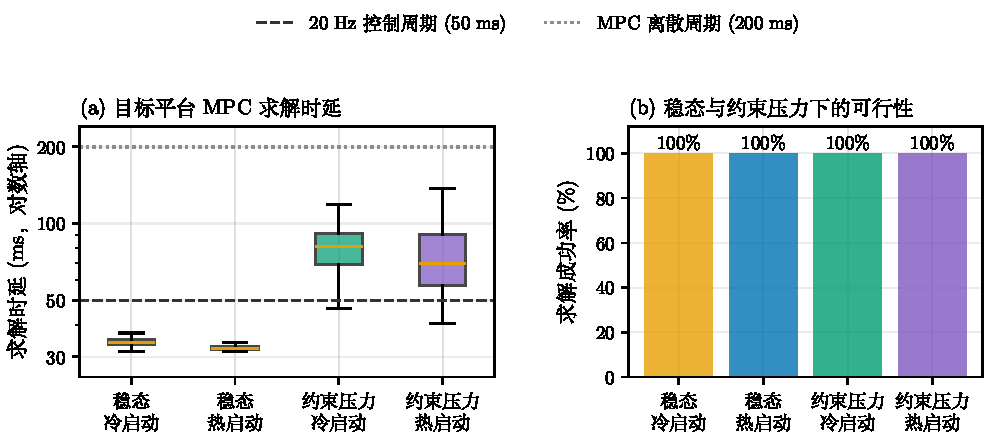
\includegraphics[width=0.96\linewidth,height=0.40\textheight,keepaspectratio,alt={Jetson Orin NX 稳态与约束压力档 MPC wall time 分布及求解成功率}]{../real_experiments/jetson_realtime/figures/jetson_mpc_latency_and_success.pdf}
\caption{Jetson Orin NX 上 MPC 稳态与约束压力档的求解 wall time 分布及成功率（25 W、8 核；求解器微基准）}\label{fig:ch05-jetson-mpc-realtime}
\end{figure}
\FloatBarrier

同一短时 clean run 共记录 60 个整机资源样本，覆盖 30.224 s；CPU mean/p95/max 为 39.9\%/60.0\%/75.1\%，内存 mean/max 为 4838.2/4918.6 MiB，最高温度为 57.4\textdegree C，0.5 s 采样间隔的 p95 为 0.505 s。CPU 分阶段均值为 idle/steady/stress=34.3\%/42.6\%/38.3\%。这些 CPU/GPU、内存和温度是 Jetson 整机遥测，不是求解器进程独占归因；空闲段本身仍含桌面负载。第~\ref{sec:ch05-5-3-1}节 已完成当前容器--真实 PC104 拓扑的 30 min 通信与控制软件栈稳态，但未记录 Jetson \texttt{tegrastats} 温度、频率和功耗，故不能替代目标机 thermal soak。

通信侧 4504 个有效上行到达间隔的 p50/p95/p99 为 58.005/85.721/86.095 ms。帧号审计中的 1501 次零增量是重复状态帧，而非 1501 帧丢失；大于 1 的前向跨帧为 0、估算丢帧为 0。first-echo RTT 与求解 wall time 来自不同执行路径，仍不得相加为 ADC--EKF--行为树--控制--PC104 的完整端到端时延。当前结果关闭的是目标平台求解器短时可运行性、真实 PC104 正常通信与固件回显、PC104 故障到行为树的同步零执行器触发链，以及当前拓扑 30 min 稳态；尚未关闭真实 ADC/DVL 输入下的完整调度、Jetson thermal soak 或 Jetson--PC104 单向物理时延。这些边界集中收束于第~\ref{sec:ch05-5-6}节，后续刻度见第~\ref{sec:ch06-6-3}节。

\subsection{故障注入自救逻辑验证}\label{sec:ch05-5-3-4}

故障注入自救逻辑采用等价规则完成统计对照：1000 次持续漏水用于响应延迟，100 条阈值噪声序列用于颤振，500 次低电压、漏水和近底穿越组合故障用于遗漏与死锁判定。两种决策架构均保持 100 ms 紧急响应和 100\% 组合故障生存率，证据只用于决策核心逻辑，不外推为通信链路或执行机构的系统级响应。

\section{综合结果与方法适用性讨论}\label{sec:ch05-5-5-9}

本章仿真和数字孪生结果仅支撑相应模型、场景与评价口径下的算法结论，不能直接外推为真实 AUV 的性能。水动力参数、相关噪声、通信时延分布及 Jetson 的散热和资源竞争均可能改变闭环表现；真实系统还需以实测时延、热稳定性、传感器噪声和执行器响应复验。各项已完成处置、不可外推范围及剩余验证见第~\ref{sec:ch05-5-6}节和附录表~\ref{tab:ch05-negative-results}。

在现场首验的任务选择上，本文将\emph{已知目标、经审查的短直线段和预对准走廊}对应的单次浅角穿越作为有限横向巡检候选；连续多横切保留为解决宽先验的主动测线扩展。保存的种子 101 轨迹中，前者约走 333 m／1122 s，后者的三／四段配方约走 576／731 m、耗时 1824／2272 s，均只巡检约 80 m；输入流向、先验和走廊不同，数值用于任务资源说明而非同条件性能排名。更关键的是，多横切目前只有合成横流和目标身份消息，且解析覆盖余量很紧，不能把仿真配方直接冻结为实艇路线。首验需以目标与邻缆的真实线位、导航采集来源、走廊和 PC104 收帧／滑行原始包替换这些夹具；未通过时系统仍可保留磁异常观测和有状态拒绝，埋深不发布。这样把方法贡献固定在主动空间观测与分层许可，同时使近期物理验收目标有明确、可核查的适用条件。

分层许可还应传递到最终自治执行出口。独立进程短探针发现，算法最后一条正向目标速度至夹具收到首条零目标速度、零 PID 输出分别相隔约 $1.013$、$1.188~\mathrm{s}$；其间夹具仍收到三条正 PID，接收次序受 DDS 和回调排队影响，不能断言控制器收到零目标后仍计算正推力。专用巡检桥因此增加上游目标速度的 $0.5~\mathrm{s}$ 墙钟时效门：安装版桥的独立本地 UDP 回环中，新鲜目标与 PID 对应 $25\%$ 主推；目标过期或显式 Hold、PID 仍新鲜时，桥输出零主推，命令保活亦如此。该门减少旧算法决策被新控制命令掩盖的授权风险，但安装版短 ROS--PID--桥--PVS 同次尝试仍在 DDS 等待阶段超时，未证明健康段持续输出；桥门也不能缩短算法本身的回调延迟或证明板端执行、艇体停车。磁场形失配时埋深拒绝与此执行时效门属于不同的许可层，现场仍须分别验收。

为定位持续性约束，另用独立进程以 $10~\mathrm{Hz}$ 供给导航、磁场与协方差，并分别记录实际发送与观察端接收时刻。原候选因长决策回调造成导航失鲜后永久锁存；默认关闭的后续候选改在决策起点保存输入快照，将短时输入缺口置于有边界和时限的零速 Hold，并由独立进程核对导航、磁测及目标指令的原始来源时间戳。仅核对接收时间的一趟曾在故障守卫窗漏放一条正向目标指令；增加来源时间戳后，两趟有限合成守卫窗分别记录 $23/23$、$16/16$ 条零速指令。最后一趟无计时追踪运行的故障守卫窗为目标速度 $15/15$、PID $6/6$ 零输出，恢复段 $28/34$ 条目标速度转正，说明软件能够在部分短暂缺口后重新授权。然而该趟健康供数最大空档 $0.349~\mathrm{s}$、最终目标指令最大空档 $0.512~\mathrm{s}$，均未达到预设 $0.25/0.30~\mathrm{s}$ 连续性门；全部十四趟独立探针均未通过严格总门。此处只支持失鲜分层处置与来源拒绝的有限回归，不构成 $10~\mathrm{Hz}$ 持续巡检或实艇现场放行证据；候选保持默认关闭。

进一步将算法决策周期改为 $0.2/0.4~\mathrm{s}$，或使监督门在排队后只取最新候选与传感器样本，另外五趟独立探针仍全部未过原严格门：四趟输入最大发送间隔小于 $0.25~\mathrm{s}$，但五趟最终目标速度都有零速，最佳一趟仅 $34/40$ 条正向、最大输出空档 $0.415~\mathrm{s}$。原健康窗从首次任务发布起算，含正常建链等待；用原始事件剥离任务发布后的首 $1~\mathrm{s}$ 作诊断，五趟稳态仍均出现零速，因此负结论并非只由启动等待造成。此处不把后验稳态窗口偷换成新的通过门限；最新值队列开关已从产品配置撤回。

因此，后续现场冻结不以本机短探针的均值或单次恢复替代目标平台完整任务验收。追加的 $0.2~\mathrm{m/s}$ 低速合成探针仍未过严格总门；其中健康供数合格的一趟仅有 $24/42$ 条正向最终目标指令，独立接收端还发现 $63$ 条正向消息中 $9$ 条到达时已超过本次 $1.3~\mathrm{s}$ 候选年龄上限。这提示仅检查门内来源年龄会遗漏晚到旧消息，但本机仿真时钟与 DDS 排队不能给出实艇发生率。本文据此将同次时序包的可执行审计合同升级为接收端来源时效检查：逐周期保存监督门收到的导航、磁测、协方差与候选来源年龄，独立观察最终目标速度及其原始来源时间、PID、UDP 下行与 PC104 实收，并在实测对时误差内分别检查健康段最大空档、正向消息到达年龄和故障后持续零命令。构造数据验证了检查器能拒绝门内有效但到达已旧的目标指令、旧导航来源戳、零速漏放和板端命令不符；真实包尚未采集，故这只建立可复核的验收方法，不增加现场许可或持续巡检通过率。

作为接收端补项，巡检专用 PID 又增加默认关闭的正向目标指令来源时效门。隔离 DDS 墙钟试验中，来源年龄 $1.030~\mathrm{s}$ 的旧指令触发零推，随后年龄 $0.030~\mathrm{s}$ 的新指令产生 $13.53\%$ 推力，说明本地控制律可在拒绝旧来源后恢复；全包测试 98 项通过。该试验没有算法、桥、板端或完整任务参与，因此仅证明 PID 层条件门生效，不改变上述连续性和现场放行结论。

图~\ref{fig:ch05-inspection-same-session-receipt}进一步把同次固定供数、候选、监督门决定、独立 DDS 接收和 PID 输出投到同一单调时间轴。合成健康窗中，$23/35$ 条最终目标速度为正，独立接收时又有 $4/23$ 条正向消息的来源年龄超过声明的 $1.3~\mathrm{s}$；输入最大缺口 $0.263~\mathrm{s}$ 也略超预设门。图的作用是使“候选生成、许可决定和消息实际到达”可分别审计，而不是宣称本机短任务满足连续运行。另两趟同配置诊断重复观察到接收时已旧的正向消息；一趟故障守卫窗还收到晚到正向目标速度，因此执行端自身的来源时效门与目标平台同次整包验收仍不可省略。

\begin{figure}[htbp]
\centering
\includegraphics[width=0.96\linewidth,height=0.52\textheight,keepaspectratio,alt={同次合成固定供数、算法候选、监督门决定、独立 DDS 接收和 PID 输出事件，以及正向最终 Setpoint 在接收时超过候选来源年龄限值的观测}]{experiments/fwhm_v2/64_same_session_ros_receipt_timeline.pdf}
\caption{巡检候选的同次监督门与独立 DDS 接收来源时效诊断。图中是本机合成短探针；橙色菱形表示正向消息到达时来源年龄已超过本次声明限值，不代表实艇失效率。}
\label{fig:ch05-inspection-same-session-receipt}
\end{figure}

图~\ref{fig:ch05-inspection-finite-current-clock} 的八条保存合成航迹经独立重算，七条完成有限路线，一条反向流阶跃未到端但在撤权后连续 $241$ 周期保持 Setpoint、PID 和本地协议零推进；后者在零推力期间仍有 $5.683~\mathrm{m}$ 的 PVS 位移。该任务结果与运行时序是两种不同判据：另起独立 DDS 接收进程的分进程 PVS 短试，磁测最大接收空档为 $1.280/1.334~\mathrm{s}$；移除在线 PVS、开环重放历史动态航迹的两趟短试仍为 $1.167/0.820~\mathrm{s}$，最终目标速度分别仅 $0/46$、$1/34$ 条为正，均未运行到 Confirm 或 Track。动态重放重新合成磁测与声呐且不把控制指令反馈给载体，不能与完整航迹拼成一次实时闭环；声呐名义频率不同的两趟也不是受控降频对照。这些答问诊断不改变图~\ref{fig:ch05-inspection-finite-current-clock} 的受限方法结论，却进一步说明目标平台完整任务的同次输入--输出--板端时序验收尚未完成。

\paragraph{限定条件下的磁巡检仿真复核}
为固定可独立引用的磁算法结果，本文进一步用当前源码、既有 PID、72 字节协议编解码和原生 PVS，在已知孤立直线磁源、理想导航、零横流和 $6~\mathrm{m}$ 先验横偏条件下复跑单直导线与偶极包络各三个磁噪声种子，以及三个无源对照。采用既有 F 配方的 $20~\mathrm{m}$ 前向接入；名义 $80~\mathrm{m}$ 任务两端各留 $5~\mathrm{m}$ 缓冲，核验核心为 $[5,75]~\mathrm{m}$。六条正例均完成任务并完整穿过核心段，三条无源例均拒绝进入跟踪。核心段内全部 Track 样本计入评价，包括回归修正，其真实横偏平均绝对误差为 $0.771$--$0.774~\mathrm{m}$、最大为 $1.321~\mathrm{m}$，满足预设平均不超过 $1~\mathrm{m}$、最大不超过 $2~\mathrm{m}$ 的门；埋深均保持空值，九条运行均无异常退出或非有限状态。初始零接入配方的完整核心平均误差约 $1.064~\mathrm{m}$，未通过同一门限；仅筛选巡检业务标签会漏掉回归阶段，因此不采用该筛样统计。本次未修改磁算法或控制律。图~\ref{fig:ch05-current-magnetic-simulation-closure} 把过程、中心估计与完整沿程误差放在同一视图中；这项独立复验说明有限横向巡检可以在声明的仿真条件下成立，且不依赖未经标定的深度发布。固定二维磁包络、理想导航和仿真步长不构成高度/姿态耦合、ROS 调度或实物时序验收，亦不将六条正例外推为任意海况成功率。

\begin{figure}[htbp]
\centering
\includegraphics[width=0.96\linewidth,height=0.52\textheight,keepaspectratio,alt={当前磁巡检源码在限定条件下的搜索、主动横切、前向接入和有限跟踪；两场形中心估计与六条航迹的真实横向误差，含核心段全部回归修正}]{experiments/fwhm_v2/71_current_magnetic_simulation_closure.pdf}
\caption{当前磁巡检算法的限定条件仿真复核。阴影为 $70~\mathrm{m}$ 核验段，两端缓冲不计为核心覆盖；全部核心 Track 样本计入误差，埋深保持独立空值。地图横纵轴比例不同。}
\label{fig:ch05-current-magnetic-simulation-closure}
\end{figure}

\subsection{证据边界与负结果归因}\label{sec:ch05-5-6}

本节是全章证据边界的索引。磁探测计量、ES-EKF 统计一致性、在线先验几何前提、不确定性感知控制、CBF 与原生因子闭环、实物通信与端到端时延的已完成证据、可写结论与剩余验证，统一列于附录表~\ref{tab:ch05-negative-results}。结果小节仅保留与其结论直接相关的限定。

\section{本章小结}\label{sec:ch05-5-8}

本章把实验结果收束为三条仿真主线和一个面向实物的证据容器。状态估计主线说明，ES-EKF 在多扰动、多随机种子条件下能够保持连续输出，并通过分源 NIS、长时程相位敏感性、实测背景回放和 Huber 更新把统计一致性与观测失配边界拆开说明；控制与安全主线说明，地形跟随、复杂路径预瞄、UA-MPC、CBF、安全仲裁和原生因子闭环共同构成可审计的近底巡检控制证据，但不同控制层级的优势区必须分别解释，不能把某一单项指标扩展为全场景最优；端到端海缆巡检数字孪生主线说明，系统在干净先验、先验畸变和满足磁观测前提的闭环恢复条件下完成了行业标准风格的验收判定，并把横偏、埋深、不确定度、置信度、运行状态和验收标志组织成同一运行话题链；ADC--TMR 噪声回放主线进一步证明，真实采集链背景可以以可追溯的 ROS2 量测输入进入闭环，而不改变本文对安全边界的审慎结论。

三条仿真主线之外，低成本磁采集、SK2301 窄带等效分辨率、45 Hz 复 I/Q 联合反演、磁外参标定链路、PC104 时序探针和同步双脑安全实验为实物部署提供了物理锚点。它们当前支撑的是``关键链路可实现、接口可复用、真实执行脑故障可同步驱动 ROS2 仲裁与任务降级、零执行器软件栈可稳定运行 30 min''，而不是完整水下自主巡检已经闭合。全章因此形成的结论边界是清晰的：算法链路已在可重复仿真与半实物口径下闭合，真实 PC104 通信、watchdog 与跨层状态链已完成验收；实物层还需沿磁采集链、等效海缆扫描、磁卫生、Jetson 热稳定、声呐接入、执行机构静态/动态响应和水域试验逐级补强。统计、场景、接口和计量边界已集中于第~\ref{sec:ch05-5-6}节 与附录表~\ref{tab:ch05-negative-results}，不在本章小结重复展开。
